% Please do not edit this file, expanded-paper.tex!
% It was generated automatically from its master file paper.tex, by programs/expand.js
% Get everything from https://github.com/haroldthimbleby/improving-science
% 
% This file expands the LaTeX file (paper.tex), which has complex dependencies,
%   to make this simple LaTeX file (expanded-paper.tex)
%     that depends on nothing, apart from its standard document class.
%       This expanded file depends on no other files, as instead
%         each required file's text was input and expanded recursively - search for '% expand' in the expanded file below.
% 
% (The original file is dependent on BibTeX (.bst and .bbl files), a macro file, table of contents,
%   its own and other files' .aux files,
%     as well as various data files in the directory generated
%       etc. All these file dependencies have been removed.)
% 

\makeatletter
\relax 
\providecommand\hyper@newdestlabel[2]{}
\providecommand\HyperFirstAtBeginDocument{\AtBeginDocument}
\HyperFirstAtBeginDocument{\ifx\hyper@anchor\@undefined
\global\let\oldnewlabel\newlabel
\gdef\newlabel#1#2{\newlabelxx{#1}#2}
\gdef\newlabelxx#1#2#3#4#5#6{\oldnewlabel{#1}{{#2}{#3}}}
\AtEndDocument{\ifx\hyper@anchor\@undefined
\let\newlabel\oldnewlabel
\fi}
\fi}
\global\let\hyper@last\relax 
\gdef\HyperFirstAtBeginDocument#1{#1}
\providecommand\HyField@AuxAddToFields[1]{}
\providecommand\HyField@AuxAddToCoFields[2]{}
\citation{a=b}
\citation{write-for-life}
\citation{abelson}
\citation{nature-chatgpt}
\newlabel{FirstPage}{{}{1}{}{Doc-Start}{}}
\@writefile{toc}{\contentsline {section}{\numberline {1}Introduction}{1}{section.1}\protected@file@percent }
\citation{sommerville,knight}
\citation{computational-thinking-wing,computational-thinking}
\citation{ICmodel,avianFluModel,originalICmodel}
\citation{ICmodel,avianFluModel,originalICmodel}
\citation{reproducibility-crisis,rescience}
\@writefile{toc}{\contentsline {section}{\numberline {2}Background}{2}{section.2}\protected@file@percent }
\@writefile{lot}{\contentsline {table}{\numberline {1}{\ignorespaces Overview of peer-reviewed paper sample, broken down further in Table \ref {table-summary}. Survey methodology and data is provided in the Supplemental Material. (The survey does not include the motivating papers \cite  {ICmodel,avianFluModel,originalICmodel}, none of which provide code or code summaries; see section \ref {section-pandemic-modeling}.)}}{3}{table.1}\protected@file@percent }
\newlabel{table-overview}{{1}{3}{Overview of peer-reviewed paper sample, broken down further in Table \ref {table-summary}. Survey methodology and data is provided in the \supplement . (The survey does not include the motivating papers \cite {ICmodel,avianFluModel,originalICmodel}, none of which provide code or code summaries; see section \ref {section-pandemic-modeling}.)}{table.1}{}}
\@writefile{lot}{\contentsline {table}{\numberline {2}{\ignorespaces Breakdown of pilot survey of peer-reviewed science papers relying on code. }}{3}{table.2}\protected@file@percent }
\newlabel{table-summary}{{2}{3}{Breakdown of pilot survey of peer-reviewed science papers relying on code}{table.2}{}}
\@writefile{lot}{\contentsline {table}{\numberline {3}{\ignorespaces The TOP committee's recommended levels for journal article code transparency. Level 0 is provided for a comparison that does not meet any TOP requirements. Concerns about the interpretation of ``reproduced independently,'' as required at level 4, are raised in section \ref {reproducibility-concerns}.}}{3}{table.3}\protected@file@percent }
\newlabel{TOPtable}{{3}{3}{The TOP committee's recommended levels for journal article code transparency. Level 0 is provided for a comparison that does not meet any TOP requirements. Concerns about the interpretation of ``reproduced independently,'' as required at level 4, are raised in section \ref {reproducibility-concerns}}{table.3}{}}
\citation{temperature}
\citation{form}
\citation{acm-algorithms}
\citation{hoare-correctness}
\citation{jupyter-study}
\citation{trisovic}
\citation{jupyter-study}
\citation{trisovic}
\citation{trisovic}
\@writefile{toc}{\contentsline {subsection}{\numberline {2.a}Code quality concerns}{4}{subsection.2.1}\protected@file@percent }
\newlabel{related-work}{{2.a}{4}{Code quality concerns}{subsection.2.1}{}}
\citation{machine-learning-reproducibility,no-raw-data,data-access,reproducible-manifesto,reproducibility-crisis}
\citation{joss}
\citation{rescience}
\citation{TOP}
\citation{TOP-wiki}
\citation{jupyter-study}
\citation{MMR-fraud}
\citation{misconduct-issues}
\citation{machine-learning-reproducibility}
\citation{elns}
\@writefile{toc}{\contentsline {subsection}{\numberline {2.b}Computable papers}{5}{subsection.2.2}\protected@file@percent }
\newlabel{computable-papers}{{2.b}{5}{Computable papers}{subsection.2.2}{}}
\citation{ICmodel}
\citation{perkel-review}
\citation{maneage}
\citation{maneage}
\citation{LP,LP-book}
\citation{relit}
\citation{notebook-patent}
\citation{jupyter-history}
\citation{knitr}
\citation{spec-led-design}
\citation{RAPstandard}
\@writefile{toc}{\contentsline {subsection}{\numberline {2.c}RAP: Reproducible Analytical Pipelines}{7}{subsection.2.3}\protected@file@percent }
\newlabel{RAP-section}{{2.c}{7}{RAP: Reproducible Analytical Pipelines}{subsection.2.3}{}}
\citation{rap,goldacre,turing-way}
\@writefile{lot}{\contentsline {table}{\numberline {4}{\ignorespaces A simplified schematic of the publication pipeline. For clarity, the pipeline has been linearized; in general, there will be repetitive cyclic iteration and refinement. The RAP and RAP{\tt  +}\ approaches encode the normally manual steps in the pipeline workflow so that they can be run automatically, and hence reproduce the results that underpin the final paper. The encoded RAP{\tt  +}\ algorithms can be shared with other scientists, scrutinized, simplified and optimized, and themselves turned into publishable objects --- they are scientific instruments, just like thermometers or DNA sequencers. Additional schematics are provided in section \ref {supplement-RAP-diagrams} in the Supplemental Material.}}{8}{table.4}\protected@file@percent }
\newlabel{fig-pipeline}{{4}{8}{A simplified schematic of the publication pipeline. For clarity, the pipeline has been linearized; in general, there will be repetitive cyclic iteration and refinement. The RAP and \RAPstar \ approaches encode the normally manual steps in the pipeline workflow so that they can be run automatically, and hence reproduce the results that underpin the final paper. The encoded \RAPstar \ algorithms can be shared with other scientists, scrutinized, simplified and optimized, and themselves turned into publishable objects --- they are scientific instruments, just like thermometers or DNA sequencers. Additional schematics are provided in section \ref {supplement-RAP-diagrams} in the \supplement }{table.4}{}}
\@writefile{lot}{\contentsline {table}{\numberline {5}{\ignorespaces A minimum standard of RAP, based on the UK Statistics Authority summary \cite  {RAPstandard}.}}{8}{table.5}\protected@file@percent }
\newlabel{figure-RAP-summary}{{5}{8}{A minimum standard of RAP, based on the UK Statistics Authority summary \cite {RAPstandard}}{table.5}{}}
\citation{MMR-fraud}
\citation{a=b}
\citation{Courtes}
\@writefile{toc}{\contentsline {subsubsection}{\numberline {2.c.1}Potential code}{9}{subsubsection.2.3.1}\protected@file@percent }
\@writefile{toc}{\contentsline {subsubsection}{\numberline {2.c.2}RAP as research}{9}{subsubsection.2.3.2}\protected@file@percent }
\citation{Courtes}
\citation{Courtes}
\citation{apa-statistics,Mariusz-reporting,science-statistics-recommendations}
\citation{example-stats}
\citation{science-statistics-recommendations}
\citation{Spiegelhalter}
\citation{paul-hci,pnas-stats}
\citation{paul-hci,pnas-stats}
\citation{Ben,se-bias}
\@writefile{toc}{\contentsline {section}{\numberline {3}The statistics/code analogy}{10}{section.3}\protected@file@percent }
\newlabel{statistics-computation-analogy}{{3}{10}{The statistics/code analogy}{section.3}{}}
\citation{sas9.2}
\citation{whitty}
\newlabel{section-vicious-cycles}{{3}{11}{The statistics/code analogy}{section.3}{}}
\@writefile{toc}{\contentsline {subsection}{\numberline {3.a}The siren call of over-fitting code}{11}{subsection.3.1}\protected@file@percent }
\newlabel{over-fit}{{3.a}{11}{The siren call of over-fitting code}{subsection.3.1}{}}
\citation{over-fit}
\citation{over-fit}
\citation{may-simple}
\citation{dyson}
\newlabel{name-example-footnote}{{5}{12}{}{Hfootnote.5}{}}
\citation{assurance-case}
\@writefile{lof}{\contentsline {figure}{\numberline {1}{\ignorespaces Much computational science is concerned with finding plausible multi-dimensional models that fit models to data with the aim of extrapolating or predicting new results from them. Shown here is notional sample of experimental 2D data (the dots), a linear least squares regression, and an exact polynomial model. The over-fitted polynomial model fits the sample \emph  {exactly\/}, but since the experimental data is presumably subject to random error (indicated by the confidence interval, itself estimated) the linear model would generally be considered a better description of the experimental data.}}{13}{figure.1}\protected@file@percent }
\newlabel{fig-overfit}{{1}{13}{Much computational science is concerned with finding plausible multi-dimensional models that fit models to data with the aim of extrapolating or predicting new results from them. Shown here is notional sample of experimental 2D data (the dots), a linear least squares regression, and an exact polynomial model. The over-fitted polynomial model fits the sample \emph {exactly\/}, but since the experimental data is presumably subject to random error (indicated by the confidence interval, itself estimated) the linear model would generally be considered a better description of the experimental data}{figure.1}{}}
\@writefile{toc}{\contentsline {section}{\numberline {4}The conventional role of code}{13}{section.4}\protected@file@percent }
\citation{assessing-quality}
\citation{fixit}
\citation{Hammurabi}
\@writefile{toc}{\contentsline {subsection}{\numberline {4.a}The deceptive simplicity of code}{14}{subsection.4.1}\protected@file@percent }
\newlabel{deceptive-simplicity-of-code}{{4.a}{14}{The deceptive simplicity of code}{subsection.4.1}{}}
\citation{cite-code,TOP}
\citation{prisma}
\citation{engima}
\citation{critiques,diagnosis-reviews}
\@writefile{toc}{\contentsline {subsection}{\numberline {4.b}The low status of coding}{15}{subsection.4.2}\protected@file@percent }
\newlabel{lowCodeStatus}{{4.b}{15}{The low status of coding}{subsection.4.2}{}}
\@writefile{toc}{\contentsline {subsection}{\numberline {4.c}The critical role of code is often ignored}{15}{subsection.4.3}\protected@file@percent }
\newlabel{central-role-of-code}{{4.c}{15}{The critical role of code is often ignored}{subsection.4.3}{}}
\newlabel{PRISMA-statement}{{4.c}{15}{The critical role of code is often ignored}{subsection.4.3}{}}
\@writefile{toc}{\contentsline {subsection}{\numberline {4.d}Bugs, code and programming}{15}{subsection.4.4}\protected@file@percent }
\newlabel{knowledge}{{4.d}{15}{Bugs, code and programming}{subsection.4.4}{}}
\citation{knuth}
\citation{essence-of-software,fixit}
\citation{popper-conjectures-refutations}
\citation{preventable-book}
\@writefile{toc}{\contentsline {subsection}{\numberline {4.e}Long-term problems of unreliable code}{16}{subsection.4.5}\protected@file@percent }
\citation{preventable-book}
\citation{science-review}
\citation{diagnosis-reviews}
\citation{tripod}
\citation{diagnosis-reviews}
\citation{diagnosis-reviews}
\citation{nature-summary,ICmodel}
\citation{avianFluModel,originalICmodel}
\citation{ICmodel,avianFluModel,originalICmodel}
\citation{tweet}
\citation{ferguson-interview}
\citation{basic-reproducibilty}
\citation{ferguson-resign}
\@writefile{toc}{\contentsline {section}{\numberline {5}State of the art}{17}{section.5}\protected@file@percent }
\@writefile{toc}{\contentsline {subsection}{\numberline {5.a}Case study: Pandemic modeling}{17}{subsection.5.1}\protected@file@percent }
\newlabel{section-pandemic-modeling}{{5.a}{17}{Case study: Pandemic modeling}{subsection.5.1}{}}
\citation{tweet}
\citation{forsyth,Normal-Distributions}
\citation{misra}
\citation{spark}
\citation{haskell}
\citation{thumbs-up}
\citation{nature-summary,ICmodel}
\citation{codecheck,thumbs-up}
\citation{codecheck}
\citation{ICmodel}
\citation{codecheck-certificate}
\citation{codecheck}
\citation{codecheck-certificate}
\newlabel{discuss-covid-sim}{{5.a}{18}{Case study: Pandemic modeling}{subsection.5.1}{}}
\@writefile{toc}{\contentsline {subsection}{\numberline {5.b}Concerns with reproducibility}{18}{subsection.5.2}\protected@file@percent }
\newlabel{reproducibility-concerns}{{5.b}{18}{Concerns with reproducibility}{subsection.5.2}{}}
\citation{codecheck,thumbs-up}
\citation{codecheck-certificate}
\citation{NVP}
\citation{nvp-ferguson}
\citation{essence-of-software}
\citation{notebooks,popper-conjectures-refutations,tripod,prisma,nih-policy,nih-nature}
\citation{refactoring}
\citation{bad-code}
\citation{bad-code}
\citation{pseudo}
\citation{chinese}
\citation{relit}
\citation{flu-model}
\citation{nature-review}
\citation{nature-review}
\citation{psychological-modeling}
\citation{psychological-modeling}
\citation{actr}
\citation{psychological-modeling}
\citation{Ben,nature-review,se-bias}
\citation{ourReview}
\citation{hamming}
\citation{NVP}
\@writefile{toc}{\contentsline {subsection}{\numberline {5.c}Beyond pandemic modeling}{20}{subsection.5.3}\protected@file@percent }
\newlabel{section-science-beyond-pandemic-modeling}{{5.c}{20}{Beyond pandemic modeling}{subsection.5.3}{}}
\citation{unfinished}
\citation{unfinished,lancet-unfinished}
\citation{hoare}
\citation{machine-learning-reproducibility}
\citation{relit}
\citation{preclinical-reproducibility}
\citation{fair,fair-principles}
\citation{nih-policy}
\citation{nih-nature}
\newlabel{section-discussion}{{5.c}{21}{Beyond pandemic modeling}{subsection.5.3}{}}
\@writefile{toc}{\contentsline {subsection}{\numberline {5.d}The lop-sided emphasis on data}{21}{subsection.5.4}\protected@file@percent }
\newlabel{critique-fair}{{5.d}{21}{The lop-sided emphasis on data}{subsection.5.4}{}}
\citation{notebooks}
\citation{cbc}
\citation{ethics-code}
\@writefile{toc}{\contentsline {section}{\numberline {6}Rethinking science that uses code}{22}{section.6}\protected@file@percent }
\newlabel{summary}{{6}{22}{Rethinking science that uses code}{section.6}{}}
\@writefile{toc}{\contentsline {subsection}{\numberline {6.a}Software Engineering Boards}{22}{subsection.6.1}\protected@file@percent }
\citation{acm-artifacts}
\citation{redmill,iec61508}
\citation{hoare-unreasonable}
\citation{basic-reproducibilty,open-source}
\citation{ABCs-SE}
\citation{mrb}
\citation{mrb}
\citation{relit,Executable-Paper}
\citation{computational-thinking-wing,computational-thinking}
\@writefile{toc}{\contentsline {subsection}{\numberline {6.b}Extending RAP to RAP{\tt  +}}{23}{subsection.6.2}\protected@file@percent }
\newlabel{RAPstar-section}{{6.b}{23}{Extending RAP to \RAPstar }{subsection.6.2}{}}
\citation{RMarkdown}
\citation{lepton}
\@writefile{toc}{\contentsline {subsection}{\numberline {6.c}The paper as a scientific laboratory}{24}{subsection.6.3}\protected@file@percent }
\newlabel{paper-as-lab}{{6.c}{24}{The paper as a scientific laboratory}{subsection.6.3}{}}
\citation{landauer,thimbleby-landauer}
\@writefile{toc}{\contentsline {subsection}{\numberline {6.d}Action must be interdisciplinary}{25}{subsection.6.4}\protected@file@percent }
\@writefile{toc}{\contentsline {subsection}{\numberline {6.e}Methodological statements}{25}{subsection.6.5}\protected@file@percent }
\citation{no-raw-data}
\citation{data-access}
\citation{assurance-case}
\citation{debt}
\newlabel{mentionPLOSandIEEE}{{6.e}{26}{Methodological statements}{subsection.6.5}{}}
\@writefile{toc}{\contentsline {subsection}{\numberline {6.f}Training to reduce technical debt}{26}{subsection.6.6}\protected@file@percent }
\newlabel{technical-debt}{{6.f}{26}{Training to reduce technical debt}{subsection.6.6}{}}
\citation{fixit}
\citation{jpm}
\citation{jpm}
\@writefile{toc}{\contentsline {subsection}{\numberline {6.g}Benefits beyond science}{27}{subsection.6.7}\protected@file@percent }
\newlabel{benefits-beyond-science}{{6.g}{27}{Benefits beyond science}{subsection.6.7}{}}
\citation{jpm-report}
\citation{jpm}
\citation{hoare-unreasonable}
\citation{excel-fiasco}
\citation{science-delays}
\@writefile{toc}{\contentsline {subsection}{\numberline {6.h}Approaches to further work}{28}{subsection.6.8}\protected@file@percent }
\@writefile{toc}{\contentsline {section}{\numberline {7}Conclusions}{28}{section.7}\protected@file@percent }
\citation{tweet,ferguson-interview}
\citation{whitty}
\citation{fixit}
\citation{reproducibility,relit,popper-conjectures-refutations}
\citation{parliamentary-evidence,my-parliamentary-evidence}
\bibstyle{revisedCompJ}
\bibdata{paper.bib}
\bibcite{a=b}{1}
\bibcite{write-for-life}{2}
\bibcite{abelson}{3}
\bibcite{nature-chatgpt}{4}
\bibcite{sommerville}{5}
\bibcite{knight}{6}
\bibcite{computational-thinking-wing}{7}
\bibcite{computational-thinking}{8}
\bibcite{ICmodel}{9}
\bibcite{avianFluModel}{10}
\bibcite{originalICmodel}{11}
\bibcite{reproducibility-crisis}{12}
\bibcite{rescience}{13}
\bibcite{temperature}{14}
\bibcite{form}{15}
\bibcite{acm-algorithms}{16}
\bibcite{hoare-correctness}{17}
\bibcite{jupyter-study}{18}
\bibcite{trisovic}{19}
\bibcite{machine-learning-reproducibility}{20}
\bibcite{no-raw-data}{21}
\bibcite{data-access}{22}
\bibcite{reproducible-manifesto}{23}
\bibcite{joss}{24}
\bibcite{TOP}{25}
\bibcite{TOP-wiki}{26}
\bibcite{MMR-fraud}{27}
\bibcite{misconduct-issues}{28}
\bibcite{elns}{29}
\bibcite{perkel-review}{30}
\bibcite{maneage}{31}
\bibcite{LP}{32}
\bibcite{LP-book}{33}
\bibcite{relit}{34}
\bibcite{notebook-patent}{35}
\bibcite{jupyter-history}{36}
\bibcite{knitr}{37}
\bibcite{spec-led-design}{38}
\bibcite{RAPstandard}{39}
\bibcite{rap}{40}
\bibcite{goldacre}{41}
\bibcite{turing-way}{42}
\bibcite{Courtes}{43}
\bibcite{apa-statistics}{44}
\bibcite{Mariusz-reporting}{45}
\bibcite{science-statistics-recommendations}{46}
\bibcite{example-stats}{47}
\bibcite{Spiegelhalter}{48}
\bibcite{paul-hci}{49}
\bibcite{pnas-stats}{50}
\bibcite{Ben}{51}
\bibcite{se-bias}{52}
\bibcite{sas9.2}{53}
\bibcite{whitty}{54}
\bibcite{over-fit}{55}
\bibcite{may-simple}{56}
\bibcite{dyson}{57}
\bibcite{assurance-case}{58}
\bibcite{assessing-quality}{59}
\citation{assessing-quality-conference}
\bibcite{fixit}{60}
\bibcite{Hammurabi}{61}
\bibcite{cite-code}{62}
\bibcite{prisma}{63}
\bibcite{engima}{64}
\bibcite{critiques}{65}
\bibcite{diagnosis-reviews}{66}
\bibcite{knuth}{67}
\bibcite{essence-of-software}{68}
\bibcite{popper-conjectures-refutations}{69}
\bibcite{preventable-book}{70}
\bibcite{science-review}{71}
\bibcite{tripod}{72}
\bibcite{nature-summary}{73}
\bibcite{tweet}{74}
\bibcite{ferguson-interview}{75}
\bibcite{basic-reproducibilty}{76}
\bibcite{ferguson-resign}{77}
\bibcite{forsyth}{78}
\bibcite{Normal-Distributions}{79}
\bibcite{misra}{80}
\bibcite{spark}{81}
\bibcite{haskell}{82}
\bibcite{thumbs-up}{83}
\bibcite{codecheck}{84}
\bibcite{codecheck-certificate}{85}
\bibcite{NVP}{86}
\bibcite{nvp-ferguson}{87}
\bibcite{notebooks}{88}
\bibcite{nih-policy}{89}
\bibcite{nih-nature}{90}
\bibcite{refactoring}{91}
\bibcite{bad-code}{92}
\bibcite{pseudo}{93}
\bibcite{chinese}{94}
\bibcite{flu-model}{95}
\bibcite{nature-review}{96}
\bibcite{psychological-modeling}{97}
\bibcite{actr}{98}
\bibcite{ourReview}{99}
\bibcite{hamming}{100}
\bibcite{unfinished}{101}
\bibcite{lancet-unfinished}{102}
\bibcite{hoare}{103}
\bibcite{preclinical-reproducibility}{104}
\bibcite{fair}{105}
\bibcite{fair-principles}{106}
\bibcite{cbc}{107}
\bibcite{ethics-code}{108}
\bibcite{acm-artifacts}{109}
\bibcite{redmill}{110}
\bibcite{iec61508}{111}
\bibcite{hoare-unreasonable}{112}
\bibcite{open-source}{113}
\bibcite{ABCs-SE}{114}
\bibcite{mrb}{115}
\bibcite{Executable-Paper}{116}
\bibcite{RMarkdown}{117}
\bibcite{lepton}{118}
\bibcite{landauer}{119}
\bibcite{thimbleby-landauer}{120}
\bibcite{debt}{121}
\bibcite{jpm}{122}
\bibcite{jpm-report}{123}
\bibcite{excel-fiasco}{124}
\bibcite{science-delays}{125}
\bibcite{reproducibility}{126}
\bibcite{parliamentary-evidence}{127}
\bibcite{my-parliamentary-evidence}{128}
\citation{parliamentary-evidence}
\bibcite{assessing-quality-conference}{129}
\def\continueSectionNumbers{7}
\def\continueTableNumbers{5}
\def\continueFigureNumbers{1}
\def\continueFootnoteNumbers{13}
\def\continuePageNumbers{35}
\newlabel{LastPage}{{}{35}}
\gdef \@abspage@last{35}

\makeatother
\documentclass{comjnl}
\usepackage{ragged2e}
\usepackage{amsmath}
\usepackage{amssymb}

\setcounter{tocdepth}{3}

%----
  \setlength\textheight{220mm}
%----

% expand macros.tex
% due to finding out that PDF doesn't work everywhere, here's where we define the image type we're using for imaged created by the Mathematica notebooks
\def\imageFileSuffix{jpg}


\usepackage[hyphens]{url}
\usepackage{hyperref}
\usepackage{xcolor}
\usepackage{longtable}
\usepackage{cite}

\renewcommand\thesubsection{\thesection.\alph{subsection}}
\renewcommand\thesubsubsection{\thesection.\alph{subsection}.\arabic{subsubsection}}

\def\httpURL#1{\href{http://#1}{\textcolor{blue}{#1}}}
\def\LONGhttpURL#1#2{\href{http://#1}{\textcolor{blue}{#2}}}

\makeatletter
    \def\do@url@hyp{\do/}
    \usepackage{moreverb}
\makeatother

\DeclareUrlCommand\doi{\def\UrlLeft{{\textrm{DOI}\ } }}
\DeclareUrlCommand\url{\def\UrlLeft{{\textrm{URL}\ } }}
\DeclareUrlCommand\midurl{\def\UrlLeft{}\allowbreak }
	
\renewcommand{\thefootnote}{\arabic{footnote}}

\def\mytitle{Improving science that uses code}
\def\supplement{Supplemental Material}

\def\citeeg#1{[e.g., \citenum{#1}]}

% calculate rounded percentages
\newcount \t
\newcount \tu
\def\pc#1#2{\t = #1%
\multiply \t by 100000%
\divide \t by #2% ?? 0 times percentage
\tu = \t
\divide \t by 1000% percentage, but no idea of remainder
\multiply \t by 1000% 1000 times percentage, with 00 as bottom digits
\advance \tu by -\t% bottom two digits
\divide \t by 1000\relax%
% round to nearest integer
% if ending in > .5 round up
% if ending in exactly .5 round towards nearest even number
\ifnum \tu > 500 % round up
	\advance \t by 1 
\else
	\ifnum \tu = 500 
		\ifodd \t % it's odd, so round up to even number 
			\advance \t by 1
		\else % leave rounded to even number 	
		\fi
	\fi
\fi
\the\t\%}

% code to make digits into blocks of 3 (as in 1000 -> 1 000)
\def\xBlockSep{\textcolor{red}{\hskip 0.3em :}\hskip 0.3em} % International Standards are to use a small space. UK typically uses a comma
% NOTE currently, the few decimal numbers (eg 0.000 5) use hskip explicitly, since defining \xBlockSep as a comma would definitely be wrong for decimals
\newcount\xdigitBlockn
\newcount\xdigitBlocktmp
\def\xdigitBlock#1{%
        \xdigitBlockn=#1\relax
        \ifnum \xdigitBlockn < 0
                $-$%
                \xdigitBlockn = -\xdigitBlockn
        \fi
        \let \xdigitBlockpptemp \empty
        \loop \ifnum \xdigitBlockn > 999
                \xdigitBlocktmp = \xdigitBlockn
                \divide \xdigitBlockn by 1000
                \xdigitBlocktmp = \numexpr \xdigitBlocktmp - 1000*\xdigitBlockn \relax
                \edef \xdigitBlockpptemp{\xBlockSep\ifnum \xdigitBlocktmp < 100  0\ifnum \xdigitBlocktmp < 10 0\fi\fi \the\xdigitBlocktmp \xdigitBlockpptemp}%
        \repeat
        \the\xdigitBlockn
        \xdigitBlockpptemp
}

\def\digitBlock#1{\hbox{\xdigitBlock{#1}}}

% simple macro to use a number register to pluralize (add an s) to words....
% \plural{\t}{fred} => \the\t\ freds if plural, or => one fred if singular
\def\plural#1#2{\ifnum #1=1 
	one #2%
\else
	\the#1\ #2s%
\fi}

% initialiseBibliography <title> <starting number> <introductory text>
\newcount \bibciten \bibciten=0
\def\initialiseBibliography#1#2#3{% title, starting citation number, an initial paragraph
	\global\def\refname{\arabic{section} #1}
    \global\def\unnumberedrefname{#1}
    \global\bibciten=#2
    \global\def\startBibliography{#3}
}

\def\bibskip{\vskip 1ex} % the gap between bib items generated by data.js

% read in any constants defined from the JSON or Git data
% expand generated/constants.tex
% Generated by programs/data.js
\def\journalBreakdown{\emph{Lancet Digital Health\/} ($N=6$), \emph{Nature Digital Medicine\/} ($N=12$) and \emph{Royal Society Open Science\/} ($N=14$)}
\def\tabularJournalBreakdown{&\hbox to 3em {\hfill 6}\hskip 1em \emph{Lancet Digital Health}\\&\hbox to 3em {\hfill 12}\hskip 1em \emph{Nature Digital Medicine}\\&\hbox to 3em {\hfill 14}\hskip 1em \emph{Royal Society Open Science}\\}
\global\newcount \dataN \global\dataN=32
\global\newcount \countAuthors \global\countAuthors=264
\global\newcount \countHasBreach \global\countHasBreach=11
\global\newcount \countHasPolicy \global\countHasPolicy=26
\global\newcount \countUsesVersionControlRepository \global\countUsesVersionControlRepository=10
\global\newcount \counthasDataRepository \global\counthasDataRepository=9
\global\newcount \countNoCodeInRepo \global\countNoCodeInRepo=1
\global\newcount \numberOfJournals \global\numberOfJournals=3
\global\newcount \countCodetested \global\countCodetested=0
\global\newcount \hasDevelopedRigorously \global\hasDevelopedRigorously=0
\global\newcount \countFields \global\countFields=36
\global\newcount \countCommentedOut \global\countCommentedOut=7
\global\newcount \countNotCommentedOut \global\countNotCommentedOut=2
\global\newcount \countMissingCode \global\countMissingCode=1
\global\def \averagePagesPerAuthor{1.2916666666666667}
% end expanding generated/constants.tex
% expand generated/metadata.tex
% shell script (make-metadata.sh) generated LaTeX variable values counting errors detected by data.js
\newcount \JSONerrorCount
\JSONerrorCount = 30
\newcount \dataVariableCount
\dataVariableCount = 62
% end expanding generated/metadata.tex
% expand generated/covidsimSummary.tex
% data calculated from the Ferguson covid-sim repo
\def \covidsimkLOC {25}
\def \covidsimfiles {229}
\def \covidsimdata{734 Mb}
% end expanding generated/covidsimSummary.tex
% expand generated/clone-date.tex
% date generated by running generated/allGitRepos.sh downloading Git repos
\def\clonedate {\ignorespaces 7 June 2023}
\def\cloneyear {2023}
\def\clonemonth {06}
% end expanding generated/clone-date.tex

\newcount \pubdelayinmonths
\pubdelayinmonths=\cloneyear
\advance \pubdelayinmonths by -2019 % submitted in 2019
\multiply \pubdelayinmonths by 12
\advance \pubdelayinmonths by -6 % submitted in June
\advance \pubdelayinmonths by \clonemonth

\def\monthname#1{\ifcase#1 \or 
January\or 
February\or 
March\or 
April\or 
May\or 
June\or 
July\or 
August\or 
September\or 
October\or 
November\or 
December\fi}

\def\numbertoname#1{\ifcase #1 zero\or one\or two\or three\or four\or five\or six\or seven\or eight\or nine\else #1\fi}
\def\Numbertoname#1{\ifcase #1 Zero\or One\or Two\or Three\or Four\or Five\or Six\or Seven\or Eight\or Nine\else #1\fi}

\def\clonewhen{\monthname{\clonemonth} \cloneyear}

\def\RAPstar{RAP{\tt +}}
\def\RAPstars{RAPs{\tt +}}
\def\RAPstarp#1{RAP{\tt +}#1}
\def\italicRAPstar{RAP{\tt +}}
% end expanding macros.tex
% expand generated/page-lengths.tex
% Generated by programs/data.js
\expandafter\def\csname pagelength-MetricSelectionFramework\endcsname{17}
\expandafter\def\csname pagelength-PENet\endcsname{9}
\expandafter\def\csname pagelength-PostoperativeOutcomes.RiskNet\endcsname{10}
\expandafter\def\csname pagelength-philter-ucsf\endcsname{8}
\expandafter\def\csname pagelength-AI-CDSS-Cardiovascular-Silo\endcsname{6}
\expandafter\def\csname pagelength-SiameseChange\endcsname{9}
\expandafter\def\csname pagelength-lactModel\endcsname{13}
\expandafter\def\csname pagelength-LRM\endcsname{22}
\expandafter\def\csname pagelength-manifold-ga\endcsname{7}
\expandafter\def\csname pagelength-blast-ct\endcsname{8}
\newcount \gitPages \gitPages=109
\newcount \totalPages \totalPages=341
% end expanding generated/page-lengths.tex

\makeatletter
      % expand appendix.aux 
\relax 
\providecommand\hyper@newdestlabel[2]{}
\providecommand\HyperFirstAtBeginDocument{\AtBeginDocument}
\HyperFirstAtBeginDocument{\ifx\hyper@anchor\@undefined
\global\let\oldnewlabel\newlabel
\gdef\newlabel#1#2{\newlabelxx{#1}#2}
\gdef\newlabelxx#1#2#3#4#5#6{\oldnewlabel{#1}{{#2}{#3}}}
\AtEndDocument{\ifx\hyper@anchor\@undefined
\let\newlabel\oldnewlabel
\fi}
\fi}
\global\let\hyper@last\relax 
\gdef\HyperFirstAtBeginDocument#1{#1}
\providecommand\HyField@AuxAddToFields[1]{}
\providecommand\HyField@AuxAddToCoFields[2]{}
\citation{vancouver}
\citation{hamming}
\citation{fixit}
\citation{cosmos}
\@writefile{toc}{\contentsline {section}{\numberline {8}Further issues for Software Engineering Boards (SEBs)}{38}{section.8}\protected@file@percent }
\@writefile{toc}{\contentsline {subsection}{\numberline {8.a}Relationships of SEBs to Ethics Boards}{38}{subsection.8.1}\protected@file@percent }
\citation{ethics-paper}
\citation{ai-ethics}
\citation{science-lancet1,science-lancet2,lancet-learning}
\citation{jvs1,jvs2,jvs3}
\citation{sommerville,knight}
\citation{cosmos}
\citation{swebok}
\citation{turing-way}
\citation{wpf}
\citation{humphrey}
\citation{managers}
\@writefile{toc}{\contentsline {subsection}{\numberline {8.b}SEBs are necessary but not sufficient}{39}{subsection.8.2}\protected@file@percent }
\@writefile{toc}{\contentsline {section}{\numberline {9}Software engineering best practice}{39}{section.9}\protected@file@percent }
\newlabel{supplement-best-practice}{{9}{39}{Software engineering best practice}{section.9}{}}
\@writefile{toc}{\contentsline {subsection}{\numberline {9.a}Requirements}{39}{subsection.9.1}\protected@file@percent }
\citation{differential-equations}
\citation{cbc}
\citation{spark}
\citation{misra}
\citation{hoare}
\citation{hoare}
\citation{numerals}
\citation{heedless}
\@writefile{toc}{\contentsline {subsection}{\numberline {9.b}Formal methods}{40}{subsection.9.2}\protected@file@percent }
\@writefile{toc}{\contentsline {subsection}{\numberline {9.c}Defensive programming}{40}{subsection.9.3}\protected@file@percent }
\citation{onlyPaperWithChecks}
\citation{tweet,plos}
\citation{heedless}
\citation{spark}
\citation{haskell}
\citation{basic-reproducibilty,reproducibility}
\citation{NVP}
\citation{avianFluModel}
\citation{ICmodel}
\citation{flu-model}
\citation{excel1,excel2}
\citation{npm}
\@writefile{toc}{\contentsline {subsection}{\numberline {9.d}Using inappropriate programming languages undermines reliability}{41}{subsection.9.4}\protected@file@percent }
\@writefile{toc}{\contentsline {subsection}{\numberline {9.e}Open source and version control}{41}{subsection.9.5}\protected@file@percent }
\citation{open-source}
\citation{sommerville,knight,NVP}
\citation{assurance-case}
\citation{LP}
\citation{relit}
\citation{hci1,hci2}
\@writefile{toc}{\contentsline {subsection}{\numberline {9.f}Rigorous testing}{42}{subsection.9.6}\protected@file@percent }
\@writefile{toc}{\contentsline {subsection}{\numberline {9.g}Good documentation and record keeping}{42}{subsection.9.7}\protected@file@percent }
\citation{flexibility}
\citation{iso}
\citation{178C}
\citation{fixit}
\@writefile{toc}{\contentsline {subsection}{\numberline {9.h}Usability}{43}{subsection.9.8}\protected@file@percent }
\newlabel{supplement-material-makefiles}{{9.h}{43}{Usability}{subsection.9.8}{}}
\@writefile{toc}{\contentsline {subsection}{\numberline {9.i}Reusing quality solutions}{43}{subsection.9.9}\protected@file@percent }
\@writefile{toc}{\contentsline {subsection}{\numberline {9.j}Simplicity}{43}{subsection.9.10}\protected@file@percent }
\@writefile{toc}{\contentsline {subsection}{\numberline {9.k}Compliance with standards}{43}{subsection.9.11}\protected@file@percent }
\citation{peerReview,knight}
\citation{ssi-report,ssi-url}
\citation{acm-artifacts}
\citation{security-engineering,cyber-cacm}
\citation{example-numerical-error}
\citation{hamming}
\citation{Schneier}
\citation{electronic-evidence}
\@writefile{toc}{\contentsline {subsection}{\numberline {9.l}Effective multidisciplinary teamwork}{44}{subsection.9.12}\protected@file@percent }
\@writefile{toc}{\contentsline {subsection}{\numberline {9.m}Continuous Professional Development (CPD)}{44}{subsection.9.13}\protected@file@percent }
\@writefile{toc}{\contentsline {subsection}{\numberline {9.n}Security and other factors}{44}{subsection.9.14}\protected@file@percent }
\@writefile{toc}{\contentsline {subsection}{\numberline {9.o}Software is a human activity}{44}{subsection.9.15}\protected@file@percent }
\citation{fixit}
\citation{popper-conjectures-refutations}
\citation{simon-artificial}
\citation{dunning-kruger,dunning-kruger-numeracy}
\citation{dunning-kruger}
\citation{fixit}
\citation{enigma}
\citation{harking}
\citation{viruses}
\@writefile{toc}{\contentsline {section}{\numberline {10}Code, data, and publication}{45}{section.10}\protected@file@percent }
\newlabel{supplement-on-code-data-publication}{{10}{45}{Code, data, and publication}{section.10}{}}
\citation{viruses}
\citation{strachey}
\@writefile{toc}{\contentsline {subsection}{\numberline {10.a}When magic numbers become magic code}{46}{subsection.10.1}\protected@file@percent }
\citation{henderson}
\citation{paper-usesRMarkdown}
\citation{RMarkdown}
\@writefile{toc}{\contentsline {subsection}{\numberline {10.b}When data is code}{47}{subsection.10.2}\protected@file@percent }
\@writefile{toc}{\contentsline {subsection}{\numberline {10.c}Exploiting code as data for more reliable science}{47}{subsection.10.3}\protected@file@percent }
\@writefile{toc}{\contentsline {subsection}{\numberline {10.d}When data is text: Exploiting code for reliable publication}{47}{subsection.10.4}\protected@file@percent }
\citation{Spiegelhalter}
\@writefile{toc}{\contentsline {subsection}{\numberline {10.e}Data and polynomials used in the paper}{48}{subsection.10.5}\protected@file@percent }
\@writefile{toc}{\contentsline {subsection}{\numberline {10.f}Comparing conventional and RAP approaches}{48}{subsection.10.6}\protected@file@percent }
\newlabel{supplement-RAP-diagrams}{{10.f}{48}{Comparing conventional and RAP approaches}{subsection.10.6}{}}
\@writefile{toc}{\contentsline {section}{\numberline {11}The Spiegelhalter trustworthiness questions}{48}{section.11}\protected@file@percent }
\newlabel{supplement-Spiegelhalter-section}{{11}{48}{The Spiegelhalter trustworthiness questions}{section.11}{}}
\@writefile{lof}{\contentsline {figure}{\numberline {2}{\ignorespaces The common basic --- error-prone and obsolete --- approach to scientific authoring is to use code to help generate analyses and diagrams, then manually copy and paste the selected results into the publication. Note that the publication, including the results, can be edited arbitrarily, and typically the results published will have been edited and modified (if only for typographical purposes) from those actually generated by the code.}}{49}{figure.2}\protected@file@percent }
\newlabel{supplement-fig:basic}{{2}{49}{The common basic --- error-prone and obsolete --- approach to scientific authoring is to use code to help generate analyses and diagrams, then manually copy and paste the selected results into the publication. Note that the publication, including the results, can be edited arbitrarily, and typically the results published will have been edited and modified (if only for typographical purposes) from those actually generated by the code}{figure.2}{}}
\@writefile{lof}{\contentsline {figure}{\numberline {3}{\ignorespaces When the code is in a spreadsheet, such as Microsoft Excel, the code is generally hidden from sight. The data copied \& pasted into a publication may or may not be calculated from data in other cells (such as column totals). Records are rarely taken of these manual processes, and, anyway, typically it is impossible to be certain exactly what has been copied unless very great care is taken. In consequence, if a spreadsheet is modified, it is haphazard what results are updated and corrected in the publication. }}{49}{figure.3}\protected@file@percent }
\newlabel{supplement-fig:excel}{{3}{49}{When the code is in a spreadsheet, such as Microsoft Excel, the code is generally hidden from sight. The data copied \& pasted into a publication may or may not be calculated from data in other cells (such as column totals). Records are rarely taken of these manual processes, and, anyway, typically it is impossible to be certain exactly what has been copied unless very great care is taken. In consequence, if a spreadsheet is modified, it is haphazard what results are updated and corrected in the publication}{figure.3}{}}
\@writefile{lof}{\contentsline {figure}{\numberline {4}{\ignorespaces Improving over the normal approach (figure \ref {supplement-fig:basic}), data and diagrams are placed in the publication using a programmed, systematic approach. In the present paper, this was done by generating text files of \LaTeX  \ definitions (represented by boxes in the central column of the schematic), hence providing \LaTeX  \ names for all of the code-generated values. Since the copying of results into a publication is automated and easy, any improvements to the results (such as correcting errors) are made by improving the code --- which therefore contributes to improving all future-generated results too. Not shown, but in well-engineered code, documentation will also be generated, such as by using tools such as JavaDoc or Doxygen.}}{50}{figure.4}\protected@file@percent }
\newlabel{supplement-fig:rap}{{4}{50}{Improving over the normal approach (figure \ref {supplement-fig:basic}), data and diagrams are placed in the publication using a programmed, systematic approach. In the present paper, this was done by generating text files of \LaTeX \ definitions (represented by boxes in the central column of the schematic), hence providing \LaTeX \ names for all of the code-generated values. Since the copying of results into a publication is automated and easy, any improvements to the results (such as correcting errors) are made by improving the code --- which therefore contributes to improving all future-generated results too. Not shown, but in well-engineered code, documentation will also be generated, such as by using tools such as JavaDoc or Doxygen}{figure.4}{}}
\@writefile{toc}{\contentsline {subsection}{\numberline {11.a}How trustworthy are the numbers?}{50}{subsection.11.1}\protected@file@percent }
\@writefile{lof}{\contentsline {figure}{\numberline {5}{\ignorespaces In a notebook system, such as \emph  {Mathematica\/} or Jupyter, a single document --- the notebook --- integrates the publication, the code, any notes, as well as all the results. The code generates results and images that are automatically (and reliably) inserted in place into the notebook, usually right after the code that generates them. Some parts of the notebook are marked or selected to be printed as the publication, thus allowing most if not all code to be hidden from the final publication. In well-engineered code, the notebook will directly contain full documentation. Note that in most systems, notebooks can import and generate arbitrary data (images, sounds, sensor data, etc).}}{51}{figure.5}\protected@file@percent }
\newlabel{supplement-fig:notebook}{{5}{51}{In a notebook system, such as \emph {Mathematica\/} or Jupyter, a single document --- the notebook --- integrates the publication, the code, any notes, as well as all the results. The code generates results and images that are automatically (and reliably) inserted in place into the notebook, usually right after the code that generates them. Some parts of the notebook are marked or selected to be printed as the publication, thus allowing most if not all code to be hidden from the final publication. In well-engineered code, the notebook will directly contain full documentation. Note that in most systems, notebooks can import and generate arbitrary data (images, sounds, sensor data, etc)}{figure.5}{}}
\@writefile{toc}{\contentsline {subsection}{\numberline {11.b}How trustworthy is the source?}{51}{subsection.11.2}\protected@file@percent }
\citation{lancet-retracted}
\citation{science-lancet1,science-lancet2}
\citation{lancet-learning}
\@writefile{toc}{\contentsline {subsection}{\numberline {11.c}How trustworthy is the interpretation?}{52}{subsection.11.3}\protected@file@percent }
\@writefile{toc}{\contentsline {section}{\numberline {12}A pilot survey of computational science}{52}{section.12}\protected@file@percent }
\newlabel{supplement-survey-section}{{12}{52}{A pilot survey of computational science}{section.12}{}}
\@writefile{toc}{\contentsline {subsection}{\numberline {12.a}Selected journal case studies}{52}{subsection.12.1}\protected@file@percent }
\@writefile{toc}{\contentsline {subsubsection}{\numberline {12.a.1}\emph  {The Lancet\/}}{52}{subsubsection.12.1.1}\protected@file@percent }
\citation{jvs1}
\citation{jvs2,jvs3}
\citation{jvs1}
\citation{numerals}
\citation{fda}
\citation{ICmodel}
\citation{ICmodel}
\citation{ICmodel}
\@writefile{lot}{\contentsline {table}{\numberline {6}{\ignorespaces Conforming to the RAP{\tt  +}\ methodology, the abbreviated summary above was generated automatically, by using \texttt  {make data}. A full list of \texttt  {make} options is generated by \texttt  {make} or \texttt  {make help} when run on the Unix command line. }}{53}{table.6}\protected@file@percent }
\newlabel{supplement-table:options}{{6}{53}{Conforming to the \RAPstar \ methodology, the abbreviated summary above was generated automatically, by using \texttt {make data}. A full list of \texttt {make} options is generated by \texttt {make} or \texttt {make help} when run on the Unix command line}{table.6}{}}
\@writefile{toc}{\contentsline {subsubsection}{\numberline {12.a.2}\emph  {Journal of Vascular Surgery}}{53}{subsubsection.12.1.2}\protected@file@percent }
\newlabel{supplement-vascular-surgery-note}{{12.a.2}{53}{\emph {Journal of Vascular Surgery}}{subsubsection.12.1.2}{}}
\@writefile{toc}{\contentsline {subsection}{\numberline {12.b}Pilot paper sample}{53}{subsection.12.2}\protected@file@percent }
\@writefile{lot}{\contentsline {table}{\numberline {7}{\ignorespaces Overview of the peer-reviewed paper sample. (Convenient copy of main paper's table \ref {table-overview}.)}}{54}{table.7}\protected@file@percent }
\newlabel{supplement-table-overview}{{7}{54}{Overview of the peer-reviewed paper sample. (Convenient copy of main paper's table \ref {table-overview}.)}{table.7}{}}
\@writefile{lot}{\contentsline {table}{\numberline {8}{\ignorespaces Summary of survey results. (Convenient copy of main paper's table \ref {table-summary}.)}}{54}{table.8}\protected@file@percent }
\newlabel{supplement-table-summary}{{8}{54}{Summary of survey results. (Convenient copy of main paper's table \ref {table-summary}.)}{table.8}{}}
\citation{nature-review}
\@writefile{lot}{\contentsline {table}{\numberline {9}{\ignorespaces Sizes of repositories, with approximate sizes of code (in kLOC) and data for all available GitHub repositories reviewed in the survey, plus \texttt  {covid-sim} \cite  {ICmodel} for comparison. Sizes are approximate because in all repositories code and data are conceptually interchangeable (an issue explained in the Supplemental Material), so choices were made in the survey to avoid double-counting. Many repositories rely on downloading additional code and data, which is not counted in the table as the additional required material is not in the repository cited in the paper. At the time of cloning and checking all repositories in June 2023, paper [182]\ still had nothing in its repository except a single file still saying ``\ldots  \ code coming soon\nobreakspace  {}\ldots  ,'' despite 48\ months having already elapsed since the paper had claimed the code could be accessed in its repository.}}{55}{table.9}\protected@file@percent }
\newlabel{supplement-table-repo-summary}{{9}{55}{Sizes of repositories, with approximate sizes of code (in kLOC) and data for all available GitHub repositories reviewed in the survey, plus \texttt {covid-sim} \cite {ICmodel} for comparison. Sizes are approximate because in all repositories code and data are conceptually interchangeable (an issue explained in the \supplement ), so choices were made in the survey to avoid double-counting. Many repositories rely on downloading additional code and data, which is not counted in the table as the additional required material is not in the repository cited in the paper. At the time of cloning and checking all repositories in \clonewhen , paper \csname cite-PostoperativeOutcomes.RiskNet\endcsname \ still had nothing in its repository except a single file still saying ``\ldots \ code coming soon~\ldots ,'' despite \the \pubdelayinmonths \ months having already elapsed since the paper had claimed the code could be accessed in its repository}{table.9}{}}
\citation{open-source}
\citation{stability}
\@writefile{toc}{\contentsline {subsection}{\numberline {12.c}Summary of results}{56}{subsection.12.3}\protected@file@percent }
\newlabel{supplement-summary-of-results}{{12.c}{56}{Summary of results}{subsection.12.3}{}}
\citation{RS-policy}
\@writefile{toc}{\contentsline {subsubsection}{\numberline {12.c.1}Current code policies of sampled journals}{57}{subsubsection.12.3.1}\protected@file@percent }
\newlabel{supplement-journal-policies-section}{{12.c.1}{57}{Current code policies of sampled journals}{subsubsection.12.3.1}{}}
\citation{ref-1}
\citation{ref-2}
\citation{ref-3}
\citation{ref-4}
\citation{ref-5}
\citation{ref-6}
\citation{ref-7}
\citation{ref-8}
\citation{ref-9}
\citation{ref-10}
\citation{ref-11}
\citation{ref-12}
\citation{paper-usesRMarkdown}
\citation{ref-14}
\citation{onlyPaperWithChecks}
\citation{ref-16}
\citation{ref-17}
\citation{ethics-paper}
\citation{ref-19}
\citation{ref-20}
\citation{ref-21}
\citation{ref-22}
\citation{ref-23}
\citation{example-numerical-error}
\citation{ref-25}
\citation{ref-26}
\citation{ref-27}
\citation{ref-28}
\citation{ref-29}
\citation{ref-30}
\citation{ref-31}
\citation{ref-32}
\gdef \LT@i {\LT@entry 
    {2}{26.55563pt}\LT@entry 
    {1}{214.35622pt}\LT@entry 
    {1}{208.35622pt}}
\@writefile{toc}{\contentsline {subsubsection}{\numberline {12.c.2}Sample assessment and scoring}{58}{subsubsection.12.3.2}\protected@file@percent }
\citation{prisma}
\@writefile{toc}{\contentsline {subsection}{\numberline {12.d}Assessment criteria and methods}{60}{subsection.12.4}\protected@file@percent }
\newlabel{supplement-data-methods-subsection}{{12.d}{60}{Assessment criteria and methods}{subsection.12.4}{}}
\citation{fixit}
\citation{fixit}
\@writefile{toc}{\contentsline {subsubsection}{\numberline {12.d.1}Detecting and defending against error}{62}{subsubsection.12.4.1}\protected@file@percent }
\newlabel{supplement-detecting-against-error}{{12.d.1}{62}{Detecting and defending against error}{subsubsection.12.4.1}{}}
\citation{excel-fiasco}
\citation{latex-calculus}
\@writefile{toc}{\contentsline {subsubsection}{\numberline {12.d.2}Defending against system problems}{63}{subsubsection.12.4.2}\protected@file@percent }
\@writefile{toc}{\contentsline {subsubsection}{\numberline {12.d.3}Problems of restrictive journal policies}{63}{subsubsection.12.4.3}\protected@file@percent }
\newlabel{supplement-restrictive-policies}{{12.d.3}{63}{Problems of restrictive journal policies}{subsubsection.12.4.3}{}}
\bibstyle{revisedCompJ}
\bibdata{appendix.bib}
\bibcite{vancouver}{{{130}{}{{}}{{}}}}
\bibcite{cosmos}{{{131}{}{{}}{{}}}}
\bibcite{ai-ethics}{{{132}{}{{}}{{}}}}
\bibcite{science-lancet1}{{{133}{}{{}}{{}}}}
\bibcite{science-lancet2}{{{134}{}{{}}{{}}}}
\bibcite{lancet-learning}{{{135}{}{{}}{{}}}}
\bibcite{jvs1}{{{136}{}{{}}{{}}}}
\bibcite{jvs2}{{{137}{}{{}}{{}}}}
\bibcite{jvs3}{{{138}{}{{}}{{}}}}
\bibcite{swebok}{{{139}{}{{}}{{}}}}
\bibcite{wpf}{{{140}{}{{}}{{}}}}
\bibcite{humphrey}{{{141}{}{{}}{{}}}}
\bibcite{managers}{{{142}{}{{}}{{}}}}
\@writefile{toc}{\contentsline {section}{\numberline {13}Additional references for Supplemental Material}{64}{section.13}\protected@file@percent }
\bibcite{differential-equations}{{{143}{}{{}}{{}}}}
\bibcite{numerals}{{{144}{}{{}}{{}}}}
\bibcite{heedless}{{{145}{}{{}}{{}}}}
\bibcite{plos}{{{146}{}{{}}{{}}}}
\bibcite{excel1}{{{147}{}{{}}{{}}}}
\bibcite{excel2}{{{148}{}{{}}{{}}}}
\bibcite{npm}{{{149}{}{{}}{{}}}}
\bibcite{hci1}{{{150}{}{{}}{{}}}}
\bibcite{hci2}{{{151}{}{{}}{{}}}}
\bibcite{flexibility}{{{152}{}{{}}{{}}}}
\bibcite{iso}{{{153}{}{{}}{{}}}}
\bibcite{178C}{{{154}{}{{}}{{}}}}
\bibcite{peerReview}{{{155}{}{{}}{{}}}}
\bibcite{ssi-report}{{{156}{}{{}}{{}}}}
\bibcite{ssi-url}{{{157}{}{{}}{{}}}}
\bibcite{security-engineering}{{{158}{}{{}}{{}}}}
\bibcite{cyber-cacm}{{{159}{}{{}}{{}}}}
\bibcite{Schneier}{{{160}{}{{}}{{}}}}
\bibcite{electronic-evidence}{{{161}{}{{}}{{}}}}
\bibcite{simon-artificial}{{{162}{}{{}}{{}}}}
\bibcite{dunning-kruger}{{{163}{}{{}}{{}}}}
\bibcite{dunning-kruger-numeracy}{{{164}{}{{}}{{}}}}
\bibcite{enigma}{{{165}{}{{}}{{}}}}
\bibcite{harking}{{{166}{}{{}}{{}}}}
\bibcite{viruses}{{{167}{}{{}}{{}}}}
\bibcite{strachey}{{{168}{}{{}}{{}}}}
\bibcite{henderson}{{{169}{}{{}}{{}}}}
\bibcite{lancet-retracted}{{{170}{}{{}}{{}}}}
\bibcite{fda}{{{171}{}{{}}{{}}}}
\bibcite{stability}{{{172}{}{{}}{{}}}}
\bibcite{RS-policy}{{{173}{}{{}}{{}}}}
\bibcite{latex-calculus}{{{174}{}{{}}{{}}}}
\bibcite{ref-1}{{{175}{}{{}}{{}}}}
\bibcite{ref-2}{{{176}{}{{}}{{}}}}
\bibcite{ref-3}{{{177}{}{{}}{{}}}}
\bibcite{ref-4}{{{178}{}{{}}{{}}}}
\bibcite{ref-5}{{{179}{}{{}}{{}}}}
\@writefile{toc}{\contentsline {section}{\numberline {14}References for surveyed papers}{66}{section.14}\protected@file@percent }
\bibcite{ref-6}{{{180}{}{{}}{{}}}}
\bibcite{ref-7}{{{181}{}{{}}{{}}}}
\bibcite{ref-8}{{{182}{}{{}}{{}}}}
\bibcite{ref-9}{{{183}{}{{}}{{}}}}
\bibcite{ref-10}{{{184}{}{{}}{{}}}}
\bibcite{ref-11}{{{185}{}{{}}{{}}}}
\bibcite{ref-12}{{{186}{}{{}}{{}}}}
\bibcite{paper-usesRMarkdown}{{{187}{}{{}}{{}}}}
\bibcite{ref-14}{{{188}{}{{}}{{}}}}
\bibcite{onlyPaperWithChecks}{{{189}{}{{}}{{}}}}
\bibcite{ref-16}{{{190}{}{{}}{{}}}}
\bibcite{ref-17}{{{191}{}{{}}{{}}}}
\bibcite{ethics-paper}{{{192}{}{{}}{{}}}}
\bibcite{ref-19}{{{193}{}{{}}{{}}}}
\bibcite{ref-20}{{{194}{}{{}}{{}}}}
\bibcite{ref-21}{{{195}{}{{}}{{}}}}
\bibcite{ref-22}{{{196}{}{{}}{{}}}}
\bibcite{ref-23}{{{197}{}{{}}{{}}}}
\bibcite{example-numerical-error}{{{198}{}{{}}{{}}}}
\bibcite{ref-25}{{{199}{}{{}}{{}}}}
\bibcite{ref-26}{{{200}{}{{}}{{}}}}
\bibcite{ref-27}{{{201}{}{{}}{{}}}}
\bibcite{ref-28}{{{202}{}{{}}{{}}}}
\bibcite{ref-29}{{{203}{}{{}}{{}}}}
\bibcite{ref-30}{{{204}{}{{}}{{}}}}
\bibcite{ref-31}{{{205}{}{{}}{{}}}}
\bibcite{ref-32}{{{206}{}{{}}{{}}}}
\gdef \@abspage@last{34}
% end expanding appendix.aux 
\makeatother

\title{\mytitle} 
\author{Harold Thimbleby}
\shortauthors{Harold Thimbleby}
\affiliation{See Change Fellow in Digital Health, Swansea University}
\email{harold@thimbleby.net}

%\subject{Computational science (bioinformatics,~medical~computing,~etc)}

\keywords{Computational Science; Software Engineering; Reproducibility; Scientific scrutiny; Reproducible Analytic Pipeline (RAP \& \RAPstar\hskip -1pt)}

\received{30 April 2022}
\revised{8 June 2022, 3 January 2023, 31 January 2023, 12~May~2023 \& 7~June~2023} 
\volumenumber{00} \issuenumber{0} \volumeyear{2023}

%\orcid{0000-0003-2222-4243}

\begin{document}

\begin{abstract}
\justifying
\noindent
As code is now an inextricable part of science it should be supported by competent Software Engineering, analogously to statistical claims being properly supported by competent statistics. 

If and when code avoids adequate scrutiny, science becomes unreliable and unverifiable because results --- text, data, graphs, images, \emph{etc\/} --- depend on untrustworthy code.

Currently, scientists rarely assure the quality of the code they rely on, and rarely make it accessible for scrutiny. Even when available, scientists rarely provide adequate documentation to understand or use it reliably. 

\hskip 1em This paper proposes and justifies  ways to improve science using code:

\raggedright
\newdimen \mywidth \mywidth=\textwidth
\advance \mywidth by -3em

\def\indented#1{\vskip 1ex
\parshape 2 0em \textwidth 2em \mywidth 
\noindent 
\hbox to 2em{ #1.\hfill}\ignorespaces}

\indented 1
Professional Software Engineers can help, particularly in critical fields such as public health, climate change, and energy. 

\indented 2
``Software Engineering Boards,'' analogous to Ethics or Institutional Review Boards, should be instigated and used.

\indented 3
The Reproducible Analytic Pipeline (RAP) methodology can be generalized to cover code and Software Engineering methodologies, in a generalization this paper introduces called \RAPstarp. \RAPstar\ (or comparable interventions) could be supported and or even required in journal, conference, and funding body policies.

\vskip 1ex 
\justifying
\noindent
The paper's \supplement\ provides a summary of Software Engineering best practice relevant to scientific research, including further suggestions for \RAPstar\ workflows. 

\def\seprule{\vskip 2ex\hrule\vskip 2ex}
\seprule
\raggedright
\def\zq{\setbox0=\hbox{``}\hskip -0\wd0\copy0}
\zq Science is what we understand well enough to explain to a computer.''\\
\hfill {\rm Donald E. Knuth in $A=B$ \cite{a=b}}\\

\zq I have to write to discover what I am doing.''\\
\hfill {\rm Flannery O'Connor, quoted in \emph{Write for your life\/} \cite{write-for-life}}

\zq Criticism is the mother of methodology.''\\
\hfill {\rm Robert P. Abelson in \emph{Statistics as Principled Argument\/} \cite{abelson}}

\zq \hangindent \wd0 From its earliest times, science has operated by being open and transparent about methods and evidence, regardless of which technology has been in vogue.''\\
\hfill {\rm Editorial in \emph{Nature\/} \cite{nature-chatgpt}}

\seprule
\end{abstract}
\maketitle

%\section*{Author summary}
%
%%\includegraphics[width=1in,height=1.25in,clip,keepaspectratio]{HT}}]
%Harold Thimbleby PhD, FRCP (Edinburgh), Hon.\ FRSA, Hon.\ FRCP is See Change Fellow in Digital Health at Swansea University, Wales. His research focuses on human error and computer system design, particularly for healthcare. 
%%In addition to over 340 peer-reviewed and 188 invited publications, Harold has written several books, including \emph{Press On\/} (MIT Press, 2007), which was winner of the American Association of Publishers best book in computer science award.
%Harold won the British Computer Society Wilkes Medal. He is emeritus Gresham Professor of Geometry (a chair founded in 1597), and has been a Royal Society-Leverhulme Trust Senior Research Fellow and a Royal Society-Wolfson Research Merit Award holder. His latest book is  \emph{Fix IT: How to see and solve the problems of digital healthcare\/} \cite{fixit}.  See his web site, \texttt{www.harold.thimbleby.net}, for more details.

%\noindent\emph{This paper evidences widespread problems arising from scientific papers relying on inadequately defined computer and inaccessible code, which undermines peer-review and replication, and undermines scientific quality generally. The risks vary, depending on how critical a paper's claims may be: ranging from superficial for opinion papers, to serious for papers in domains such as medicine, public health, or policy. This paper contrasts the situation with the mature approach to using statistics, and goes on to make proposals to help address the problem. The proposals are feasible, and presented in the hope of motivating their (or better solutions) being implemented, tested, and refined.}

\section{Introduction}
Unreliable, often unstated and unexplored, code and computational dependencies (including using AI or ML) in science are widespread. Furthermore, code is rarely published or made accessible in a usable form; it is generally too onerous or impossible to verify or scrutinize. Ironically, computers should be able to make reproducibility easier, yet too often code and results claimed do not contribute to reliable science, and do not support verification, replication, or reproduction on which future science can be firmly based. 

\begin{table}
\vskip 1.2ex % align top of columns!
% expand table of contents paper.toc
\makeatletter
  \section*{\contentsname
    \@mkboth{\MakeUppercase\contentsname}{\MakeUppercase\contentsname}}
\makeatother\contentsline {section}{\numberline {1}Introduction}{1}{section.1}%
\contentsline {section}{\numberline {2}Background}{2}{section.2}%
\contentsline {subsection}{\numberline {2.a}Code quality concerns}{4}{subsection.2.1}%
\contentsline {subsection}{\numberline {2.b}Computable papers}{5}{subsection.2.2}%
\contentsline {subsection}{\numberline {2.c}RAP: Reproducible Analytical Pipelines}{7}{subsection.2.3}%
\contentsline {subsubsection}{\numberline {2.c.1}Potential code}{9}{subsubsection.2.3.1}%
\contentsline {subsubsection}{\numberline {2.c.2}RAP as research}{9}{subsubsection.2.3.2}%
\contentsline {section}{\numberline {3}The statistics/code analogy}{10}{section.3}%
\contentsline {subsection}{\numberline {3.a}The siren call of over-fitting code}{11}{subsection.3.1}%
\contentsline {section}{\numberline {4}The conventional role of code}{13}{section.4}%
\contentsline {subsection}{\numberline {4.a}The deceptive simplicity of code}{14}{subsection.4.1}%
\contentsline {subsection}{\numberline {4.b}The low status of coding}{15}{subsection.4.2}%
\contentsline {subsection}{\numberline {4.c}The critical role of code is often ignored}{15}{subsection.4.3}%
\contentsline {subsection}{\numberline {4.d}Bugs, code and programming}{15}{subsection.4.4}%
\contentsline {subsection}{\numberline {4.e}Long-term problems of unreliable code}{16}{subsection.4.5}%
\contentsline {section}{\numberline {5}State of the art}{17}{section.5}%
\contentsline {subsection}{\numberline {5.a}Case study: Pandemic modeling}{17}{subsection.5.1}%
\contentsline {subsection}{\numberline {5.b}Concerns with reproducibility}{18}{subsection.5.2}%
\contentsline {subsection}{\numberline {5.c}Beyond pandemic modeling}{20}{subsection.5.3}%
\contentsline {subsection}{\numberline {5.d}The lop-sided emphasis on data}{21}{subsection.5.4}%
\contentsline {section}{\numberline {6}Rethinking science that uses code}{22}{section.6}%
\contentsline {subsection}{\numberline {6.a}Software Engineering Boards}{22}{subsection.6.1}%
\contentsline {subsection}{\numberline {6.b}Extending RAP to RAP{\tt +}}{23}{subsection.6.2}%
\contentsline {subsection}{\numberline {6.c}The paper as a scientific laboratory}{24}{subsection.6.3}%
\contentsline {subsection}{\numberline {6.d}Action must be interdisciplinary}{25}{subsection.6.4}%
\contentsline {subsection}{\numberline {6.e}Methodological statements}{25}{subsection.6.5}%
\contentsline {subsection}{\numberline {6.f}Training to reduce technical debt}{26}{subsection.6.6}%
\contentsline {subsection}{\numberline {6.g}Benefits beyond science}{27}{subsection.6.7}%
\contentsline {subsection}{\numberline {6.h}Approaches to further work}{28}{subsection.6.8}%
\contentsline {section}{\numberline {7}Conclusions}{28}{section.7}%

% end expanding table of contents paper.toc

\vskip 3mm \hrule
\end{table}

This paper makes an explicit analogy between the use of statistics, which has clear standards for reliable use and presentation, and the use of code. Like statistics, code is often relied on to support key results in scientific publications, yet code is generally informal, inaccessible and incorrect. Just as sound experimental methods and sound statistics generally rely on professional specialist input, it is argued here that good use of code must rely on professional Software Engineering input \cite{sommerville,knight}, and more strategically on professional Computational Thinking \cite{computational-thinking-wing,computational-thinking} --- an accessible form of Software Engineering that consciously applies the ideas universally, far more widely than just to software and coding.

\begin{table*}
\begin{center}\sf\normalsize
\begin{tabular}{|rl|} \hline
\the\numberOfJournals&Journals\\
\the\dataN&Papers:\\
\tabularJournalBreakdown
\the\countAuthors&Published authors\\
\the\totalPages&Published journal pages\\
July 2020&Sample month\\ \hline
\end{tabular}
\end{center}\vskip -2ex
\caption{Overview of peer-reviewed paper sample, broken down further in Table \ref{table-summary}. Survey methodology and data is provided in the \supplement. (The survey does not include the motivating papers \cite{ICmodel,avianFluModel,originalICmodel}, none of which provide code or code summaries; see section \ref{section-pandemic-modeling}.)}
\label{table-overview}
\end{table*}

\begin{table*}
\begin{center}\sf\normalsize
% expand generated/summary-table.tex
% Generated by programs/data.js
\begin{tabular}{|rrrc|}\hline
Number of papers sampled relying on code&32&100\%&\\\hline\hline
\multicolumn{4}{|l|}{\textbf{Access to code}}\\
Some or all code available&12&38\%&\\
Some or all code in principle available on request&8&25\%&\\
Requested code actually made available (within 2 years 11 months${}^{\star}$)&0&0\%& \\\hline
 \multicolumn{4}{|l|}{{\textbf{Evidence of any software engineering practice}}}\\
Evidence program designed rigorously&{0}&{0\%}&\\
Evidence source code properly tested&{0}&{0\%}&\\
Evidence of any tool-based development&{0}&{0\%}&\\
Team or open source based development&{0}&{0\%}&\\
Other methods, e.g., independent coding methods&{1}&{3\%}&\\\hline
\multicolumn{4}{|l|}{\textbf{Documentation and comments}}\\
Substantial code documentation and comments&2&6\%&\\
Comments explain some code intent&3&9\%&\\
Procedural comments (e.g., author, date, copyright)&10&31\%&\\
No usable comments&17&53\%&\\\hline
\multicolumn{4}{|l|}{\textbf{Repository use}}\\
Used code repository (e.g., GitHub)&9&28\%&\\
Used data repository (e.g., Dryad or GitHub)&9&28\%&\\
Empty repository&1&3\%&\\\hline
\multicolumn{4}{|l|}{{\textbf{Evidence of documented processes}}}\\
Evidence of RAP/\RAPstar\ or any other principles in use to support scrutiny&{0}&{0\%}&\\\hline
\multicolumn{4}{|l|}{\textbf{Adherence to journal code policy (if any)}}\\
Papers published in journals with code policies&26&81\%&\\
Clear breaches of journal code policy (if any) & 11&42\%&(\emph{N}~=~26)\\
\hline\end{tabular}\\
\vskip 1ex ${}^{\star}$Time of 2 years 11 months is wait between code request and date of generating this table.% end expanding generated/summary-table.tex
\end{center}\vskip -2ex
\caption{Breakdown of pilot survey of peer-reviewed science papers relying on code. }
\label{table-summary}
\end{table*}

\begin{table*}
\newdimen\quarterwidth
\newdimen\separation
\separation=4.5mm
\quarterwidth=\textwidth
\advance\quarterwidth by -4\separation
\divide\quarterwidth by 4
\begin{center}
\noindent{\sf\begin{tabular}{|@{}c|c|c|c@{}|} \hline
\bfseries Level 0&
\bfseries Level 1&
\bfseries Level 2&
\bfseries Level 3 \\ \hline
\multicolumn{1}{|p{\quarterwidth}}{Journal encourages code sharing -- or says nothing.}&
\multicolumn{1}{|p{\quarterwidth}}{Article states whether code is available and, if so, where to access them.}&
\multicolumn{1}{|p{\quarterwidth}}{Code must be posted to a trusted repository. Exceptions must be identified at article submission.}&
\multicolumn{1}{|p{\quarterwidth}|}{Code must be posted to a trusted repository, and reported analyses will be reproduced independently before publication.} \\ \hline
\end{tabular}}\end{center}\vskip -2ex
\caption{The TOP committee's recommended levels for journal article code transparency. Level 0 is provided for a comparison that does not meet any TOP requirements. Concerns about the interpretation of ``reproduced independently,'' as required at level 4, are raised in section \ref{reproducibility-concerns}.}
\label{TOPtable}
\end{table*}

This paper was initially motivated by concerns about the poor quality of code used in high-profile epidemiology research because of its significance for informing and driving public health responses to the COVID-19 pandemic. A pilot survey implies that such problems are ubiquitous and by no means limited to epidemiology: see tables \ref{table-overview} \& \ref{table-summary} for a summary of the sample, and see the \supplement\ for further details of the survey. In the survey, \emph{no\/} papers claimed or provided evidence that their code was adequately tested or rigorously developed; \emph{none\/} used methodologies like RAP or \RAPstar\ (described below). Only one paper mentioned any Software Engineering methods, albeit simplistic and without technical details. 

In the survey sample 81\% of papers were published in leading journals that have code policies (which themselves are weak), but 42\% of surveyed papers published in those journals breached their own policies. One paper declared it had accessible code, but the relevant repository was and still remains empty. The findings are comparable to problems increasingly recognized for data and data access (reviewed in section \ref{related-work}): code problems form part of the \emph{reproducibility crisis\/} \citeeg{reproducibility-crisis,rescience} discussed throughout this paper.

This paper therefore argues that code should be developed and discussed in a professional, rigorous, and supportive environment that facilitates quality science with clear presentation and appropriately rigorous scrutiny of code. Its main contribution is to suggest straightforward ways to enable this. The proposals may not be ``the'' right or best ways, but it is hoped the case studies and arguments presented here persuade readers that the proposals are at least a productive way to start pointing in the right direction, and to inform raising the profile and constructively debating the issues more widely. 

An extensive online \supplement\ appendix to this paper provides additional resources, including brief details of many Software Engineering practices relevant to supporting quality science. The supplement will be of particular interest to research software engineers supporting non-software-specialist scientists.

\section{Background}
The discoveries and inventions of scientific technologies and instruments like microscopes, telescopes, and X-rays, drove and expanded the sciences. There are fascinating periods when new ideas and science unified; for example, thermometers could not measure temperature in any meaningful way until the underlying science was mature. For over a century, there was no agreement on definitions of temperature, how to calibrate thermometers, or what units they measured in. 

Paradoxically the science could not mature until there was consensus in scientific methodologies for thermometry, and having that consensus in turn depended on reproducible thermometer measurements; for example, scientists working in different places needed to know they were working with the ``same temperatures'' yet there was for a long period no consensus on what that meant. Contributing to reliable science depended on a thorough understanding of principles, including gradually fixing the confounding factors that were misunderstood \cite{temperature}.\footnote{One example: if the volume of mercury is chosen to measure temperature, a confounding factor is that the volume of the container measuring the volume of mercury also increases with temperature (but at a different rate), so the volume measurement is inaccurate.} 
Science matured from no quantitative interest in temperature, through a complex process of hand-in-hand theoretical-and-technical maturation, until today, when we have robust off-the-shelf instruments that measure temperature in reliable, repeatable, internationally standardized units, that follow international quality standards.

Computers are a unique, new technology, far more flexible and challenging than thermometers. Understanding computers and integrating them into science is far harder than the tortured development of modern thermometry. Computation not only expands science's paradigms and supports new discoveries (particularly with AI), but it also \emph{does\/} new science --- almost all modern laboratory instrumentation, including thermometers, is heavily computerized. Relying on computer models has become routine. The dependency of modern science on computers is far more tangled and complex than the now-resolved dependence on reliable temperature measurement; computers affect how scientists in all disciplines \emph{think}.

Pushing the boundaries of science, then, now involves pushing the boundaries of computer science. The synergy runs deep: for instance, while particle physics relies on powerful supercomputers, quantum physics itself is developing more powerful quantum computing.

``Computational science'' has come to mean a particular style of science based on developing and using explicit computational models, but, really, \emph{all\/} of science is now computational in this sense. 

Computational science is not just restricted to specialized fields like computational chemistry, genomics, big data~\ldots\ in all fields of science, computation is used at every step, from calculations of course, through note taking, sound and image processing, literature searches, analysis and statistics, correspondence with co-authors and editors, through to typesetting,  distributing and archiving the final publications. All areas of science are being profoundly computerized. Furthermore, developments in computer science themselves drive science such that earlier science is even becoming obsolete as the computer technology moves on \cite{form}.

\subsection{Code quality concerns}\label{related-work}
Publishing high quality computer code has been strongly advocated since the earliest times, such as the \emph{Communications of the ACM\/} in its first issue in its first volume published in 1958, where it outlined its algorithm publication policy. The new policy was illustrated with a square root algorithm \cite{acm-algorithms}. However, publishing code in the computer science literature is distinct from publishing high quality general science that depends on code, which is the particular concern of the present paper. Of course, as a special case, Computer Science too can also benefit from improving ways to reliably use code in general science.

In almost all published science, the code it relies on is taken for granted, just as in routine chemistry the quality of the glassware is not at issue. While chemists are trained in reliable methodologies, so taking quality glassware for granted is reasonable. Code is a newer innovation, and quality code is a current research programme in its own right, and has resulted in calls for a Grand Challenge research effort \cite{hoare-correctness}. Inevitably, because of these reasons taken collectively, much published science depends on unreliable code that is not explicitly discussed, was not peer-reviewed, and is not open to scrutiny, reproduction, or reuse by the scientific community. The situation with code is analogous to chemists using contaminated glassware with no awareness how its effects might be controlled or might affect results.

Is it a problem? A study of \digitBlock{863878} Python-coded Jupyter notebooks \cite{jupyter-study} found a 76\% failure rate for code to complete execution successfully. Trisovic \emph{et al.}\ \cite{trisovic} performed a  study of \digitBlock{9000} research codes written in the language R on Dataverse, an open-source repository maintained by Harvard University's Institute for Quantitative Social Sciences. They found a comparable result that 74\% of the code files analyzed failed. These results are consistent with this paper's findings, as summarized in tables \ref{table-overview} \& \ref{table-summary}. 

The authors of \cite{jupyter-study} make technical recommendations to improve reproducibility, such as ``Abstract code into functions, classes, and modules and test them.'' It will not be obvious for most practicing scientists how to do this, so, more generally, the authors of \cite{trisovic} recommend establishing Working Groups to support reproducible research --- and in fact Dataverse (the source of the \cite{trisovic} data) has already done so. These ideas may be compared to the present paper's proposal of Software Engineering Boards (SEBs), as discussed in detail in section \ref{summary}, supported by more specific suggestions in the \supplement.

These concerns about code are part of the reproducibility crisis for science generally \cite{machine-learning-reproducibility,no-raw-data,data-access,reproducible-manifesto,reproducibility-crisis}. Concern has led to new journals, \emph{Journal of Open Source Software\/} (JOSS) \cite{joss}, \emph{ReScience~C\/} \cite{rescience}, and  others, to explore and encourage the explicit replication of previously published research. 

To start to address code quality issues the Transparency and Openness Promotion Committee met in 2014, and has since been promoting Transparency and Openness Promotion, TOP, starting with journal publication policies \cite{TOP}. TOP covers citation standards, replication standards, and code standards amongst others. TOP recommends levels of compliance to their recommendations, where level 0 does not meet the standard, and levels 1 to 3 are increasingly stringent. The TOP levels for code are shown in table \ref{TOPtable}. The TOP standards continue to develop, and are now maintained on a wiki at \url{osf.io/9f6gx/wiki/Guidelines} \cite{TOP-wiki}. TOP can be compared with the Findable, Accessible, Interoperable and Reusable (FAIR) initiative, which places greater emphasis on data rather than code; FAIR itself is critiqued in section \ref{critique-fair}.

As the present paper argues, developing quality code is widely under-appreciated, which leads to a vicious cycle of lack of acknowledgement, invisibility, and being unable to recruit adequately competent coders (see section \ref{section-vicious-cycles}). The term \emph{research software engineer\/} was coined in 2012 to help address this problem, and to stimulate thinking about researchers' career paths. The Society of Research Software Engineering (\url{society-rse.org}) has been established to further promote research software engineer interests.  

There is no shortage of computational tools available to help address the problems. However, it should be noted that such tools are not a panacea, as the study \cite{jupyter-study} cited above makes clear. This suggests that human support for improving coding and reproduction quality, perhaps in the form of Working Groups or Boards, as this paper suggests, will be critical.

In addition to unintentional problems with code quality and reproducibility, actual scientific misconduct occurs when the outcome is intentional. While pure plagiarism, which is a form of misconduct, generally does not affect the quality of reported science, when data or code is fraudulently manipulated to have deceptive properties, the results are likely to be destructive. The notorious Wakefield MMR fraud claiming to link vaccines and autism published in \emph{The Lancet\/} took 12 years before it was retracted; this misconduct has been extraordinarily destructive \cite{MMR-fraud}. 

A recent meta-analysis of surveys of scientific misconduct estimates that nearly 2\% of scientists have at least once fabricated, falsified, or modified results, and over a third have undertaken other questionable research practices \cite{misconduct-issues}. The meta-analysis qualifies the figures carefully, but these are alarming rates regardless of the qualifications; indeed, the authors suggest that as misconduct is a sensitive issue, the rates are likely to be under-estimates.\footnote{The present paper's author's own survey of scientists publishing in the \emph{Journal of Machine Learning\/} had comparable results \cite{machine-learning-reproducibility}.} 

While technical solutions like using AI may help, it is notable that many misconduct issues can be detected and constructively managed prior to publication using exactly the same methods as will improve research reproducibility, as discussed throughout the present paper.

\subsection{Computable papers}\label{computable-papers}
``Electronic lab notebooks'' (ELNs) \cite{elns}, emphasize computer tools that specifically support laboratory notebook authoring and editing. In contrast, so-called ``computable papers'' aim to support the scientific paper authoring workflow: the emphasis is that papers should produce faithful results from code embedded in (or easily accessible from) the text of the paper. 

If, for example, HTML is being used for a computational paper, the paper's text could include Javascript code like

{\tt <script>\par \hskip 2em document.write(responses.total)\par </script>}

This illustrative code would insert the result of running it into the paper, perhaps like ``We collected data and obtained 754 responses,'' where the 754 is the value of the variable \texttt{responses.total} when the paper was formatted. The point is that the number 754 (or whatever) is computed automatically from the data, so any changes or improvements to the data or the methodology analyzing it will translate into the published number being updated and inserted into the paper at the appropriate point.

\def\factorial#1{\digitBlock{\ffactorial{#1}{1}}}
\newcount\t
\def\ffactorial#1#2{%
\ifnum#1=0 #2\else
\ffactorial{\the\numexpr#1-1\relax}{\the\numexpr#1*#2\relax}%
\fi}

Systems like \LaTeX\ (which was used for the current paper) can combine advanced typesetting with computable paper calculations. Here, as a simple example, we calculate that
$10!$ is equal to \factorial{10} just by writing the \LaTeX\ code \verb|\factorial{10}| \emph{in\/} this paper, which can calculate arbitrary factorials and group the result into conventional blocks of three digits by inserting small spaces. Note that although \texttt{factorial} is not a standard \LaTeX\ function, it was readily defined by code also \emph{in\/} the present paper, so it can be easily modified by the author for other purposes as required.

More practically for helping author complex scientific papers, a separate program can generate a file of \LaTeX\ definitions for data, tables, and cross-references, etc, as needed for a paper. Here is a small example, where each generated fact (taken from the present paper's analysis) has been highlighted in \textbf{bold}:

\vskip 1ex\newdimen\boxwidth
\boxwidth = \columnwidth
\advance\boxwidth by - 1em
\noindent\framebox[\columnwidth][r]{\parbox{\boxwidth}{\noindent\sf For the present paper, as a concrete example of this approach, the pilot survey analyzed \textbf{\the\dataN} papers with \textbf{\the\countAuthors} authors. The paper \textbf{\cite{ICmodel}}, discussed below in section \textbf{\ref{section-pandemic-modeling}}, relied on code composed of \textbf{\covidsimfiles} files, with over \textbf{\covidsimkLOC\ thousand} lines of code (how this compares with files in the survey is summarized in table \textbf{\ref{supplement-table-repo-summary}} in the \supplement).}}\vskip 1ex

In the ``old days'' such numbers (\the\dataN; \the\countAuthors; etc) quoted above would have been manually worked out, eyeballed, typed up, and then (hopefully) double-checked by the authors. Instead, in this paper, those numbers (and many others) were computed automatically, and were then inserted into the text of this paper automatically. They are auditable back to their sources. Furthermore, they will update automatically --- with no further work from the author --- when the data or calculations change. 

The idea is easy to implement. Continuing using \LaTeX\ as the illustrative word processing system, code could generate text like 

\begin{center}\texttt{\textbackslash newcommand\{\textbackslash numberOfAuthors\}\{\the\countAuthors\}}\end{center}

where the \the\countAuthors\ is some number calculated from the relevant data. 

Such a line of text is then saved to a file, which is then imported into the paper so the value is named and can be used easily and reliably. Then, when and wherever the authors write the name \texttt{\textbackslash numberOfAuthors} in their paper's text, the typeset paper says \the\countAuthors, or whatever the actual value is at the time --- it will update automatically whenever the data or analysis is improved. Some easy \LaTeX\ coding can then present the numbers in the author's or publisher's preferred style, such as \numbertoname 0, \numbertoname 1, \ldots\ \numbertoname 9, \numbertoname{10}, \numbertoname{11}, \ldots, \digitBlock{1000},  \digitBlock{1001}, etc, as done more realistically elsewhere in this paper (for instance, see footnote \ref{name-example-footnote}). 

The key concept in computable papers is that as the authors of a paper collect or revise data or calculations or otherwise update it, the results written up in the paper \emph{also\/} update automatically, and all the statistics, graphs, and analysis reported in the paper update and remain correct \emph{with no further work from the authors}. Indeed, if an author corrects a mistake, the correction will apply automatically to all future revisions.

However, there is no structure to using general-purpose systems like HTML, \LaTeX, or Rmarkdown, which means authors may make unnoticed mistakes. Many authors therefore prefer a more structured approach imposed by tools designed for the purpose, where their structure helps impose uniformity and helps prevent and check for errors. 

A taut review of such systems is Perkel \cite{perkel-review}, whereas \cite{maneage} discusses in-depth the design trade-offs of one powerful approach, Maneage; the paper \cite{maneage} includes  a substantial and useful literature review (in its appendix). Here, four representative tools (WEB, \emph{Mathematica}, Jupyter, and knitr) serve to sample the variety of approaches that are available:

\begin{itemize}\raggedright
\itemsep=1.5ex
\item
WEB is the earliest tool reviewed here. WEB was developed by Donald Knuth in 1984 \cite{LP,LP-book} as a batch (non-interactive) tool to support his then radical new concept of \emph{literate programming}. The idea was to facilitate programmers write literate documentation for their code. WEB combines a sequential documentation file with code that can be presented in any order, thus overcoming the problem that the best explanation of a program is not necessarily written in the same order as the code it explains. The original WEB allowed Pascal programs to be documented in \TeX, but many variants of WEB have since been developed that are more flexible in the systems they support. 

\hskip 1em WEB documents an entire program, but there are variants such as relit \cite{relit} that allow arbitrary parts of programs to be documented, and hence are useful for normal scientific papers that need to explain algorithms, but do not need to show or explain the entire code required for computer execution.

\hskip 1em In contrast to the other tools reviewed here, literate programming is intended to produce high quality publications \emph{about\/} code, rather than publications just \emph{using\/} code, inserting output, such as statistics or graphs, generated by running it.

\item
\emph{Mathematica\/} is one of the earliest fully interactive notebook tools for computational papers. Notebooks were developed by Theodore Gray in 1988 \cite{notebook-patent}. Notebooks consist of a collection of ``cells,'' where cells can be labelled as text or as a section heading, but if a cell is labelled as code, it can be run and it will normally generate a new cell following it as its output. The new cell can be numbers, tables, mathematics, a plot, an image, or even more text --- the arbitrary output of running code, in fact. Moreover, a notebook itself is a \emph{Mathematica\/} expression, so it --- the paper itself --- can be analyzed or manipulated by code in any way. The entire notebook structure and contents can be checked for consistency and correctness in any way the author chooses.

\hskip 1em A \emph{Mathematica\/} notebook can be published directly as a paper, but some code might be distracting for a publication. Typically the author therefore optionally hides some or all code cells that are irrelevant to the narrative of the paper, but which nonetheless were required to generate the results presented. 

\hskip 1em The user manual for \emph{Mathematica\/} itself was written as a \emph{Mathematica\/} notebook, which ensured all its examples actually worked --- and probably helped ensure the correctness of the \emph{Mathematica\/} code used behind the scenes (see section \ref{paper-as-lab}). The book is now the largest example of software documentation in existence: in its latest edition it runs to over \digitBlock{10000} pages. 

\item
Jupyter was developed by Fernando P{\'e}rez and Brian Granger \cite{jupyter-history}, and takes a similar approach to \emph{Mathematica\/}, but Jupyter is open-source and not closely integrated with any particular programming language, as \emph{Mathematica\/} is. Jupyter can be installed on a local computer or run over the web. 

\hskip 1em Jupyter is both an authoring tool and a framework on which to build other tools: thus Google's colaboratory is built on top of Jupyter, using it as a foundation but making stylistic changes, including providing free computational resources. 

\hskip 1em Jupyter is very popular and widely-known. Many extensive examples of using Jupyter notebooks (and other good practice, such as using repositories) to support large scale science projects can be found at the Gravitational Wave Open Science Center at \url{www.gw-openscience.org}. 

\item
knitr \cite{knitr} is a powerful culmination of a variety of tools, Pweave, Sweave, and ideas from literate programming. Knitr combines a markdown document with R code, and is a more powerful approach than the analogous, and perhaps more familiar, HTML+Javascript example shown above to motivate this section.
\end{itemize}

\noindent
Thimbleby \cite{spec-led-design} is a 1999 example of a peer-reviewed paper (about user interface design) written as a \emph{Mathematica\/} notebook, which makes the point that a distinctive feature of its methodology is that the \emph{Mathematica\/} notebook creates a fully inspectable and replicable process. The notebook is available on the author's web site; it can be checked by others, or easily extended or repurposed to support new research --- and it still works 
{\newcount \howlong \howlong = \year
\advance \howlong by -1999
\the\howlong}
years later.\footnote{\emph{Mathematica\/} is an example of a proprietary system: using it requires a paid-for license, which is a limitation on reproducibility; worse, in the long-run the system owners may go out of business and the code would potentially be unusable at any price. However, these limitations are also limitations that impact free software: versions may become obsolete, and the community may move on and stop maintaining old systems. The impact on reproducibility is much the same as with proprietary systems. The common solution is to code in whichever language is chosen in as portable a way as possible, to chose a system that uses a well-defined notation in an open representation (such as XML or ASCII), so that if the worst happens the old code, or at least the key parts of it, can be translated to run on a new system.} 

There are many tools to make using code more convenient and more reproducible, as this section briefly reviewed, but unfortunately they are rarely used or used haphazardly, as the next section shows.

\subsection{RAP: Reproducible Analytical Pipelines}\label{RAP-section}
Writing a paper typically starts with a word processor (such as Microsoft Word or \LaTeX), sketching an outline, writing boiler-plate text (such as the authors' names and standard section headings), and then gradually building up the evidence base (including citing the literature) that the paper relies on. This workflow will be concurrent with many other activities --- grant writing, writing up lab books, negotiating authorship, protecting IP, workshops, finding publication outlets, and so on.

Table \ref{fig-pipeline} illustrates the core pipeline of how experiments and data are used to provide information on which analysis and calculations are based, the results of which are then collected and edited into a paper.

\begin{table*}
{\sf
\begin{center}
\def\drop#1{\setbox0=\hbox{\lower .5em\hbox{#1}}%
\ht0=0em
\dp0=0em
\copy0}
\def\lowarrow{\drop{$\rightarrow$}}

\def\bigBracket{$
	\setbox0=\hbox{\lower 1.2ex\hbox{$\left.\vbox to 4em{\vfill}\right\}$}}
	\ht0=0em \dp0=0em 
	~\copy0
$}


\begin{tabular}{|lcl@{}cl@{\hskip 2em}cl|} \hline
\drop{\bfseries Data sources}&\lowarrow&\bfseries \drop{Models and analysis} & \lowarrow&\bfseries Select results& \lowarrow& \bfseries Submit for\\
\bfseries &&\bfseries & &\bfseries for write up & & \bfseries publication \\ \hline \hline 
&&&&&&\\
Experiments&& Hand calculations &&&&\\
Standard data&& Packages && Copy \& paste &&\\
Search engines&& SPSS etc & \bigBracket & and edit data && Final paper\\
Literature && Graphics packages  && (text, images, graphs, etc)&&\\
Sensors && Specially-written code, && into paper &&\\ 
&& \hskip 1em C, Python, R, Mathematica, etc  && && \\
\vdots && \vdots &&&& \\ &&&&&&\\ \hline
\end{tabular}\end{center}}\caption{A simplified schematic of the publication pipeline. For clarity, the pipeline has been linearized; in general, there will be repetitive cyclic iteration and refinement. The RAP and \RAPstar\ approaches encode the normally manual steps in the pipeline workflow so that they can be run automatically, and hence reproduce the results that underpin the final paper. The encoded \RAPstar\ algorithms can be shared with other scientists, scrutinized, simplified and optimized, and themselves turned into publishable objects --- they are scientific instruments, just like thermometers or DNA sequencers. Additional schematics are provided in section \ref{supplement-RAP-diagrams} in the \supplement.}
\label{fig-pipeline}
\end{table*}

\begin{table*}
{\sf
\newcount \enum
\enum=1
\renewcommand{\theenumi}{%\ifnum \enum<10 \hphantom{0}\fi
\the\enum
\global\advance \enum by 1}
\begin{center}\begin{tabular}{|rp{6.5in}|}
\hline 1&
Peer-review is used to ensure the workflow followed is reproducible and to identify improvements 
\\\hline 2&No or minimal manual interference;
for example copy-paste, point-click and drag-drop steps replaced using computer code that can be inspected by others 
\\\hline 3&Open-source programming languages so that processes do not rely on proprietary software and can be reproduced by others
\\\hline 4&Version control software, such as Git, to guarantee an audit trail of changes made to code 
\\\hline 5&Publication of code, whenever possible, on code hosting platforms such as GitHub to improve transparency 
\\\hline 6&Well-commented code and embedded documentation to ensure the workflow can be understood and used by others 
\\\hline 7&Embedding of existing quality assurance practices in code, following guidance set by recognized organizations 
\\\hline 
\multicolumn{2}{@{}c@{}}{\begin{minipage}{6.8in}\vskip 1ex
Adopting RAP principles is not necessarily about incorporating all of the above: implementing just some of these principles will generate valuable improvements.\end{minipage}}
\end{tabular}\end{center}\vskip -1ex
}\caption{A minimum standard of RAP, based on the UK Statistics Authority summary \cite{RAPstandard}.}
\label{figure-RAP-summary}
\end{table*}

For clarity, the schematic pipeline in table \ref{fig-pipeline} omits many steps in the creative scientific workflow. Furthermore, each step is iterated and modified as the research progresses, and, indeed, as referees require revision. The point is that in typical scientific practice each step in the table is largely or entirely manual, typically selecting and copying output from the previous phase, and then pasting and editing the results into the next. The pipeline of data $\rightarrow\cdots\rightarrow$ paper is then iterated by hand as the various components are refined and improved until the authors (and funders, editors, and referees) are happy with the final paper. 

As problems are found in a paper, the data, calculations and code are debugged, refactored, and refined. The workflow is rarely systematic, and even less likely to be documented --- after all, the atomic steps seem to be innocuous copy and paste actions. The final paper and the ideas it embodies are what matters.

The insight of the reproducible analytic pipelines (RAP) proponents is that every time any step in the pipeline is performed it could have been automated \cite{rap,goldacre,turing-way}. If automated, it could then be repeated reliably --- unlike a manual cut and paste which is potentially different and certainly error-prone every time it is performed. If automated, any part of the workflow can be reliably repeated if any experimental data, literature, or other knowledge changes; the paper's analysis will brought up to date with ease. In particular, any other researcher, whether part of the authorship team or a later reader of the paper, can reproduce the paper and its results reliably provided that the RAP workflow is made available. Table~\ref{figure-RAP-summary} provides a brief summary of RAP principles.

For example, if the paper in question is a systematic review, it could be kept current by automatically re-running the programmed atomic actions that it was built with. Indeed, this ability is one of the original motivations of RAP, so Government agencies could easily generate up to date reports on request without having to repeat all the manual work, and risk making procedural errors doing so. Furthermore, every time a publication is re-derived or updated, the RAP pipeline itself is reviewed and improved, so the quality of the reproduced work improves --- unlike in a non-RAP workflow where new errors are potentially introduced every time a work is revisited.

RAP not only helps develop reproducible science, and improve the quality of the science as the authors debug and refine their methodology, it also provides a precise audit trail that can be used to protect against fraud, as discussed in \cite{MMR-fraud}. RAP can perform checks much faster and more efficiently than conventional \emph{post hoc\/} investigations.

RAP embodies Donald Knuth's comment, also quoted after this paper's abstract, 

\begin{quote}\raggedright
{\sf\setbox0=\hbox{``}
\hskip -\wd0\box0
Science is what we understand well enough to explain to a computer.'' }
\\ \hfill from the foreword to $A=B$ \cite{a=b}
\end{quote}

The corollary is that if we are doing arbitrary cut and paste that has not been programmed into a computer, then we are not doing good science; we are certainly not explaining what we are doing to the computer. Science is in principle an algorithmic process, and therefore, as Knuth says, if we understand well enough what we are doing in science, we can explain it as code, specifically in a RAP, for a computer to automatically run and rerun.

\subsubsection{Potential code}
Code is usually thought of as text written in a programming language, such as Python or C, but this ignores special cases of what can be called \emph{potential code\/}: processes that could be presented in code, but have not been and therefore are invisible. Such potential code cannot be reasoned about as rigorously as they would be had they been expressed explicitly in code. The loss of scrutiny, loss of the ability to reason rigorously, the loss of the  ability to review potential code are problems that RAP tries to address. Potential code includes:

\begin{enumerate}\raggedright
\itemsep=1.5ex
\item Critical algorithmic steps may never be codified. Writing a paper may involve creating an image and copying it into a word processed document. Indeed, every time the image is modified, the process must be repeated. In an important sense, the author is executing a computational process, effectively using code that has never been written down. There is a process here, but it is informal and may be run differently each time. However, it could have been coded and reproduced precisely every time it was needed. Moreover, if the process had been coded explicitly, it could be reasoned about, critiqued and improved.

\item Compiling and running programs (for instance to generate results) is also a computational process that may not be recorded in code. The author, more explicitly than creating and using images, runs programs to get results --- but the process of running the programs may not be recorded. Typically, if the author notices that the processes are repetitious, they may develop a shell script to codify the repetitive process. 

\item Processes in writing a paper, configuring software and generating data may be codified, but the author discovers that their codified processes do not generate quite what they want. Rather than debugging the code, it is tempting to manually edit the final results. The author knows they could have coded things correctly, but this seems too tedious --- especially if the edits required seem minor. 

\item Another case of potential code arises when a paper has been completed, but referees or the publishers require some minor fixes. These minor fixes are easier to implement in the paper as simple textual corrections, rather than revisiting and updating the explicit code that informed or generated the paper (and updating the repositories and so forth). The RAP approach would require the entire workflow to be revised, not just the final presentation in the paper.

\end{enumerate}

In all cases, a computational process is involved that could have been explicitly coded, but defining the general case as program code seemed harder than an \emph{ad hoc\/} implicit process. The problem for reproducibility is that the final science depends on this potential code as much as on any explicit code, but it is nowhere recorded, and therefore reconstructing the science will be unreliable.

\subsubsection{RAP as research}
RAP itself is an object of research. For example, in reproducing the results of a paper published over a decade previously, \cite{Courtes} shows that RAP workflows --- which had not been considered or followed at the time --- can be semi-automatically reconstructed (along with software dependencies) using suitable tools, thus making the original paper and the experiment it depended on fully reproducible. Furthermore, the newly derived and now explicit pipelines were specified as pure functions, meaning that the workflow was fully-defined using nothing but explicit functions and explicit parameters, arguably a prerequisite for rigorous, deterministic reproducibility. 

While this reproduction of an old paper obtained important insights, deriving a RAP workflow after the fact cannot benefit the original scientific process. Instead, insights from this \emph{post hoc\/} reproduction methodology \cite{Courtes} can be used as an insightful basis to help advance approaches to RAP; that is, doing RAP explicitly (in, for example, the ways that \cite{Courtes} explores) while the science is being developed would provide powerful and constructive insights \emph{during\/} the scientific process, rather than later in hindsight.

\section{The statistics/code analogy}\label{statistics-computation-analogy}
The central role of computational methods in science may be fruitfully compared to using statistics, an established scientific tool. 

Poor statistics is much easier to do than good statistics, and there are many examples of science being let down by na\"\i vely planned and poorly implemented statistics. Often scientists do not realize the limitations of their own statistical skills, particularly when developing new experiments, so careful scientists generally work closely with professional statisticians. 

In good science, all statistics, methods and results are reported very carefully and in precise detail \cite{apa-statistics,Mariusz-reporting,science-statistics-recommendations}, generally following strict journal or disciplinary guidelines. A statistical claim in a paper might be summarized as follows:

\begin{quote}\raggedright
{\sf\setbox0=\hbox{``}
\hskip -\wd0\box0 Random intercept linear mixed model suggesting significant time by intervention-arm interaction effect. 
[\ldots] Bonferroni adjusted estimated mean difference between intervention-arms at 8-weeks 2.52 $( 95\%$ CI $0.78, 4.27, p = 0.000\hskip 0.3em 9)$. Between group effect size $d = 0.55$ $(95\%$ CI $0.32,$ $0.77)$.''} \cite{example-stats}
\end{quote}

This standard wording formally summarizes confidence intervals, $p$ levels, and so on, to present various statistical results so the paper's claims can be seen to be complete, easy to interpret, and easy to scrutinize. It is a \emph{lingua franca}. It may look technical, but it is written in the standard, widely accepted form for summarizing statistics --- it is a clear, rigorous, and readily interpreted way to express uncertainty in results. Moreover, behind any such brief paragraph is a substantial, rigorous, and appropriate statistical analysis.  

Scientists write like this and conferences and journals require it because statistical claims need to be properly accountable and documented in a clear way. The journal \emph{Science}, for example, in its many explicit and quite technical statistics requirements requires 

\begin{quote}\raggedright
{\sf\setbox0=\hbox{``}
\hskip -\wd0\box0 Adjustments made to alpha levels (e.g., Bonferroni correction) or other procedure used to account for multiple testing (e.g., false discovery rate control) should be reported.''} \cite{science-statistics-recommendations}
\end{quote}

Spiegelhalter \cite{Spiegelhalter} says statistical information needs to be accessible, intelligible, assessable, and usable; he also suggests probing questions to help assess statistical quality (see \supplement\ section~\ref{supplement-Spiegelhalter-section}). Results should not be uncritically accepted just because they are claimed. The skill and effort required to do statistics so it can be communicated clearly and correctly, as above, is not to be taken for granted; in fact, there is widespread concern about the poor quality of statistics in science \cite{paul-hci,pnas-stats}. While it is assumed that statistics should be peer-reviewed, and that review will often lead to improvement, critical papers like \cite{paul-hci,pnas-stats} show that reviewers and editors are often failing to pick up on poor statistics.

Scientists accept that statistics is a distinct, professional science, itself subject of research and continual improvement. Among other implications of the depth and progress of the field of statistics, undergraduate statistics options for general scientists are recognized as insufficient training for rigorous work in science --- their main value, arguably, is to help scientists to understand the value of collaborating with specialist statisticians. Collaboration with statisticians is particularly important when new types of work are undertaken, where the statistical pitfalls have not already been well-explored.

Except in the most trivial of cases, all numbers and graphs, along with the statistics underlying them, will be generated by computer. Indeed, computers are now very widely used, not just to calculate statistics, but to run the models, to do the data sampling and processing, to operate the sensors or surveys that generate the data, and to process it all. Many papers now explore the contribution of AI and ML to their fields. The data --- including the databases and bibliographic sources --- and code to analyze it is all stored and manipulated on computers. Computers even help with the word processing and typesetting of the research.

In short, computers, data, and computer code are central to modern science, not just to the explicitly computational sciences. Some AI work is uncovering biases and ethical issues that were previously unrecognized, so computational sciences are not just routinely contributing to existing science but extending its reach and improving its quality.

However, using any code raises many critical questions: formats, backup, cyber-vulnerability, version control, integrity checking (e.g., managing human error), auditing, debugging and testing, and more. Is the code correct, and is it dependable enough to justify the claims the scientists would like to make? Software code, like statistics, is subject to unintentional bias \cite{Ben,se-bias}. All these issues are non-trivial concerns requiring technical expertise to manage well. As with statistics, good answers to such ``technical'' issues makes the science that relies on them better; conversely, failing to properly address the questions makes the science suspect.

For example, a common oversight in scientific papers is to present a model, such as a set of differential equations, but omit how that model was reliably transformed into the code that generates the results the paper summarizes. The code may have problems that cannot be identified as there is no specification to reference it to, and possibly even no link to the code at all. 

Failure to properly document and explain computer code undermines the scientific value of the models and the results they generate, in the same way as failure to properly articulate statistics undermines the value of any scientific claims. Indeed, as few papers use code that is as well-understood and as well-researched as standard statistical procedures (such as Bonferroni corrections), the scientific problems of poorly planned and reported code are widespread. The terms ``invariant,'' ``pre-condition,'' ``post-condition'' are basic technical terms  used in reliable coding, yet none of these concepts appear in  in any of the code repositories referred to in this paper's survey. Only one project uses assertions, and then only for checking user interface input data rather than the correct operation of the paper's model (see \supplement\ data summary). These basic coding concepts are simpler than Bonferroni corrections.

We would not believe a statistical claim that was obtained from some \emph{ad hoc\/} analysis with a new fangled method devised just for one project --- instead, we demand statistics that is recognizable, even traditional, so we are assured we understand what has been done and how reliable results were obtained. 

An interesting overlap with statistical and Software Engineering sloppiness concerns the many papers that disclose as part of their methodology that they used a particular software package, for example

\begin{quote}\raggedright
{\sf\setbox0=\hbox{``}
\hskip -\wd0\box0 Data analyses were performed using SAS 9.2 (SAS Institute, Cary, North Carolina, USA).''} \cite{sas9.2}
\end{quote}

but without giving more details. Besides, the authors have not made their code available so it is moot what system it runs on. The problem is that the common practice of declaring using a named system (such as SAS in this case) does not help scrutiny in the least, as such systems can do almost anything. \emph{How\/} those analyses might have been performed was not discussed, and one assumes it follows that the analyses could therefore not have been properly reviewed for scientific competence during the publication workflow. 

A reviewer, if nobody else, needs to actually examine the code used and its documentation to assess whether the analysis presented in the paper is appropriate and sufficiently reliable. Furthermore, if the analysis in this case actually depended on using SAS version 9.2, and not \emph{any\/} general purpose statistical system, then it is problematic because it is not reproducible as it depends on idiosyncrasies in SAS version 9.2. Of course, an author can disclose the idiosyncratic dependencies; while this seems to be an onerous obligation, conversely it is arguable that if an author is unaware of dependencies, then their science relying on them is equally unreliable.

It is recognized that to make critical claims, models must be run under varying assumptions \cite{whitty}, yet somehow it is overlook edthat the code that implements those models also needs to be carefully tested under varying assumptions to uncover and fix bugs and biases, as well as to uncover unknown dependencies. Indeed, the code may be poorly written (as this paper shows it often is), so the results derived from the code simply may not be reliable. 

\label{section-vicious-cycles}
In normal scientific reporting (outside of teaching and assessing science) details of methodology are routinely glossed. A chemist does not say they cleaned their glassware. One might argue, then, that scientists need not discuss their code in detail because they know how to program and their code is correct. This argument is mistaken. Code is rarely considered a valuable part of the science to which it contributes (section \ref{lowCodeStatus}), which creates a vicious cycle of ignoring code, leading to ignoring the critical --- and non-trivial --- role of correct code in science. 

% expand generated/over-fitting-code-section.tex
\subsection{The siren call of over-fitting code}\label{over-fit}
Poor code can generate plausible and possibly misleading results from \emph{any\/} data or theory, including fraudulent science. A temptation is that developing code to get ``good results'' becomes more important than the code's overall faithfulness to the real scientific phenomena, theoretical or empirical. 
% wolframscript (if being used) unnecessarily prints the next 2 lines (generated by CellPrint), but they are needed!
\def\imageWidthCalculation{\multiply \imageWidth by 21 \divide \imageWidth by 28}
\def\figureStarDetails{*}

% wolframscript (if being used) unnecessarily prints the next 2 lines (generated by CellPrint), but they are needed because the text also ends up in notebook cells!
\def\imageWidthCalculation{\multiply \imageWidth by 21 \divide \imageWidth by 28}
\def\figureStarDetails{*}

\begin{figure\figureStarDetails}[t]
{ \newdimen \imageWidth 
  \imageWidth=\textwidth
  \imageWidthCalculation
  \begin{center}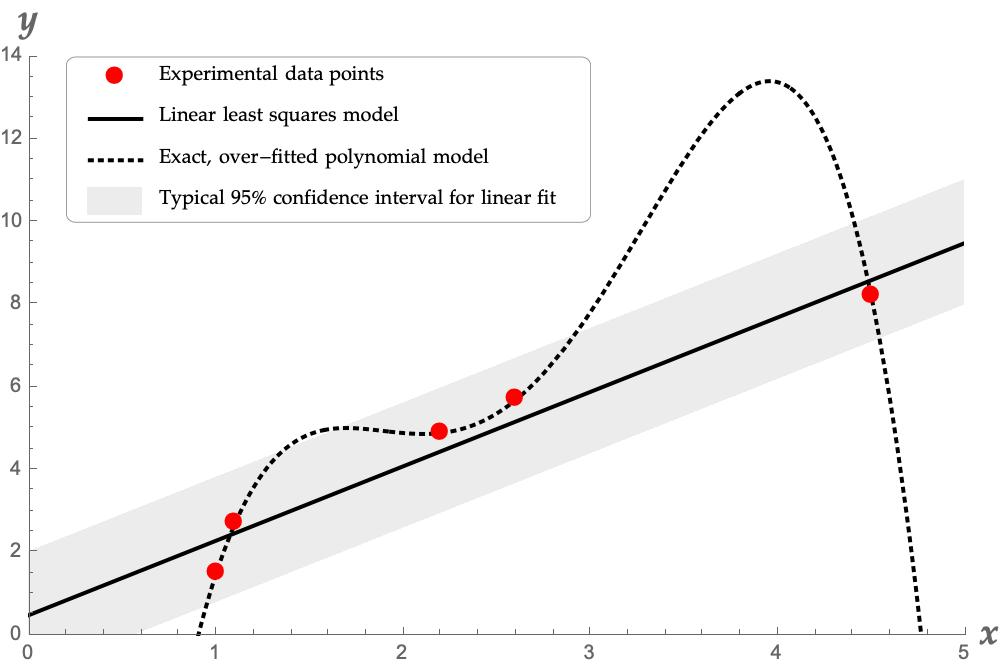
\includegraphics[width=\imageWidth]{
generated/mathematicaplot.jpg
}\end{center}}
\caption{Much computational science is concerned with finding plausible multi-dimensional models that fit models to data with the aim of extrapolating or predicting new results from them. Shown here is notional sample of experimental 2D data (the dots), a linear least squares regression, and an exact polynomial model. The over-fitted polynomial model fits the sample \emph{exactly\/}, but since the experimental data is presumably subject to random error (indicated by the confidence interval, itself estimated) the linear model would generally be considered a better description of the experimental data.}
\label{fig-overfit}
\end{figure\figureStarDetails}

In conventional modeling terms, successful computer programs are often \emph{over-fitted\/} to phenomena \cite{over-fit}. That is, instead of using code to rigorously challenge, test, and develop our models, we tinker with code adapting it to generate results closer and closer to our prejudices. The code then apparently confirms our science, since we fitted it to our preconceptions but not to the science.  

In general, an \emph{over-fitted model\/} fits a set of data closely, but contains more parameters than can be justified by the science. An over-fitted model fails to reliably predict results beyond the scope of the data it has been fitted to. Over-fitting is a well-known problem, but the point is that when code is used, over-fitting is done unconsciously by programmers adjusting the code --- its parameters, its structure, its embedded data, the calculations it performs --- that specifies the model. ``A model over-fits if it is  more complex than another model that fits equally well'' \cite{over-fit}, is a criterion that describes almost every program! Programmers without the discipline and experience to manage the unlimited adaptability of code debug, alter, and extend their code to make it do what they think it should do. This becomes a vicious circle as the idea of what the science is becomes driven by the code. Rather than debugging code by improving its fit to the actual science, it gets debugged and extended to fit the expectations.  

The problems of over-fitting data may be visualized using a Real$\rightarrow$Real function of one variable (figure \ref{fig-overfit}). The code that generates an over-fitted curve seems to work very well: in the example shown, the over-fitted curve fits the sampled data exactly; indeed, the code used here will fit any new data exactly as well. But the code has a negligible ability to predict new data or to describe theories of the data, which is the point of modeling. The fact that over-fitted code seems to work well is deceptive.

Looking specifically at the data plotted in figure \ref{fig-overfit} if, for the sake of argument, we assume the error in the data is normally distributed then the values the over-fitted code generates outside the range of the sample are improbable. For example, the basic linear model predicts
$\hat{y}(0)=0.5$, 
versus the extreme value predicted by the over-fitting code, 
$\hat{y}(0)=-41.8$, 
 even lies far outside the plot region shown in the figure.\footnote{The bounds of the confidence interval illustrated in figure \ref{fig-overfit} depend on assumptions about the distribution of the data; in this example, we are \emph{assuming}, perhaps because we know something more about the experiment, or thanks to Occam's Razor that a linear function is more likely than a high order polynomial.} Similar problems happen with interpolation rather than extrapolation, for instance around $x=4$.

While over-fitting data is a well-known problem, the point for this paper is that \emph{code\/} itself can easily be over-fitted. Code can of course be over-fitted in more complex ways than can be illustrated with elementary polynomials, as here. Code over-fitting is much harder to recognize because there may be no simple graph plot, like figure \ref{fig-overfit}, to highlight the problems. Furthermore, almost all code is far more intricate than the two trivial polynomials used to illustrated figure \ref{fig-overfit}. 

Unfortunately, code in published science \emph{is\/} often over-fitted, and over-fitted in a way that is very hard to scrutinize. For example, in epidemiology (which is considered in section \ref{section-pandemic-modeling}) it is routine to use very complicated, large dynamical models parameterized with numerous social, cultural, health, demographic and geographical data. The parameterization is mixed between data files, data written explicitly into the code, and with conditionals and other structuring in the code to cover special cases. Indeed, many of the programs in the survey used comments to inactivate code, presumably indicating an unfinished tinkering approach to code development.\footnote{Of the \the\countUsesVersionControlRepository\ papers in the pilot survey that reported use of code repositories (covering % expand generated/kloc.tex
\def\totalkLOC{182}%
% end expanding generated/kloc.tex
\totalkLOC\ thousand lines of code --- so this is not a trivial amount of programming effort), \numbertoname{\the\countMissingCode} provided an empty repository with no code at all (effectively commenting out all their code!), and \numbertoname{\the\countCommentedOut} repositories explicitly commented out chunks of workable code. The \numbertoname{\the\countNotCommentedOut} remaining non-trivial repositories with no commented-out code consisted of straightforward, short code files with few comments of any sort.\label{name-example-footnote}}

Furthermore, scientific support code is rarely documented well enough to know what it should have been doing, which should be answered by a specification. With no clear specification and documentation, the code can be arbitrarily hacked to get any convenient results, since no particular specification for it has been defined that it should adhere to. Thus we risk doing and promoting substandard science because we --- the scientists and the publication process --- are not managing the unlimited adaptability and complexity of code that science has come to rely~on. This is over-fitting of the worst kind --- in conventional over-fitting one can at least hope to see that the fitting is over-parameterized for the data, but in code over-fitting the code and specification are not visible, therefore not adequately scrutinized, and --- worse --- the ``data'' the code over-fits includes the entire conceptual contribution of the paper. 

Reference \cite{may-simple} shows that even trivial code (in the case cited, implementing simple difference equations) with very few parameters can have very complex results, and reference \cite{dyson} is a historically significant paper pointing out how the problems of over-fitting has improved science.
% end expanding generated/over-fitting-code-section.tex

\section{The conventional role of code}

Models map theory and parameters to describe phenomena, typically to make predictions, or to test and refine the theory supporting the models. With the possible exception of theoretical research, all but the simplest models require computers to use; indeed even theoretical mathematics is now routinely performed by computer.

Whereas the mathematical form of a model may be concise and readily explained, even a basic computational representation of a model can easily run to thousands of lines of code, and its parameters --- its data --- may also be extensive. The chance that a thousand lines of code is error free is negligible, and therefore good practice demands that checks and constraints should be applied to improve its reliability. How to do this is the concern of Software Engineering. 

While scientific research may rely on relatively easily-scrutinized mathematical models, or models that seem in principle easy to mathematize, the models that are run on computers to obtain the results published are sometimes not disclosed, and even when they are they are long, complex, inscrutable and (as our survey shows) lack adequate documentation. Therefore the models are very likely to be unreliable \emph{in principle}. 

If code is not well-documented, this is not only a problem for reviewers and scientists reading the research to understand the intention of the code, but it also causes problems for the original researchers themselves: how can they understand their historical thinking well enough (say, just a few weeks or months later) to maintain it correctly if it has not been clearly documented? As a scientist pursues a research career building on their previous work, how can they be certain their work is reliable, and not merely converging to their  prejudices? Without proper documentation, including a reasoned case to assure that the approach taken is appropriate \cite{assurance-case}, how do researchers, let alone reviewers, know exactly what they are doing?

Without substantial documentation it is impossible to scrutinize code properly. Consider just the single line ``\texttt{y = k*exp(x)}'' where there can be \emph{no\/} concept of its correctness \emph{unless\/} there is also an explicitly stated relation between the code and the mathematical specifications. What does it mean? What does \texttt{k} mean --- is it a basic constant or the result of some previous complex calculation? Does the code mean what was intended? What are the assumptions on \texttt{k}, \texttt{x}, and \texttt{y}, and do they hold invariantly? Moreover, as code generally consists of thousands of such lines, with numerous inter-dependencies, plus calling on many complex libraries of support code, it is inevitable that the \emph{collective\/} meaning will be unknown. A good programer would (in the example here) at least check that \texttt{k} and \texttt{x} are in range and that \texttt{k*exp} was behaving as expected (e.g., in case of under- or overflow).

Without explicit links to the relevant models (typically mathematics), it is impossible to reason whether any code is correct, and in turn it is impossible to scientifically scrutinize results obtained from using the code. Not providing code and documentation, providing partial code, or providing code without the associated reasoning is analogous to claiming ``statistical results are significant'' without any discussion of the relevant methods and statistical details that justify making such a claim. If such an unjustified pseudo-statistical claim was made in a scientific paper, a reviewer would be justified in asking whether a competent experiment had even been performed. It would be generous to ask the author to provide the missing details so the paper could be better reviewed on resubmission. 

Some authors assert that the purpose of code is to provide insight into models, rather than precise (generally numerical) analyses summarizing data or properties of the data \cite{assessing-quality}. In reality, if code is inadequate, any so-called ``insights'' will be potentially flawed, and flawed in unknown ways. Indeed, none of the papers sampled (see \supplement\ section~\ref{supplement-survey-section}) claimed their papers were using code for insight; all papers claimed, explicitly or implicitly, that their code outputs were integral to their peer-reviewed results.

Clearly, like statistics, coding can be done poorly and reported poorly, or it can be done well and reported well --- and any mix between the extremes. The question is whether it matters, \emph{when\/} it matters, and, if so, when it does, \emph{what\/} can be done to \emph{appropriately\/} help improve the quality of code (and discussions about the code) in scientific work?

\subsection{The deceptive simplicity of code}\label{deceptive-simplicity-of-code}
It is a misconception that programming is easy and even children can do it \cite{fixit}. More correctly, toy programming is easy, but mature programming is very difficult. % (compare: ``brain surgery is very easy and anybody can do it, but it is very hard and hardly anyone can do it if you require the procedure to be successful'').

An analogy helps justify this key point. Building houses is very easy --- indeed, many of us have built toy Lego houses. Obviously, though, a Lego house is not a \emph{real\/} house. It is not large enough or strong enough for safe human habitation! This point is obvious because we can see Lego houses, and everyone is familiar with the limitations of building-block play. Its real-world engineering limitations are too obvious to need stating. 

In contrast to Lego, computer programs are generally invisible, and therefore the engineering problems within them are also made invisible. The ``programming is easy'' clich\' e is deceptive --- programming appears easy \emph{because\/} professional standards of building software are ignored, because people cannot see the reasons why they are needed, and because --- like Lego --- toy programs can look inspiring but be unreliable, difficult to use, even dangerous. 

Saying programming is easy is like appreciating a child's Lego building because we are not worried about subsidence, load bearing, electric shock, fire risks, water ingress, or even planning regulations. These are professional engineering issues that Lego builders ignore. Certainly, even real building is much easier and faster when the technical details are ignored, as anyone who has experienced a cowboy builder can attest.

Unlike building houses (the Code of Hammurabi dates from around 1755\hskip .2em{\sc bc}\footnote{The Code of Hammurabi says, ``(\S 233) If a builder constructs a house [and] does not make it according to specifications, and a wall then buckles, that builder shall make that wall sound using his own silver.'' \cite{Hammurabi}}), programming is a new discipline, and the problems of poor programming are not widely appreciated or embedded in our culture. Professional standards, even when they exist, are not enforced. 

Problems for the reliability of science arise when doodling and tweaking software drifts into claiming scientific results that do not have reliable engineering processes or structures underpinning them (let alone the properly developed and documented accessible code) to justify them. 

In many countries, there are laws that require all but the very simplest building structures to be formally approved from plans and inspected as they are built, but who writes plans for software, who inspects scientific models while they are being coded? Yet the consequences of building a shoddy garage have negligible impact compared to the consequences of writing poor code that informs national public health policies or climate change interventions.

\subsection{The low status of coding}\label{lowCodeStatus}
Since programming appears to be so easy, developing code has a correspondingly low status in scientific practice (and more widely). Developers of code are rarely acknowledged in scientific papers. The implicit reasoning is: if programming is easy, then its intellectual contribution to science is negligible, so it is not even worth citing it or acknowledging the contributors to it. Because it is apparently easy, there is no need to work hard to make it correct. Because of the ease of over-fitting (section \ref{over-fit}), code ``works well'' with little skill or effort. While such mistaken views prevail, the vicious cycle is that the low status means software development is casualized, which reinforces the low status.

Almost all scientific papers \emph{routinely\/} describe their experimental method, their data handling, and provide an overview of their analytic (usually statistical) methods. If they are theoretical papers, they will describe their mathematical models and data that is used to run or test their models. However, outside of pure computer science, scientific papers are almost entirely silent on the code they rely on and how it was developed --- in particular, how the code might have been protected from bugs, analogously to how appropriate experimental methods were used avoid or control for experimental error. 

%An example is the documentation at the code repository \xcite{BayesWaveCode}, which requires three high-profile \emph{{Physics Review D}} papers \xcite{BayesWave1,BayesWave2,BayesWave3} be cited to acknowledge any use, but only one of them, \xcite{BayesWave3}, mentions the code, and even then it fails to acknowledge the contributions of its 10 programmers (despite 6 being co-authors). The paper does cite the repository URL, but unlike the papers it cites conventionally, it omits all the code's authors. Acknowledgement does not seem to matter, even to the people who did the work.

Since published papers rarely mention their code, new papers contributing to the literature do not write about their code either, so the low status of code persists. 

In reaction to this vicious cycle, there is a growing movement to use and cite code correctly \cite{cite-code,TOP}, because code \emph{is\/} important, particularly for the reproduction, testing, and extension of any scientific work. (Code also needs to be correct, not just cited correctly.)

%Few journals editorial policies recognize that data and code are theoretically and in practice indistinguishable (see \supplement). Given that data and code are equivalent and interchangeable, it follows that publishing policies on data handling should also apply at least as strictly to code.

\subsection{The critical role of code is often ignored}\label{central-role-of-code}\label{PRISMA-statement}
Because statistics, like code, is so readily susceptible to uncontrolled bias and error, there are many protocols and journal policies that enforce best practice, for example journals often require adherence to PRISMA (Preferred Reporting Items for Systematic Reviews and Meta-Analyses) \cite{prisma} for any paper performing a systematic review of the literature. PRISMA is a leading and influential research protocol, and it serves to make the point that the critical role of code is often strategically ignored. 

PRISMA is not concerned with the reproducibility of the literature reviewed, nor the reproducibility of systematic reviews themselves. PRISMA not only ignores the role of code, it ignores the Software Engineering principles that assure code that research relies on is reliable and reliably reported. 

PRISMA covers the review workflow. For example, it states that authors should report the number of papers they included in their review. Perhaps $N=2\hskip 0.3em 000$. This number will then written be into the review, perhaps in several places. As the authors read and revise their paper and respond to peer-reviewers, it is likely that the number of papers in the survey will change; other numbers and details will certainly change. 

The authors now have a maintenance problem that PRISMA does not address: where are the numbers that have changed, and what should they be changed to? Doing a search-and-replace, whether automated or by hand, is fraught with difficulties. What happens if $2000$ is used for some other purposes as well? What happens if some of the $2000$ values are written as $2,000$ or as $2\hskip 0.3em 000.0$, or if a number containing the digits 2000, like 12000, is changed? What happens if some $2000$ are year dates and are changed incorrectly? 

Then there are the Human Factors: slips and errors will happen in this workflow anyway \cite{engima}. Typos, slips during cut-and-paste, and other errors are common. Similar iterative revision cycles happen with any paper, not just with systematic reviews. 

PRISMA, like many such standards, ignores the methodological problems of using code such as the issues raised above. 

The irony, then, is that PRISMA says nothing about how to ensure the results of a survey are correctly and reliably presented, despite this being one of PRISMA's explicit motivations. PRISMA explicitly warns about methodological issues, but ignores that poorly managed code raises methodological issues that will undermine the validity of research it supports. PRISMA reinforces the culture that code is trivial and incidental to research.

\subsection{Bugs, code and programming}\label{knowledge}
Critiques of data and model assumptions are increasingly common \cite{critiques,diagnosis-reviews} but program code is rarely mentioned. Program code has as great an effect on results as the data; in fact, without code, the data would be uninterpreted and almost useless. Code, however, is harder to scrutinize, which means that errors in code have subtle, often unnoticed effects on results.

Program code contains data. Almost all code contains ``magic numbers'' --- that is, data masquerading as code (see \supplement, section \ref{supplement-on-code-data-publication}). This common practice ensures that published data is rarely all of the relevant data because it omits the magic numbers embedded in the code. Such issues emphasize the need for repositories to require the inclusion of code so all data, including that embedded in the code, is actually available. 

Conversely, much data contains code. Excel spreadsheets are often used to manage code, and almost all Excel spreadsheets contain macros and formul\ae\ --- code embedded in the data. JSON, the JavaScript Object Notation, is a structured data language, but as it is part of the JavaScript programming language there is no practical code/data distinction. Indeed, the present paper's data is in a file \texttt{data.js} that also contains the JavaScript code to analyze it and generate results (such as Table \ref{table-summary}) for presentation in this paper.

Although convenience and convention treat data and code differently, ultimately, data and code are formally equivalent (see \supplement, section \ref{supplement-on-code-data-publication}) in the important sense that there is no pre-determined boundary between them or formal criteria to distinguish them: different scientific projects can draw their boundaries differently and as they see best fits their work. Indeed, all of the papers reviewed here where code was available include critical data in their code. It therefore makes no sense to have separate rules for data and code --- except in the most trivial cases \emph{both\/} are equally essential for verification, building on, and reproduction of work. 

Bugs can be understood as discrepancies between what code ought to do and what it actually does. Many bugs cause erroneous results, but bugs may be ``fail safe'' by causing a program to crash so no incorrect result can be delivered. Contracts and assertions are essential defensive programming technique that block compilation or block execution with incorrect results; they turn bugs into safe termination, or, better, failure to compile. None of the science surveyed in this paper includes any such basic techniques. 

Random numbers are widely used in computational science (and in many of the papers surveyed), for simulation or for randomizing experiments. Misuse of random numbers (e.g., using standard libraries without testing them) is a very common cause of nai\"\i ve bugs \cite{knuth}.

If code is not documented it cannot be clear what it is intended to do, so it is not possible to detect and eliminate bugs. Indeed, even with good documentation, \emph{intentional bugs\/} will remain, that is, code that correctly implements the wrong things \cite{essence-of-software,fixit}. Intentional bugs occur in code that correctly does what was intended, but what was intended was itself faulty (students and inexperienced programmers regularly make intentional bugs). Intentional bugs frequently arise in numerical modeling, where using an inappropriate method can introduce errors that are not bugs in the sense of failing to correctly implement what was wanted, but are bugs in the sense that the wrong numerical method was chosen and inaccurate results are obtained; that is, what was intended was~wrong. 

\subsection{Long-term problems of unreliable code}
Scientists explore and extend the boundaries of rigorous knowledge. Put briefly, the purpose of scientific experiments is to vary details to either test and specify the boundaries of theories, or to discover new phenomena that then lead to theory revision. 

If poor code, or poorly documented code, is made available with scientific papers, the code is a natural place to start replicating and varying experimental conditions, including both data or code. However, if the starting point is not accurately known, whether due to bugs, obscure code, or because of poor documentation, then experimental variations will have an unknown effect. Theory will then be driven by artifacts of the code, not genuine phenomena. 

In section \ref{section-pandemic-modeling}, below, an example is documented of a research code development process of at least 15 years' duration where the code was admitted to be completely undocumented, leaving details in just one author's head. None of the various related papers describe any controls over the drift of the science, or how independent researchers building on it might have been able to build with confidence rather than merely reproducing the same errors. 

Since the code in question was substantial and non-trivial, it is very unlikely that any constructive reproduction occurred outside the original laboratory and mindset; indeed, section \ref{reproducibility-concerns} describes how ``reproduction'' became trivialized because of community pressure to confirm the insights of this particular research. 

Trying to constructively refute aspects of this research in the Popperian sense \cite{popper-conjectures-refutations} would have been impossible. For example, had the relevant papers published critical code invariants then scientists building on the research could have explored whether those invariants remained valid and, if so, under what assumptions. In fact, invariants are the theories of code, and deserve as high a prominence in published  science as the domain theories the code itself is supporting investigating. 

%Since the symmetries in the scientific domains should be reflected in corresponding symmetries in well-designed code, this raises new possibilities of Formal Methods approaches (e.g., using automatic theorem provers) supporting advances in general science.

\section{State of the art}% \\ in computational science}

\subsection{Case study: Pandemic modeling}
\label{section-pandemic-modeling}
For an excellent review of the extreme pressures under which scientists were working during the COVID-19 pandemic (but nothing about the role of computers!), see \cite{preventable-book} --- which, while referring to some failed mRNA vaccines, makes an important point on recovering from ``failed'' science:

\begin{quote}\raggedright
{\sf\setbox0=\hbox{``}
\hskip -\wd0\box0
Such is the beauty of science: even failed attempts are a step towards more information and progress forward.''} \cite{preventable-book}
\end{quote}

But progress, if any, would be chaotic if it was not possible to scrutinize exactly what science has failed. It undermines progress if science and the code it relies on are not both accessible and adequately defined. It is as misleading as getting the statistics or mathematics wrong.

By focusing on influential science and coding undertaken to inform public health policies during a pandemic emergency, this section now focuses on an area where reliable and high quality science using code open to interdisciplinary scrutiny was very obviously required. Note that pandemic model correctness is a secondary concern here; correctness is not addressed as without informed scrutiny correctness cannot even be assessed. 

A review of epidemic modeling \cite{science-review} says, ``we use the words `computational modeling' loosely,'' and then, curiously, the review discusses exclusively mathematical modeling, implying that for the authors, and for the peer-reviewers, there is no role for code or computation as such. It appears that the new insights, advances, rigor, and problems that computers bring to research were not considered relevant. 

A systematic review \cite{diagnosis-reviews} of published COVID-19 models for individual diagnosis and prognosis in clinical care, including apps and online tools, noted the common failure to follow standard TRIPOD guidelines \cite{tripod}. The review \cite{diagnosis-reviews} itself ignored the mapping from models to their implementation, yet if code is unreliable, the model \emph{cannot\/} be reliably used, and cannot be reliably interpreted regardless of whether TRIPOD guidelines are followed. Indeed, TRIPOD guidelines ignore code completely. 

It should be noted that flowcharts, which the review \cite{diagnosis-reviews} did consider, are graphical programs intended for human use. Flowcharts, too, should be designed as carefully as code, for exactly the same reasons. 

A high-profile 2020 COVID-19 model \cite{nature-summary,ICmodel}, which influenced UK COVID-19 public health strategies, uses a modified 2005 computer program \cite{avianFluModel,originalICmodel} originally developed for modeling H5N1 in Thailand, when it did not model air travel or other factors required for later western COVID-19 modeling. The 2020 model forms part of a series of papers \cite{ICmodel,avianFluModel,originalICmodel} none of which provide details of their code. 

A co-author disclosed \cite{tweet} that the code was thousands of lines long and was undocumented code. As Ferguson, the original code author, noted in an interview, 

\begin{quote}\raggedright
{\sf\setbox0=\hbox{``}
\hskip -\wd0\box0 
For me the code is not a mess, but it's all in my head, completely undocumented. Nobody would be able to use it~\ldots
''} \cite{ferguson-interview}\end{quote}

The admission above is tantamount to saying that the published scientific findings are and need not be reproducible.\footnote{A constructive discussion of Software Engineering approaches to reproducibility can be found in \cite{basic-reproducibilty}.} 

The comment was made by a respected, influential world-leading scientist, with many peer-reviewed publications involving computational modeling, with a respectable $h$-index\footnote{$h$-index: the largest value of $h$ such that at least $h$ papers by the author have each been cited at least $h$ times. The figure cited for Ferguson was obtained from Google Scholar on 20 January 2022. (Typical $h$ values vary by discipline.)} of 93, and at the time ``one of the top scientists advising the government on its response to the coronavirus crisis'' working in the UK's Scientific Advisory Group for Emergencies (SAGE) group \cite{ferguson-resign}. 

Ferguson's code must be representative of best practice when the stakes were high and reliability was known to be essential; and if not representative of best practice, at least representative of accepted practice both in Ferguson's team, the field of epidemiology more widely, as well as with members of the high-powered interdisciplinary SAGE group. It is therefore instructive to explore the larger story around this science that uses code. 

Lack of reproducibility is problematic, especially as the model code would have required many non-trivial modifications to update it for COVID-19 with its different assumptions; moreover, the code would have had to have been updated very rapidly in response to the urgent COVID-19 crisis. 

If Ferguson's C code had been made available for review, the reviewers would not have known how to evaluate it without the relevant documentation. It is, in fact, hard to imagine how a large undocumented program could have been repeatedly modified and repurposed over fifteen years without becoming incoherent. 

If code is undocumented, there would be an understandable temptation to modify it arbitrarily to get desired results (i.e., over-fitting, see section \ref{over-fit}); worse, without documentation and proper commenting, it is methodologically impossible to distinguish legitimate attempts at debugging from merely fudging the results. In contrast, if code is properly documented, the documentation defines the original intentions (including, where appropriate, formally using mathematics to do so), and therefore any modifications will need to be justified and explained --- or the theory revised.

The programming language C which was used \cite{tweet} is, like many popular programming languages, not a dependable language; to develop reliable code in C requires professional tools and skills. Some of the code was written in a na\"\i ve style (e.g., writing \texttt{*(a + i)} instead of \texttt{a[i]}, and with obscure numerical goto statements like \texttt{if(l == 0) goto S150}), and with C code that was translated simplistically from FORTRAN and Pascal code, from references dating back to the 1970s and 1980s \citeeg{forsyth,Normal-Distributions}.

Moreover, C code is not portable, which limits making it available for other scientists to use reliably: C notoriously gets different results with different compilers, libraries, or hardware. In fact, in any area where reliable programming is required in a C-like language, a special dialect such as MISRA C is preferred: MISRA C manages the serious design flaws of C that otherwise make it too unreliable \cite{misra}. Alternatively, a high integrity programming language, unrelated to C, such as SPARK Ada \cite{spark}, or modern languages (many related to the ``ML family'') like OCaml, F*, Haskell \cite{haskell} could be used. These languages have steeper learning curves; however their key benefit is that correct programs are far more likely and are \emph{much\/} faster to write. (The \supplement\ discusses these issues further.) 

Ferguson, author of the code, says of the criticisms of his code, 

\begin{quote}\raggedright
{\sf\setbox0=\hbox{``}
\hskip -\wd0\box0 
However, none of the criticisms of the code affects the mathematics or science of the simulation.''} \cite{thumbs-up}
\end{quote}

This claim is implausible. 

The original work on theoretical epidemiology may be fine if it does not use any of his code, but if the science is not supported by code that correctly implements the models, then the program's output cannot be relied on without independent evidence. Over the fifteen plus years the code was in development the science it informs will have developed too, as will the relevant data; it is not clear how they will have remained in alignment.

\label{discuss-covid-sim}
Typically, models will be developed iteratively as their results are improved to better fit a scientist's goals --- but this, especially when it is done by tinkering, as here --- risks making the code arbitrarily fit the goals (that is, over-fitting; see section \ref{over-fit}), rather than to objectively elucidate the science. 

In fact, the Ferguson code, \texttt{covid-sim}, is a very large program at \covidsimkLOC\ kLOC (thousands of lines of code),\footnote{Ferguson's \texttt{covid-sim} system is composed of \covidsimfiles\ files, and uses \covidsimdata\ of data. It is now rewritten from C into C++ with Python, R, sh, YAML/JSON, etc. For more details, see \supplement.} so it is implausible that the ``mathematics or science'' has been correctly implemented in it without error, particularly as there is no discussion of methodologies to code reliably. Ferguson's \emph{reported\/} science is consequently unlikely to be reliable. 

\subsection{Concerns with reproducibility}
\label{reproducibility-concerns}
Getting science right, which now, in turn, depends on correct code, is a normal requirement of \emph{reproducibility}.

The code in \cite{nature-summary,ICmodel} has been ``reproduced,'' as reported in \emph{Nature\/} \cite{codecheck,thumbs-up}, but this so-called reproduction merely confirms that the code can be run again and produce comparable results. As Eglen says,

\begin{quote}\raggedright
{\sf\setbox0=\hbox{``}
\hskip -\wd0\box0 Each run generated a tab-delimited file in the output folder. Two R scripts provided by Prof Ferguson were used to summarise these runs into two summary files [\ldots] These files were compared against the values generated by Prof Ferguson [\ldots] The results were found to be identical. Inserting my results into his Excel spreadsheet generated the same pivot tables. The codecheck found that: `Small variations (mostly under 5\%) in the numbers were observed [\ldots]'\,''} \cite{codecheck}
\end{quote}

This test would pass provided the runs gave the same answers regardless of whether the answers are correct --- it is not a usefully stronger test than just checking that the code compiles. The comparison relied on running (apparently) unchecked R code to summarize the data, which is potentially misleading unless the published results \cite{ICmodel} exclusively relied on the same summary code. In general, reproducing code results, even done formally, does not scrutinize the science, as  \cite{codecheck-certificate} makes clear.

Running code just to obtain results claimed in a paper is a weak test, and anyway one that should be checked routinely during paper preparation and submission. However, in this case the reproduction involved a community effort that also refactored and improved the code, which added value to the code and usefully improved its generality \cite{codecheck}. The reproduction effort was also certified \cite{codecheck-certificate}, which is the sort of evidence of quality assurance processes that arguably should be required before publication, particularly for critical code such as public health modeling. The publicity of this story and the certificate will certainly raise the profile of the scientific value of independent review of code. 

Unfortunately, the terms reproducibility, replicability, and repeatability, have similar meanings in English but have been used in different specific technical ways by different authors. In \cite{codecheck,thumbs-up} the reproduction amounted to just re-running the original code. It is certainly essential to establish that a paper's code can be run, as non-working code cannot support any claims in a paper; if the original code runs this confirms a basic level of access for the wider scientific community, and this can be formally certified \cite{codecheck-certificate} so it is appreciated by the community. But a more realistic criterion than basic reproduction in this sense is whether an \emph{independently\/} developed model developed from the same paper(s) specifications produces equivalent results (called $N$-version programming, a standard Software Engineering practice \cite{NVP}) like public health surely requires as, indeed, Ferguson's own influenza paper \cite{nvp-ferguson} argues. 

In general, much stronger scrutiny of code than ``reproduction'' is required to answer essential questions (numbered below for reference) including:

\newcount \enum
\enum=1
\renewcommand{\theenumi}{\ifnum \enum<10 \hphantom{0}\fi
\the\enum
\global\advance \enum by 1}
\begin{enumerate}\raggedright
\item Is the code valid: does it do what the paper claims?\footnote{Of course, the underlying science may be wrong to, so it is useful to distinguish \emph{internal validity\/} and \emph{external validity}. Internal validity occurs if the code does what the paper claims; external validity occurs if the code represents correct science which the paper may have interpreted incorrectly.}
\item Do other scientists, including reviewers and the authors, understand the code?
\item Does the code implement the methods described in the paper?
\item Has the code been over-fitted or tweaked to support specific claims in the paper?
\item Is there a definitive version of code?
\item Is the code controlled and signed?
\item What limitations does the code have?
\item Was the code developed to any standard, and does it comply to that standard?
\item How does the code protect against data, coding, and human error?
\item Was the code tested adequately?
\item Does the code depend on arbitrary parameters, data, or code to over-fit to obtain the published results?
\item Is the code documented adequately, so we know what it is trying to do, and how?
\item \ldots\ and so forth. 
\end{enumerate}

All such questions also apply to specifications, documentation, assurance cases, test procedures, and other essential documents, not just to code. In turn, the levels of scrutiny demanded should be guided by explicit claims in the paper \cite{essence-of-software} --- for example, a pilot study requires weaker assurance than code that is developed concerning nuclear power, driverless vehicles, public health, etc. 

The questions in the list above are certainly hard to answer for all but the briefest code, but corresponding levels of quality assurance are demanded for other methodologies \cite{notebooks,popper-conjectures-refutations,tripod,prisma,nih-policy,nih-nature}, such as data preparation and statistics to support claims in peer-reviewed science. 

Because of the recognized importance of the Ferguson paper, a project started to document its code  \cite{refactoring}.\footnote{It is surprising to find an undocumented model being used in the first place, since so many years' opportunity to improve the code have been lost. The revised code has now been published, and it too has been heavily criticized \citeeg{bad-code}, supporting the concerns expressed in the present paper.
n-source, available at \url{github.com/mrc-ide/covid-sim} version (19 July 2021).} Documenting code in hindsight, even if done rigorously, may describe what it does, \emph{including\/} its bugs, but it is unlikely to explain what it was originally intended to have done. As the code is documented, bugs will be found, which will then be fixed (refactoring), and so the belatedly-documented code will not be the code that was used in the published models; it will be different. 

It is well-known that documenting code helps improve it, so it is surprising to find an undocumented model being used in the first place, since so many years' opportunity to improve the code have been lost. The revised code has now been published, and it too has been heavily criticized \citeeg{bad-code}, supporting the concerns expressed in the present paper.

Some papers \citeeg{pseudo} publish models in pseudo-code, a simplified form of programming. Pseudo-code looks deceptively like real code that might be copied to try to reproduce it, but pseudo-code introduces invisible and unknown simplifications. Pseudo-code, properly used, can give a helpful impression of the overall approach of an algorithm, certainly, but pseudo-code alone is not a surrogate for code: using it instead of making actual code available is worse than not publishing code at all (see \cite{chinese}). Pseudo-code is too vague to help anyone scrutinize a model; moreover, pseudo-code may mask over-fitting in code used that is not explicit in the pseudo-code. 

An extensive criticism of pseudo-code, and discussion of tools for reliable publication of code can be found elsewhere \cite{relit}. 

The \supplement\ provides further discussion of reproducibility.

\subsection{Beyond pandemic modeling}
\label{section-science-beyond-pandemic-modeling}

Epidemiology has a high profile because of the COVID-19 pandemic, but the problems of unreliable code are not limited to COVID-19 modeling papers, which, understandably, were perhaps rushed into publication. But other examples that were not rushed include a 2009 paper reporting a model of H5N1 pandemic mitigation strategies \cite{flu-model}, which provides no details of its code. Its supplementary material, which might have provided code, no longer exists.

There are many other areas of computational science that are equally if not more critical, and many will have longer-lasting impact. Climate change modeling is one such example that will have an impact long beyond the COVID-19 pandemic.

A short 2022 summary of typical problems of Software Engineering impacting science appears in \emph{Nature\/} \cite{nature-review}, describing diverse and sometimes persistent problems encountered during research in cognitive neuroscience, psychology, chemistry, nuclear magnetic resonance, mechanical and aerospace engineering, genomics, oceanography, and in migration. The paper \cite{nature-review}  makes some misleading comments about the simplicity of Software Engineering, e.g., ``If code cannot be bug-free, it can at least be developed so that any bugs are relatively easy to find.''

Guest and Martin promote the use of computational modeling \cite{psychological-modeling}, arguing that through writing code, one debugs scientific thinking. Psychology, their focus, has an interesting relationship with software, as computational models are often used to model cognition and to compare results with human (or animal) experiments \cite{psychological-modeling}. In this field, the computation does not just generate results, but is used to explicitly explore the assumptions and structures of the scientific frameworks from which the models are derived. Computational models can be used to perform experiments that would be unethical on live participants, for instance involving lesioning (damaging) artificial neural networks. It should be noted that such use of cognitive models is controversial --- on the one hand, the software allows experiments to be (apparently) precisely specified and reproduced, but on the other hand in their quest for psychological realism the models themselves have become very complex and it is no longer clear what the science is precisely!

For instance, ACT-R, one widely-used theory for simulating and understanding human cognition, has been under development since 1973, and is now a 120 kLOC Common LISP and Python system \cite{actr}. Furthermore, any paper using ACT-R would require additional code on top of the basic ACT-R framework.

The psychology paper \cite{psychological-modeling} presents an example computational model from scratch to illustrate a framework of computational science. In fact their example model has no psychological content: a simple numerical test is performed, but the psychology of why the result is counterintuitive --- the psychological content --- is not modeled. Be that as it may, they develop a mathematical specification and discuss a short Python program they claim implements it. 

The Python code is presented without derivation; Software Engineering is ignored. The program listed in the paper certainly runs without obvious problems (ignoring some typographical errors due to the journal's publishers), but ironically the Python does \emph{not\/} implement the mathematical specification explicitly provided for it, thus undermining the argument of the~paper. 

One might argue the bug is trivial (the program prints \texttt{False} when it should print \texttt{b}), but to dismiss such a bug would be comparable to dismissing a statistical error that says $p=\mbox{\tt False}$ which would be nonsense --- if a program printed that, one would be justified in suspecting the quality of the entire program and its analyses. Inadvertently, it would seem, then, that the paper shows that just writing code does not help debug scientific thinking: instead, code must first be derived in a rigorous way and actually be correct. Otherwise, code based on inadequate Software Engineering will introduce errors into scientific thinking.

Code generally for any field of scientific modeling needs to be carefully documented and explained because all code has tacit assumptions, bugs and cybersecurity vulnerabilities \cite{Ben,nature-review,se-bias} that, if not articulated \emph{and properly managed}, can affect results in unknown ways that may undermine any claims. People reading the code will not know how to obtain results because they do not know exactly what was intended in the first place. The problem is analogous to the problem of failing to elaborate statistical claims properly: failure to do so suggests that the claims may have unknown limitations or flaws.

Even good quality code has, on average, a defect every 100 lines --- and {such a low} rate is only achieved by experienced industrial software developers \cite{ourReview}. World-class software can attain maybe 1 bug per 1,000 lines of code. Code developed for experimental research purposes will have higher rates of bugs than professional industrial software, because the code is less well-defined and evolves as the researchers gain new ``insights'' into their ideas, unable to distinguish genuine insights from artifacts of bugs. In addition, and perhaps more widely recognized, code --- especially but not exclusively mathematical code --- is subject to numerical errors \cite{hamming}. It is therefore inevitable that typical modeling code has many bugs (reference \cite{NVP} is a slightly-dated but very insightful discussion). Such bugs undermine confidence in model results. 

Only if there is access to the \emph{actual\/} code and data (in the specific version that was used for preparing the paper) does anyone know what the researchers have done and whether that corresponds closely to what they are reporting.

Some COVID-19 papers \citeeg{unfinished} make unfinished, incomplete code available. While some \citeeg{unfinished,lancet-unfinished} make what they call ``documented'' code available, they provide no more than superficial comments. This is \emph{not\/} documentation as properly understood. Such comments do not explain code, explain contracts, nor explain algorithms. Contracts, for instance, originated in work in the 1960s \cite{hoare}, and are now well-established practice in reliable programming.

Even if a computer can run it, badly-written code (as found in \emph{all\/} the research reviewed in the present paper, and indeed in computer science research, e.g., \cite{machine-learning-reproducibility}) is inscrutable. Only if there is access to \emph{adequate\/} documentation can anyone know what the researchers \emph{intended\/} to do. Without all three (code, data, adequate documentation), there are dangers that a paper simplifies or exaggerates the results reported, and that omissions, bugs and errors in the code or data, generally unnoticed by the paper's authors and reviewers, will have affected the results they report \cite{relit}. 

\label{section-discussion}
\subsection{The lop-sided emphasis on data}
\label{critique-fair}
Data has been at the center of science, certainly since the earliest days of astronomy collecting planetary and other information. Today it is widely recognized that lack of accessible and usable data that has already been collected limits the progress of science. Low quality data and poor access to data causes reproducibility problems, an increasingly recognized problem --- in 2015 it was estimated that \$28 billion a year is spent on preclinical research that is not reproducible \cite{preclinical-reproducibility}.

Curating data is taken seriously as a part of normal science and peer-reviewed publication. Journal policies widely require appropriate discussion of data, much as they require appropriate discussion of statistics. Journals often require archiving data in standard formats so it can be accessed for reproduction in further scientific work. 

There are many current activities to proceduralize and standardize the more effective curation and use of data, such as the FAIR principles (Findable, Accessible, Interoperable and Reusable) for scientific data management and stewardship \cite{fair,fair-principles}, and in the development of journal and national funder policies. For example, the 2022 update to the US National Institutes of Health data policies \cite{nih-policy} is described as a ``seismic mandate'' by \emph{Nature\/} \cite{nih-nature} in its attempt to improve reproducibility and open science yet they ignored code.

These cost estimates and initiatives under-play the role of code as a critical component despite its becoming the new laboratory for almost all science. The role of code specifically in modeling is discussed throughout this paper; without bespoke code, proposed models (unless intended to be abstract) cannot make a quantifiable contribution to the literature. Code has additional problems of versions and compatibility beyond those of data, for example suitable compilers to run old code may no longer be available, and  programming systems may produce different results when used on different computers. 

In general, without proper management of code --- for example to record, detect and report version control differences --- sharing code may even be counter-productive.\footnote{The data and code shared with the present paper includes cryptographic checksums; if somebody reproducing the work described here does not obtain the same checksums at least when they start their work, then there are problems that need investigation before relying on the reproducibility of the data.}

Using structured repositories that provide suggestions for and which encourage good practice (such as Dryad\footnote{Dryad \url{datadryad.org} curates raw, unprocessed data. At the time of writing, Dryad excludes code; however, it uses a separate organization, Zenodo \url{zenodo.org}, to host code and other relevant information. This arbitrary separation is unfortunate as it increases management problems, increases reproducibility problems, limits using RAP, and most seriously limits how scientists can structure their data and code to best suit their research (see section \ref{knowledge}).} and GitHub), and requiring their use, would be a lever to improve the quality and value of code and documentation in published papers. The evidence (see \supplement) suggests that, generally, some but rarely all develop code that is uploaded to a repository just before submitting the paper in order to ``go through the motions.'' In the surveyed papers there is no evidence (before, during, or after the date of the survey sample) that any published code was prepared or maintained \emph{using\/} repositories. This is consistent with the finished code being uploaded to a repository just for the purposes of satisfying publishing requirements, but not using one earlier probably because they did not understand the benefits of doing so --- not using a repository \emph{during\/} the research process means the author of the paper misses out on the many helpful features of repositories, such as version control, review, actions, and other approaches for automating development, sharing workload, and so on. Using repositories during research means that other people can more easily help review the approach, in much the same way that papers are routinely circulated for peer review before submitting to a formal journal.

There is a lop-sided emphasis on data in science. In fact, data is useless without code, and code must be used to manipulate and analyze it. Often code is used to extrapolate data, so the code itself effectively generates more data, or the code eliminates outliers so it effectively deletes data. Data is routinely formatted in simple or standard ways, but code, in contrast, is architecture- and version-specific, so --- unless properly managed --- code goes obsolete faster than data. In short: the integrity of code and its availability to scrutiny is in fact both harder and more important than the usual requirements put on data.

\section{Rethinking science that uses code}\label{summary}
Computer programs are the laboratories of modern scientists, and should be used with a comparable level of care that virologists use in their laboratories --- lab books and all \cite{notebooks} --- and for exactly the same reasons: bugs, whether computer bugs or biological bugs, accidentally cultured in one laboratory can infect research, ideas, and policy worldwide. 

Inadequate scientific code can be problematic. Incorrect results might be used for supporting science, modeling pandemics or informing public health policy, informing medical research, or adopted for use in other critical software, such as medical diagnostics, credit checking, or any other impactful use. Professional critical software development, as used in critical industries such as aviation and the nuclear power, is (put briefly) based on \emph{correct by construction\/} \cite{cbc}, effectively: design it right first time, supported by numerous rigorous techniques, such as Formal Methods, to manage error. Not coincidentally, these are \emph{exactly\/} the right methods to ensure code is both dependable and scrutable, as is required for supporting reproducibility and quality science more generally. Conversely, not following these practices undermines the rigor of science. 

\subsection{Software Engineering Boards}
Misuse of data, exploiting vulnerable people, and not obtaining informed consent are typical ethical problems. Planned research may be ethically unacceptable in ways the investigators do not anticipate: few people have the objectivity and ethical expertise to make sound ethical judgements, particularly when it comes to assessing their own work. National funders, and others, therefore require Ethics Boards to formally review ethical quality. Medical journals will not publish research that has not undergone independent formal ethical review. 

Analogously, and supplementing Ethics Boards, it is argued here that Software Engineering Boards (SEBs) would authorize as well as provide advice to guide the implementation of quality Software Engineering to support research and publication processes. Just as journals require conflicts of interest statements, data availability statements, and ethics board clearance, we should move to scientific papers and funded research being required to include formal Software Engineering Board statements. Note that Software Engineers themselves have a code of ethics that applies to their own work \cite{ethics-code}.

Some journals have policies that code is to be made available (see \supplement), but they should require that code is not just available in principle but \emph{actually works\/} on the relevant data. The authors should test a clean deployed build of their code and save the results. Presumably a paper's authors must have run their code successfully on \emph{some\/} data at least once, so preparing the code and data in a way that is reproducible should be a routine and uncontentious part of the rigorous development of code underpinning \emph{any\/} scientific claims. This requirement is no more unreasonable than requesting good statistics, as discussed earlier. And the solution is the same: that relevant experts --- statisticians or Software Engineers --- need to be available and engaged with the science. Software Engineering Board statements would be a straight forward way of helping achieve this and showing that it has been done adequately.

There need to be many SEBs to ensure convenient access, potentially at least one per university. Active, professional Software Engineers should be on these SEBs; this is not a job for people who are not qualified and experienced in the area or who are not actively connected with the state of the art. There are many high-quality university computer science departments and software companies (especially those in safety-critical areas like aviation and nuclear power) who would be willing and competent to help.

As appropriate, SEBs might require version control, unit testing, static analysis, and other quality control methods. Within the field of Software Engineering itself, publishers are already developing rigorous badging initiatives to indicate the level of formal review of the quality of software \cite{acm-artifacts}.

A potential argument against SEBs is that they may become onerous, onerous to run, and onerous to comply with their requirements. A more balanced view is that SEBs need their processes to be adaptable and proportionate; indeed, few people consider Ethics Boards to be disproportionately onerous. If software being developed is of low risk, then less stringent engineering is required than if the software could cause frequent and critical outcomes, say in their impact on public health policy for a nation. Hence SEBs processes are likely to follow a risk analysis, perhaps starting with a simple checklist. There are standard ways to do this, such as following IEC 61508:2010 \cite{redmill,iec61508} or similar. Following a risk analysis (based on safety assurance cases, controlled documents and so on as appropriate to the domain), the Board would focus scrutiny where it is beneficial without obstructing routine science.

A professional organization, such as the UK Royal Academy of Engineering ideally working in collaboration with other national international bodies such as IFIP, should be asked to develop and support a framework for SEBs. SEBs could be quickly established to provide direct access to mature Software Engineering expertise for both researchers and for journals seeking competent peer-reviewers. In addition, particularly during a pandemic or other disasters, SEBs would provide direct access to their expertise for Governments and public policy organizations. Given the urgency, this paper recommends that \emph{ad hoc\/} SEBs should be established for this purpose.

SEBs are a new suggestion, providing a supportive, collaborative process. They meet Tony Hoare's comments about the value of rigorous management of procedures \cite{hoare-unreasonable}, and widen them to non-programmer scientists. Methodological suggestions already made in the literature include open-source and specific Software Engineering methodologies to improve reproducibility \cite{basic-reproducibilty,open-source}. Reference \cite{ABCs-SE} provides an conceptual framework. However, there is scope for further research to provide an evidence base to motivate and assess appropriate interventions (such as those proposed in this paper) to help scientists do more rigorous and effective Software Engineering to support their research and publishing. 

An analogous proposal to SEBs has been made for Methods Review Boards \cite{mrb}, to help scientists ensure the methods they use are appropriate for addressing their research questions. Methods Review Boards were motivated by an Ethics Board member noticing that often experimental methodologies are inadequate, which will waste time that will not be corrected until the flaws are raised, usually too late, typically during peer-review --- creating technical debt (discussed below, in section \ref{technical-debt}). As with SEBs, the goal of Methods Review Boards is not to gatekeep, but to improve. The paper \cite{mrb} raises many of the same trade-offs that SEBs also face; indeed one would hope that Methods Review Boards would include Software Engineers or have SEBs as sub-boards or \emph{vice versa\/}: Software Engineering is now a key methodology of science.   

\subsection{Extending RAP to \RAPstar}\label{RAPstar-section}
Code is usually seen as an independent set of files that are used to generate results, typically to be copied into a paper; code is usually seen as a passive part of science. In reality, code is very creative. A paper can itself embed code or become code \citeeg{relit,Executable-Paper}, as discussed in section \ref{computable-papers}: code then becomes a driver for the research. This view supports the generalization of RAP to form \RAPstarp. Essentially, \RAPstar\ is the recognition that coding is not just about programming computers (which results in RAP) but is about applying computational thinking \cite{computational-thinking-wing,computational-thinking} that supports and constructively analyzes any process, in particular the creative scientific processes of doing science and creating archival publications.

Once workflow steps in the pipeline are automated, then there is code to run the steps again. Once there is code, it can be managed in a version control system. A version control system then provides an audit trail for free, as well as many advantages such as being able to backtrack to an earlier version, for instance to review earlier edits. Importantly, code can also perform sanity checks on the process. A very simple example is automatic bibliography systems that check that journal names and DOIs are correct, and so forth. (Bibliographic systems also allow the bibliographic data to be pooled and curated with other scientists, which improves its scope and quality.) But \RAPstar\ goes far beyond bibliographies; there is far more of the scientific workflow that can be partly or fully automated --- and with corresponding benefits.

GitHub is a tool that provides \emph{actions\/} that are named specifications to run analytic pipelines, \emph{workflows\/} in GitHub's terminology. GitHub happens to specify actions in the language YAML, which, being a textual notation, in turn means that the features of GitHub --- open-source, version control, and so on --- can be applied to the research workflow as well. Research pipelines can thus be made explicit, documented, shared and, most importantly, critiqued and improved.

The entire scientific process can be supported by automation (especially with its interaction with the world automated by sensors, AI, and robots). There are many ways to do this; for example, \emph{Mathematica\/} makes the analysis of the data and the calculations and the paper ``the same thing'' in its integrated notebooks. The many alternatives include R Markdown, an approach based in the open mathematical system R \cite{RMarkdown}; a system, Lepton \cite{lepton}, which allows a \LaTeX\ document to execute and include arbitrary code, and language-independent notebook systems like Jupyter; and so on (section \ref{computable-papers}).  

In all such systems, running the computational paper creates the publication. Indeed, every time the paper is run, the authors are likely to check the results and fix any problems, so an explicit RAP workflow actively helps reduce errors. 

Here is the insight: the paper's code, just like the paper itself is text, so the code \emph{itself\/} can fully form part of the pipeline, made reproducible, and benefit from all the usual RAP benefits. To date, this critical point has been overlooked. Since using RAP to integrate code, rather than just the conventional ``pure'' scientific workflow, has not been mentioned previously, we call it \RAPstar\ to make it clear this is a new and important generalization of RAP\@. \RAPstar\ helps improve code quality, for the same reasons RAP improves the quality of the science. Improving code quality improves the science and its reproducibility. 

Software engineers have many tools for automatic code development (such as Unix's \texttt{make}) but the idea that these tools can be used to integrate and help automate code authoring as well as its documentation \emph{and\/} paper authoring is radical. It means that the \emph{entire\/} research and development process of the paper \emph{including\/} all its underlying code can be reproduced, reused, and developed by others. The present paper is an example of \RAPstarp; more details are given in the \supplement. 

By definition, \RAPstar\ objectifies how science is done to a standard sufficient to enable a computer to run it. \RAPstar\ therefore enables all of the methodologies of Software Engineering to be brought to bear \emph{on the science itself}. \RAPstar\ means the normally tacit, manual, and undocumented processes of science (especially the coding) become explicit. Code can then be scrutinized, optimized, and ensured correct by standard Software Engineering practice; thus \RAPstar\ does not automate science just for easier reproduction, it makes the automation explicit so the doing of science itself can be reasoned about --- not just by scientists but supported by sophisticated tools, such as theorem proving and AI\@. Science will be improved by \RAPstar.

\subsection{The paper as a scientific laboratory}\label{paper-as-lab}
The conventional view of science is that experiments are done \emph{then\/} written up. 
%RAP and \RAPstar\ support and enhance this process with computational tools; in particular, the archival results of research are not just the reports and publications, but include the executable processes --- the pipelines in RAP terms --- of the research. 
However, it is more productive to think of the paper itself as an active laboratory, not just as a record of finished work. The view of the paper as a scientific laboratory is explicit in computational papers (section \ref{computable-papers}): ideas are written down, and their validity is tested by the sense they make or fail to make; the ideas are then revised --- writing is an active experiment to find and develop ideas that are worth saying. Viewing the paper as a laboratory encourages authors to copy and adopt laboratory best practice (such as keeping records, as RAP and \RAPstar\ suggest) into the processes of writing the paper itself; viewing the paper as a laboratory also encourages authors to see writing as a scientifically --- not just expressive --- act, and not just as the final summary of a period of scientific creativity. In short, seen as a laboratory, the paper is no longer a reactive write-up of finished work, but it is an active part of doing good science. Writing a paper explores the space of scientific possibility as constructively as working in the field or on a lab bench. The computable paper is now the scientific laboratory.

With a computational paper, authors can literally experiment \emph{in\/} the paper, exploring the effectiveness of ideas and explanations. Furthermore, they can experiment with hypotheses: for example, authors can make a clear claim that at that point in the lifecycle of the paper is but a wish rather than an established theory or fact --- the wish enables them to sketch a direction they plan to go in and to explore possible supporting arguments and evidence for it. So they then do the experiments or calculations, including consulting the literature and other scientists, to establish a justification and other details. The evidence they generate or the criticism they receive may not be quite what they expected, so they then revise the claim to be correct, or change it to be a more realistic claim, or they could delete it if it just turns out to be a mess, or they could develop some altogether much better approach to the work as a result of the exploration. 

Typically, many ideas in a paper will be linked to conventional experiments. For example a computational paper might calculate the statistical power of an experiment is too low (there is an unacceptable risk of committing Type II errors), so the authors will decide to improve the experiments. The computational paper approach allows such calculations to be made before, during, or after the experiments.

If there is code in the paper, every time it is typeset, the code will be run. Therefore the authors of the paper proof-reading the paper and the results of the code will have opportunities to debug and improve the code. Again, the paper itself is acts like a laboratory, helping the authors refine the science.

Note that systems capable of handling computational papers (including \LaTeX) can create conditional documents: for example, there could be a flag \texttt{publish}. If \texttt{publish} is false, the author can see all their private work and thinking, including all their experimental thinking and workings; but when the author sets the flag \texttt{publish} to true, the paper would be typeset for a submitted paper with the detailed workings concealed to ensure a clean and concise presentation. In principle, also submitting to the journal a separate version of the paper with \texttt{publish} set to false would make the data and workings visible and thus could satisfy journal code and data requirements. Of course, when there is a large body of data or code, they need not all be an explicit in the computational paper: they would be made available separately in the usual way --- the flag \texttt{publish} rather than being true/false might instead be a number setting the degree of disclosure.

The more we view the paper as a proactive scientific laboratory environment, the more we gain from the \RAPstar\ perspective, and the more science gains from improved, conceptually broadened, reliable, and reproducible science. The more we will also want to engage mature Software Engineering (and computational thinking) ideas too, because the quality and creativity of future science relies on them, after all, Software Engineering is about how to tell a computer how to do something reliably, and, as Knuth said, science is what we understand well enough to explain to a computer, and so Software Engineering can now directly help ensure we are not fooling ourselves about what we understand.

\subsection{Action must be interdisciplinary}
Code is more than a scientific instrument, more than a thermometer or test tube, as code makes, informs and changes decisions; indeed, code can actually \emph{do\/} science. Still, code is only a part of science, so relying on SEBs \emph{alone\/} would continue one of the besetting problems about the role of code in science. 

The conventional view is that scientists do the hard work compared to the ``easy'' coding work (sections \ref{deceptive-simplicity-of-code} \& \ref{central-role-of-code}) so they just need to tell coders what to do. This is the view expressed by Landauer in his classic book \emph{The Trouble with Computers\/} \cite{landauer,thimbleby-landauer}, where he argues that the trouble with computers, an idea he explores at some length, is that we need to spend more effort in working out what computers should do (here, do the science better) and then \emph{just\/} tell programmers to do \emph{that}.  

On the contrary, competent Software Engineers have insights into the logic, coherence, complexity, and computability of what they are asked to do, and how it needs refining or optimizing --- or the question changing. In other words, Software Engineers can bring important insights into the science, hence improving or changing the questions and assumptions the science relies on. This insight was widely recognized in the specialist area of numerical computation: ``here is a formula I want you to just code up''~\ldots\ ``but it's ill-conditioned, there is no good answer to that question.'' It is not a simple sequential workflow with the expert initiative all on the left:

\begin{center}\sf\fbox{science specifies} $\rightarrow$ \fbox{code up} $\rightarrow$ \fbox{get results}
\end{center}

\noindent but an iterative cycle of mutual collaboration and growing understanding, informed by Software Engineering best practice (via SEBs) \emph{and\/} science, and implemented and tested-out using papers as laboratories.

In short, the way SEBs work and are used will be crucial to the success of the science they support. Software engineers can help improve the science, so it is not just a matter of asking a SEB whether some coding practices (like documentation) are satisfactory, but whether the SEB has insights into the science itself too. The SEB idea requires interdisciplinary working practices (science plus Software Engineering) with mutual respect for their contributing expertise.

\subsection{Methodological statements}
Scientific publishers (journals, conferences, workshops, videos, books, etc, and funders) often require an explicit methodology discussion, yet they rarely require the methodology to discuss the computational methodology --- which, to the extent that anything relies on code, impacts all the other methodology and results discussions.

Many science publishers require explicit statements how the authors have conformed to appropriate methodological standards covering issues such as conflicts of interest, ethics, data access, consent, authoring, funders and other acknowledgements of support, and so forth. Conformance to PRISMA (see section \ref{PRISMA-statement}) is one such methodological standard. It would be easy for journals and funders to require equivalent types of statements on the quality of code, that is on the quality of its Software Engineering.

Studies of data access statements show that they are unreliable: some authors withdraw papers when journals request access statements \cite{no-raw-data} (indicating that journals that do not make an explicit request are likely publishing papers that will not provide access), and some authors do not respond to access requests \cite{data-access}. How we help scientists who do not want to provide data or code access is one problem, but the serious issue for science is how to ensure any statements made are accurate, and any access provided is actually helpful (e.g., well-defined, versioned, etc) to support useful reproduction. 

Journals and funders should provide support for hosting data and code (and any other relevant data, such as qualitative data, video, etc), and the review process must check that authors actually provide the material as they claim in the methodological and access statements. Conversely, scientists should be able to access funding to ensure data and code access, as well as funding for on-going maintenance of the databases, which will typically require funding beyond the end of the normal funding period.

Intellectual Property (IP) is an increasing concern, both for author scientists and their sponsors who want royalties, and for other scientists wishing to freely build on the published science. Particularly concerning access to code, IP is potentially and often is in conflict with scientific openness. Methodological statements should be made concerning any IP associated with code, and to what extent this interferes with open access to code. More routine discussion should include raising known system dependencies, such as operating system, compiler, or special hardware dependencies; it is also appropriate to mention standards conformance, such as to IEEE Floating-Point Arithmetic (IEEE~754).

\label{mentionPLOSandIEEE}
Journal policies could start to explicitly encourage computationally reproducible science using RAP and \RAPstar\ techniques. That is, the research's methodology itself may be a mixture of data and code. As this paper's \supplement\ shows in section \ref{supplement-restrictive-policies}, many journals (e.g., \emph{PLOS ONE\/} and, ironically, \emph{IEEE Transactions on Software Engineering\/}) and repositories have policies that make RAP much harder or just counter-productive at the last step. 

Methodological statements should be required that make clear what access rights are available for RAP or \RAPstar\ material, as it is much more likely to raise IP issues that normal disclosures. In particular, if the authors plan on publishing a series of papers based on the same methodologies, the RAP/\RAPstar\ access might be provided in a later paper or held under escrow by the journal or funding body.

Journals and funders often require data and code access statements, but as this paper has made clear, code is complex and it is rarely easy to understand and scrutinize even with access to substantial documentation (which is unusual). It is therefore recommended that journals and funders require \emph{assurance arguments} \cite{assurance-case}, a familiar technique from the safety assurance domain. Assurance arguments provide a concise, high-level argument that the system does what is claimed. Assurance arguments can be more or less detailed, and more or less formal in their approach; editors and referees would have views on the level of detail and formality required for any specific contribution.

Finally, as there is no practical distinction between data and code (see \supplement) and methodology (thanks to RAP), and certainly no distinctions that cannot be circumvented, journal and funder policies of code and data access should be reviewed \emph{and unified\/} so that the access and methodology statements apply to all information, regardless of arbitrary classification of it as code or data (or documentation, assurance case, etc).

\subsection{Training to reduce technical debt}\label{technical-debt}
Science has to work for other people in other places at other times, otherwise they cannot be sure they are studying, developing, or correcting the intended ideas reliably, but while working on a research project, the requirements of reproducibility are tempting to postpone or ignore altogether. It seems more expedient to ``just'' get on and do the science without regard for the extra effort of ensuring reproducibility. This creates the problem known as \emph{technical debt} \cite{debt}: the savings in effort now increase the future cost of reproduction. That is, a debt arises as the authors' savings now create higher costs for scientists later. The authors of a paper may create debt for themselves as shortcuts now increase the effort of retro-fitting reproducibility later. Indeed, what if the \emph{post hoc\/} rigors of reproducibility expose previously unknown problems where the earlier shortcuts have created a now too-late-to-avoid cost authors with integrity will be obliged to pay?

There is a trade-off to balance when and how much effort to put into reproducibility. The trade-off is comparable to trade-offs in using statistics --- the author may realize at a later stage that a ``significant'' result depends on designing the experiment appropriately for the intended statistical claims, but now making the claim rigorously requires revising the methodology and probably improving the type of analysis too. What was an easier route to take earlier now causes a challenging and costly revision. However, since mature scientists recognize the importance of correct statistics, statistics is positioned at the forefront of their work rather than delayed and sorted out at greater cost later. Because of its recognized role, statistics is routinely in the undergraduate syllabus, so most scientists consciously make appropriate trade-offs minimizing statistical technical debt.
 
In contrast to statistics, reproducibility has only recently become an explicit issue, and computational tools to support it are developing rapidly; unlike statistics, very little of best reproducibility practice will be in scientists' background training. While systems like Jupyter facilitate reproducible science, realizing this may only come after much work has been done. Unfortunately, retro-fitting the science into a reproducibility tool is a steep learning curve --- no less than learning statistics from scratch. As with rigorous statistics, if the benefits of reproducibility processes were not realized at the start of a project and they have to be retrofitted, then the reworking of the science will be costly. Worse, Jupyter and similar tools are not ``just'' computational notebook systems that are easy to use: they work with a raft of inter-related technologies, such as Binder, Docker, Python, MyST, Sphinx\ \ldots\ as well as field-specific environments like Neurolibre, as well as with (or despite) costly tools the scientists may be relying on, including proprietary systems, high performance computing resources, and subscription services.

Jupyter, and its many alternatives, are effectively lifestyle choices with dauntingly steep learning curves when they are learned on the job during research. The solution, as with statistics, is to push back learning about reproducibility and the benefits of tools to earlier in the scientific career, at the latest to the undergraduate curriculum before reproducibility-related technical debt can arise.

\subsection{Benefits beyond science}\label{benefits-beyond-science}
Science increasingly recognizes the key supporting roles of code and computation, but many fields do not recognize computation as such as a skilled discipline, and therefore they are missing out on the leverage that comes with recognizing computation as a first class player in their activities. 

For example, healthcare research is supported by computers and code, yet medical research papers remain in a traditional pre-digital culture and do not refer to code, as if code has no influence in the methodology of the science. Yet clinical practice relies on computer code (e.g., for diagnostics), so inevitably practice must use code unrelated to the code developed in research. In other words, the culture of not discussing and sharing code in research reduces its impact: putting research into practice is a reproducibility question, and if code has been down-played in the research it will be reproduced unreliably. Conversely, the critical issues (including patient safety) that tacitly assume code is more reliable than required for scientific research code do not get evaluated by researchers. The gap is wide. The problems and missed opportunities of under-valued and poorly-managed code are ubiquitous in healthcare \cite{fixit}. Solutions might well be initiated through SEBs.

Another example is that numerous problems in finance have been precipitated by similar computational cultural na\" \i vety. JP Morgan Chase (JPM) lost over \$6 billion in a credit derivatives trade \cite{jpm}, in a costly parody of bad science. As reported in \cite{jpm}, traders did not understand the trades, did not monitor them, doubled down when results were poor, and did not communicate the extent of their losses. They were using manual coding methods; as the report says: 

\begin{quote}\raggedright
{\sf\setbox0=\hbox{``}
\hskip -\wd0\box0
[\ldots] the model operated through a series of Excel spreadsheets, which had to be completed manually, \textbf{by a process of copying and pasting data from one spreadsheet to another}. [Our emphasis.]

\hskip -\wd0\box0
[\ldots] this individual immediately made certain adjustments to formulas in the spreadsheets he used. These changes, which were not subject to an appropriate vetting process, inadvertently introduced two calculation errors 

\hskip -\wd0\box0
[\ldots] after subtracting the old rate from the new rate, the spreadsheet divided by their sum instead of their average, as the modeler had intended.'' 

etc}
\cite{jpm-report}

\end{quote}

Compare the discussion here with figure \ref{supplement-fig:excel}, in a series of figures in the \supplement, which illustrates the problem as it presents in many scientific papers.

The report \cite{jpm} does not detail how the Excel spreadsheets were specified or coded, seemingly as unaware of Software Engineering as the traders. It was an unconsciously incompetent process. 

Reviewers in JPM failed to scrutinize not just the coding, but the trades informed by the code. They passed on optimistic reports. Then there was a merry-go-round of blame: ``the information communicated to the Risk Policy Committee \ldots\ did not suggest any significant problems \ldots\ there was no robust debate with the right facts at the right level about the portfolio risk.'' UK and US governments are now investigating fraud. Again, lasting solutions might well have been initiated through SEBs or equivalent; involving SEBs might well avoid future financial fiascos.

Without taking the lessons of improving Software Engineering to other fields, including improving and broadening the recognition and career paths for developers, there will continue to be unfortunate and unnecessary disconnects between competent software engineering and actual scientific (or medical or financial, etc) practice. Everything, from healthcare to finance --- not just science --- will continue to suffer because the critical contributions of dependable code, quality Software Engineering, and competent Computational Thinking are not yet recognized, understood, valued, or required. 

\subsection{Approaches to further work}
Encouraging and informing the improvement of science and, specifically the reproducibility of science that relies on code, were the main aims of this paper. This paper raised problems and suggested some possible solutions: there are solutions, and better ones may yet be found. Although further work is desirable, any contributions can help improve science; not everything needs doing before we start.

Further work should research the efficiency, effectiveness, and quality of the various ideas proposed, such as \RAPstar\ and Software Engineering Boards, and propose and evaluate more ideas.

Further work to extend the reach and scope of the survey with increasing scale, subject coverage, and rigor beyond the exploratory requirements of the present paper might seem worthwhile. If people feel our analysis of the problem is inadequate, better surveys may be appropriate, but recognizing that there is a problem (regardless of arguing over its scale) in practice it is more important to explore what direction to travel in. We should be focusing effort on acknowledging, understanding, assessing, managing and avoiding scientific problems --- including poor reproducibility. This requires practical solutions that scientists can adopt, which itself relies on further work to examine rigorously what effective ``practical solutions'' might entail.

Being primarily concerned with reproducibility, this paper avoided assessing the correctness of code used in science, not least because that without reproducibility correctness is moot --- how code is managed and made available is more relevant than exactly what it does. Indeed, since none of the papers reviewed provided code specifications, it is not obvious what correctness means to practicing scientists. The balance, then, between practical correctness and formal correctness is an important research topic to pursue \cite{hoare-unreasonable}.

The present paper did not assess the correctness of code used in papers (explicitly so in section \ref{section-pandemic-modeling}) for several reasons. Code was not documented well-enough (even with high-level discussion in the papers) to know what ``correct'' would mean, and no papers performed adequate tests, let alone provided adequate test material for independent verification (see Table \ref{table-summary}); moreover, installing the software environments to build and test the systems --- different environments for each paper --- was too onerous, even when those environments were specified. The implication is that people within the relevant fields, especially referees, should promote standardized software environments to help increase the rate of reproduction and verification of results. As a matter for further research, then, it is important to develop, assess, and promote effective shared online (e.g., cloud) environments, perhaps with discipline-specific solutions, so that development and test environments are standardized, powerful enough, and sufficiently accessible.

\section{Conclusions}
A pandemic creates unprecedented pressure and exposes problems in scientific methodology. During the COVID-19 crisis, code led epidemiological modeling, implemented track and trace and caused problems \cite{excel-fiasco}, modeled mutation pressures against vaccine shortages \cite{science-delays}, and more. Code drove public policy. Code had a direct impact on the quality of life. 

While this paper was originally motivated by Ferguson's public statements \citeeg{tweet,ferguson-interview} about his high-profile COVID-19 pandemic modeling, the evidence reviewed here suggests that scientific coding practice is inadequate in every field, but particularly worrying in the context of the extreme pressures of managing a pandemic in real time. As science becomes more and more reliant on computers, we need to correspondingly improve the quality of code, the quality of code policies, the quality of Software Engineering, and the quality of all scientists' understanding of computation and how to manage its unlimited complexity. 

The main challenges to mature computationally-realistic science are:

\enum=1
\begin{enumerate}\raggedright
\itemsep=1.5ex

\item 
To manage software development to reduce the unnoticed and unknown impacts of bugs and poor programming practices that research and publications rely on. Computer code should be explicit, accessible (well-structured, etc), and adequately documented. Papers should be explicit on their software methodologies, limitations and weaknesses, just as Whitty expressed about the standards of science generally \cite{whitty}. Professional software methodologies should not be ignored.

\item 
To use computation to help make scientific workflows and processes explicit, so that they can be reproduced, scrutinized, and improved. RAP is an increasingly popular way to help do this, but as this paper points out, RAP can be generalized to \RAPstar\ to help the computational parts of science as well, leading to a virtuous circle.

\item
To support and develop the scientific community in the professional use of computation.

\item
To find effective ways to promote professional software engineers being recognized and participating fully in scientific research, just as professional statisticians routinely support quality research (see section \ref{statistics-computation-analogy}).
\end{enumerate}

While programming seems easy and is often taken for granted and done casually, programming \emph{well\/} is very difficult \cite{fixit}. Science needs coding to be done well. 

We know from software research that ordinary programming is very buggy and unreliable. Without adequately specified and documented code and data, research is not open to scrutiny, let alone proper review, and its quality is suspect. Some have argued that availability of code and data ensure research is reproducible, but that is na\"\i ve criterion: computer programs are easy to run and reproduce results, but being able to reproduce something of low quality does not magically make it more reliable \cite{reproducibility,relit,popper-conjectures-refutations} (see section \ref{reproducibility-concerns}). 

Software Engineering Boards (SEBs), as proposed in this paper, are an initial, straightforward, constructive, and practical way to support and improve code- and computer-based science. If nothing else, the idea of SEBs is something to criticize and improve.

This paper's \supplement\ summarizes relevant Software Engineering good practice that Software Engineering Boards would draw on, including discussing how and why Software Engineering helps improve code reliability, dependability, and quality.

\section*{Supporting information}
\newcount\csrefcount \csrefcount=0
\def\csref{\global\advance\csrefcount by 1}
\long\def\ethics#1{\paragraph*{Ethics}#1}
\long\def\ack#1{\paragraph*{Acknowledgments}#1}

\newdimen\saveparindent \saveparindent=\parindent
\newdimen\highlightwidth \highlightwidth=\columnwidth
\advance \highlightwidth by -.5em

\long\def\highlight#1{\vskip 1em\noindent\colorbox{yellow}{\noindent\begin{minipage}{\highlightwidth}
\parindent=\saveparindent
#1\end{minipage}}}
\long\def\dataaccess#1{\highlight{\paragraph*{Data and code access}#1}}

\long\def\aucontribute#1{\paragraph*{Author contribution}#1}
\long\def\competing#1{\paragraph*{Competing interests}#1}
\long\def\funding#1{\paragraph*{Funding}#1}

\ack{The author is very grateful for comments from: \csref Ross Anderson, \csref Nicholas Beale, \csref Ann Blandford, \csref Paul Cairns, \csref Rod Chapman, \csref Jos\'e Corr\'ea de~S\`a, \csref Paul Curzon, \csref Jeremy Gibbons, \csref Richard Harvey, \csref Will Hawkins, \csref Konrad Hinsen, \csref Ben Hocking, \csref Daniel Jackson, \csref Peter Ladkin, \csref Bev Littlewood, \csref Paolo Masci, Stephen Mason, \csref Robert Nachbar, \csref Martin Newby, \csref Patrick Oladimeji, \csref Claudia Pagliari, \csref Simon Robinson, \csref Jonathan Rowanhill, \csref John Rushby, \csref Susan Stepney, \csref Isaac Thimbleby, \csref Prue Thimbleby, \csref Will Thimbleby, \csref Martyn Thomas, and \csref Ben Wilson. The author also thanks anonymous referees who also contributed to the quality of this paper.}
%\the\csrefcount\ computer science reviewers.

%\ethics{This article presents research with ethical considerations but does not fall within the usual scope of ethics policies.}

\dataaccess{The \supplement\ presents all data in human-readable form, and there is an extended discussion of methodology in section~\ref{supplement-on-code-data-publication}. Additionally, all data, code and documentation, including the \LaTeX\ source, is available online at \url{github.com/haroldthimbleby/improving-science}

The raw data is encoded in JSON\@. JavaScript code checks against \the\JSONerrorCount\ possible classes of error, and converts the JSON data into \LaTeX, thus making it trivial to typeset results reliably in this paper and the \supplement\ \emph{directly\/} from the analysis. In addition, a standard CSV file is generated in case this is convenient, for instance to browse directly in a spreadsheet or to import into other programs.}

\aucontribute{Harold Thimbleby is the sole author. An preliminary outline of this paper, containing no supplementary material or data, was submitted to the UK Parliamentary Science and Technology Select Committee's inquiry into UK Science, Research and Technology Capability and Influence in Global Disease Outbreaks, under reference LAS905222, 7 April, 2020. The evidence, which was not peer-reviewed and is only available after an explicit search, briefly summarizes the case for Software Engineering Boards, but without the detailed analysis and case studies of the literature, etc, that are in the present paper. It is available to the public \cite{parliamentary-evidence,my-parliamentary-evidence}.}

\competing{The author declares no competing interests.}

\funding{This work was jointly supported by See Change (M\&RA-P), Scotland (an anonymous funder), by the Engineering and Physical Sciences Research Council [grant EP/M022722/1], by the Royal Academy of Engineering through the Engineering~X Pandemic Preparedness Programme [grant EXPP2021\textbackslash 1\textbackslash 186], and by Assuring Autonomy International Programme, Assuring Safe AI in Ambulance Service Triage. The funders had no involvement in the research or in this paper.}

{\raggedright

\bibliographystyle{revisedCompJ}
\def\urlprefix{}

\initialiseBibliography{References}{1}{}

\newcount \bibitemn \bibitemn = 0
\newcount \bibnewcolumn 

\bibnewcolumn = 126 % bibentry number of last entry on (final) left hand column
% Hint: first set it to a very large number, so the final column is as unbalanced as it gets
% then, if it's worth fixing the final page, lower the number to some citation on the 
% lower part of the left hand column; this citation will then become the last in that
% column. Hopefully the righthand column will be of equal length!
% Set to -1 (not 0) if you don't want this feature
% PS Don't forget to check there is nothing on the following page!

% if you can't get a decent column balance, tinker with the inter-citation spacing, below
% it currently looks like "\vskip .2ex plus 1ex minus 1ex"
% you'll be surprised what adjusting it by only 0.1ex or less achieves after 100 citations!

\let\oldbibitem=\bibitem

% calculate bib entry width
\newdimen \bibEntryWidth
\bibEntryWidth = \columnwidth
\advance \bibEntryWidth by -\columnsep

% I haven't figured out how to make the \labelwidth etc variable - it'd be nice
% to have it suitable for numbers up to 9, then for numbers up to 99, then up to 999
% depending on the largest bibitem number width in the column. As it is, it's set
% to the width of 999 for all bibitems even though it takes a few pages for bibitems to get 
% up to 3 figures. Sigh

\def\bibitem#1{%
\ifnum \bibitemn = \bibnewcolumn \egroup\newpage\bgroup \fi
\ifnum \bibitemn = 0 \else \egroup \fi
\advance \bibitemn by 1
\vskip .3ex plus 1ex minus 1ex 
\leavevmode \vbox\bgroup \parshape 1 0in \bibEntryWidth 
\oldbibitem{#1}}

\def\endofbibliography{ \egroup \vfill}

% the class comjnl has a minor formatting bug in the setting of labelwidth; fixed below:
\makeatletter
\def\thebibliography#1{\section*{References}\small\list
 {[\arabic{enumi}]}{\labelsep 0.5em%
\hyphenpenalty=50\itemsep=-1pt
 \settowidth\labelwidth{[0#1]}% previously too small, so added an extra digit (0)
 \leftmargin\labelwidth
\advance\leftmargin\labelsep
 \usecounter{enumi}}
 \def\newblock{\hskip .14em plus .38em minus -.1em}
 \sloppy
 \sfcode`\.=1000\relax}
\let\endthebibliography=\endlist

\def\@cite#1#2{[{#1\if@tempswa , #2\fi}]}
\def\@biblabel#1{[#1]}
\makeatother

% expand bibliography paper.bbl
\begin{thebibliography}{100}

\bibitem{a=b}
Petkovsek, M., Wilf, H., and Zeilberger, D. (1996) {\em {$A=B$}}, A~K~Peters.
  Ltd.
\newblock \url{www2.math.upenn.edu/}\midurl{~wilf/}\midurl{AeqB.html}

\bibitem{write-for-life}
Quindlen, A. (2022) {\em Write for your life}, Random House.

\bibitem{abelson}
Abelson, R.~P. (1995) {\em Statistics as Principled Argument}, Lawrence Erlbaum
  Associates.

\bibitem{nature-chatgpt}
Editorial (2023) ``Tools such as {ChatGPT} threaten transparent science; here
  are our ground rules for their use,'' {\em Nature}, \textbf{613}:612.
\newblock \doi{10.1038/d41586-023-00191-1}

\bibitem{sommerville}
Sommerville, I. (2015) {\em Software Engineering}, Pearson, 10th~ed.

\bibitem{knight}
Knight, J. (2012) {\em Fundamentals of Dependable Computing for Software
  Engineers}, CRC Press.

\bibitem{computational-thinking-wing}
Wing, J.~M. (2008) ``Computational thinking and thinking about computing,''
  {\em Philosophical Transactions of the {Royal Society A}: {M}athematical,
  Physical and Engineering Sciences}, \textbf{366}(1881):3717--3725.
\newblock \doi{10.1098/rsta.2008.0118}

\bibitem{computational-thinking}
McOwen, P.~W., and Curzon, P. (2020) {\em The Power of Computational Thinking},
  World Scientific Publishing.

\bibitem{ICmodel}
Ferguson, N.~M. \emph{et al.} (16 March 2020) {\em Impact of non-pharmaceutical
  interventions ({NPI}s) to reduce {COVID}-19 mortality and healthcare demand}.
\newblock
  \url{www.imperial.ac.uk/}\midurl{media/}\midurl{imperial-}\midurl{college/}\midurl{medicine/}\midurl{sph/}\midurl{ide/}\midurl{gida-}\midurl{fellowships/}\midurl{Imperial-}\midurl{College-}\midurl{COVID19-}\midurl{NPI-}\midurl{modelling-}\midurl{16-}\midurl{03-}\midurl{2020.pdf}

\bibitem{avianFluModel}
Ferguson, N.~M., Cummings, D. A.~T., Fraser, C., Cajka, J.~C., Cooley, P.~C.,
  and Burke, D.~S. (2005) ``Strategies for containing an emerging influenza
  pandemic in {Southeast Asia},'' {\em Nature}, \textbf{437}:209--214.
\newblock \doi{10.1038/nature04017}

\bibitem{originalICmodel}
Ferguson, N.~M., Cummings, D. A.~T., Fraser, C., Cajka, J.~C., Cooley, P.~C.,
  and Burke, D.~S. (2006) ``Strategies for mitigating an influenza pandemic,''
  {\em Nature}, \textbf{442}:448--452.
\newblock \doi{10.1038/nature04795}

\bibitem{reproducibility-crisis}
Baker, M. (2016) ``1,500 scientists lift the lid on reproducibility,'' {\em
  Nature}, \textbf{533}(7604):452--454.
\newblock \doi{10.1038/533452a}

\bibitem{rescience}
Rougier, N.~P. \emph{et al.} (2017) ``Sustainable computational science: the
  {ReScience} initiative,'' {\em PeerJ Computer Science}, \textbf{3}(e142).
\newblock \doi{10.7717/peerj-cs.142}

\bibitem{temperature}
Chang, H. (2007) {\em Inventing Temperature: Measurement and Scientific
  Progress}, Oxford Studies in the Philosophy of Science.

\bibitem{form}
von Hippel, M. (2022) ``Crucial computer program for particle physics at risk
  of obsolescence,'' {\em Quanta Magazine}.
\newblock
  \url{www.quantamagazine.org/}\midurl{crucial-}\midurl{computer-}\midurl{program-}\midurl{for-}\midurl{particle-}\midurl{physics-}\midurl{at-}\midurl{risk-}\midurl{of-}\midurl{obsolescence-}\midurl{20221201}

\bibitem{acm-algorithms}
Bemer, R.~W. (1958) ``Techniques department: Policy statement,'' {\em
  Communications of the ACM}, \textbf{1}(1):5--7.

\bibitem{hoare-correctness}
Hoare, C. A.~R. (2007) ``The ideal of program correctness: {Third} {Computer}
  {Journal} lecture,'' {\em The Computer Journal}, \textbf{50}(3):254--260.
\newblock \doi{10.1093/comjnl/bxl078}

\bibitem{jupyter-study}
Pimentel, J.~F., Murta, L., Braganholo, V., and Freire, J. (2019) ``A
  large-scale study about quality and reproducibility of {Jupyter} notebooks,''
  {\em in 2019 IEEE/ACM 16th International Conference on Mining Software
  Repositories {(MSR)}}, pp.~507--517.
\newblock \doi{10.1109/MSR.2019.00077}

\bibitem{trisovic}
Trisovic, A., Lau, M.~K., Pasquier, T., and Crosas, M. (2022) ``A large-scale
  study on research code quality and execution nature research,'' {\em
  Scientific Data}, \textbf{9}(60).
\newblock \doi{10.1038/s41597-022-01143-6}

\bibitem{machine-learning-reproducibility}
Thimbleby, H. (9 May, 2004) ``Give your computer's {IQ} a boost ---
  {{\emph{{Journal of Machine Learning Research}}}},'' {\em Times Higher
  Education Supplement}.
\newblock
  \url{www.timeshighereducation.co.uk/}\midurl{story.asp?sectioncode=26&storycode=176549}

\bibitem{no-raw-data}
Miyakawa, T. (2022) ``No raw data, no science: {Another} possible source of the
  reproducibility crisis,'' {\em Molecular Brain}, \textbf{13}(24):1--6.
\newblock \doi{10.1186/s13041-020-0552-2}

\bibitem{data-access}
Gabelica, M., Boj{\v c}i{\' c}, R., and Puljak, L. (2020) ``Many researchers
  were not compliant with their published data sharing statement: mixed-methods
  study,'' {\em Journal of Clinical Epidemiology}.
\newblock \doi{0.1016/j.jclinepi.2022.05.019}

\bibitem{reproducible-manifesto}
Munaf{\`o}, M.~R., Nosek, B.~A., Bishop, D. V.~M., Button, K.~S., Chambers,
  C.~D., Percie~du Sert, N., Simonsohn, U., Wagenmakers, E.-J., Ware, J.~J.,
  and Ioannidis, J. P.~A. (2017) ``A manifesto for reproducible science,'' {\em
  Nature Human Behaviour}, \textbf{1}(1):0021.
\newblock \doi{10.1038/s41562-016-0021}

\bibitem{joss}
Smith, A.~M. \emph{et al.} (2018) ``Journal of open source software ({JOSS}):
  Design and first-year review,'' {\em PeerJ Computer Science},
  \textbf{4}(e147).
\newblock \doi{10.7717/peerj-cs.147}

\bibitem{TOP}
Nosek, B.~A. \emph{et al.} (2015) ``Promoting an open research culture:
  {A}uthor guidelines for journals could help to promote transparency,
  openness, and reproducibility,'' {\em Science},
  \textbf{348}(6242):1422--1425.
\newblock \doi{10.1126/science.aab2374}

\bibitem{TOP-wiki}
Alter, G. \emph{et al.} (2022) {\em Guidelines for {Transparency} and
  {Openness} {Promotion} {(TOP)} in journal policies and practices ``{The}
  {TOP} {Guidelines}''}.
\newblock \url{osf.io/}\midurl{9f6gx/}\midurl{wiki/}\midurl{Guidelines}

\bibitem{MMR-fraud}
Godlee, F., Smith, J., and Marcovitch, H. (2011) ``Wakefield's article linking
  {MMR} vaccine and autism was fraudulent,'' {\em BMJ}, \textbf{342}(c7452).
\newblock \doi{10.1136/bmj.c7452}

\bibitem{misconduct-issues}
Fanelli, D. (2009) ``How many scientists fabricate and falsify research? {A}
  systematic review and meta-analysis of survey data,'' {\em {PLOS ONE}},
  \textbf{4}(5):e5738.
\newblock \doi{10.1371/journal.pone.0005738}

\bibitem{elns}
Machina, H.~K., and Wild, D.~J. (2013) ``Electronic laboratory notebooks
  progress and challenges in implementation,'' {\em Journal of Laboratory
  Automation}, \textbf{18}(4):264--268.
\newblock \doi{0.1177/2211068213484471}

\bibitem{perkel-review}
Perkel, J.~M. (6 May 2021) ``Reactive, reproducible, collaborative:
  Computational notebooks evolve,'' {\em Nature}, \textbf{593}:156--157.
\newblock \doi{10.1038/d41586-021-01174-w}

\bibitem{maneage}
Akhlaghi, M., Infante-Sainz, R., Roukema, B.~F., Khellat, M., Valls-Gabaud, D.,
  and Baena-Gall{\'e}, R. (May 2021) ``Toward long-term and archivable
  reproducibility,'' {\em Computing in Science {\&} Engineering},
  \textbf{23}(3):82--91.
\newblock \url{https:/}\midurl{/}\midurl{maneage.org},
  \doi{10.1109/mcse.2021.3072860}

\bibitem{LP}
Knuth, D.~E. (1984) ``Literate programming,'' {\em The Computer Journal},
  \textbf{27}(2):97--111.
\newblock \doi{10.1093/comjnl/27.2.97}

\bibitem{LP-book}
\leavevmode\vrule height 2pt depth -1.6pt width 23pt\  (1992) {\em Literate
  programming}, vol.~\textbf{27} of {CSLI} Lecture Notes, Center for the Study
  of Language and Information Publication, Stanford, {CA}.

\bibitem{relit}
Thimbleby, H., and Williams, D. (2018) ``A tool for publishing reproducible
  algorithms {\&} {A} reproducible, elegant algorithm for sequential
  experiments,'' {\em Science of Computer Programming}, \textbf{156}:45--67.
\newblock \url{GitHub.com/}\midurl{haroldthimbleby/}\midurl{relit},
  \doi{10.1016/j.scico.2017.12.010}

\bibitem{notebook-patent}
Gray, T.~W., and Wolfram, S. (26 March 2013) {\em Method and system for
  presenting input expressions and evaluations of the input expressions on a
  workspace of a computational system}, US patent no{\@.} 8,407,580~B2.

\bibitem{jupyter-history}
Granger, B.~E., and P{\'e}rez, F. (2021) ``Jupyter: {Thinking} and storytelling
  with code and data,'' {\em Computing in Science {\&} Engineering},
  \textbf{23}(2):7--14.
\newblock \doi{10.1109/MCSE.2021.3059263}

\bibitem{knitr}
Xie, Y. (2015) {\em Dynamic Documents with {R} and knitr}, CRC, second~ed.

\bibitem{spec-led-design}
Thimbleby, H. (1999) ``Specification-led design for interface simulation,
  collecting use-data, interactive help, writing manuals, analysis, comparing
  alternative designs, etc,'' {\em Personal Technologies},
  \textbf{4}(2):241--254.
\newblock \url{harold.thimbleby.net/}\midurl{ansim}, \doi{10.1007/BF01885563}

\bibitem{RAPstandard}
{Office for National Statistics} (2022) {\em Using reproducible analytical
  pipelines ({RAP}) to improve statistics}.
\newblock
  \url{https:/}\midurl{/}\midurl{code.statisticsauthority.gov.uk/}\midurl{case-}\midurl{studies/}\midurl{using-}\midurl{reproducible-}\midurl{analytical-}\midurl{pipelines-}\midurl{rap-}\midurl{to-}\midurl{improve-}\midurl{statistics/}\midurl{}

\bibitem{rap}
Upson, M. (2017) {\em Reproducible analytical pipelines}.
\newblock
  \url{dataingovernment.blog.gov.uk/}\midurl{2017/}\midurl{03/}\midurl{27/}\midurl{reproducible-}\midurl{analytical-}\midurl{pipeline}

\bibitem{goldacre}
Goldacre, B. (2022) {\em Better, broader, safer: {Using} health data for
  research and analysis}, Department of Health and Social Care.
\newblock
  \url{www.gov.uk/}\midurl{government/}\midurl{publications/}\midurl{better-}\midurl{broader-}\midurl{safer-}\midurl{using-}\midurl{health-}\midurl{data-}\midurl{for-}\midurl{research-}\midurl{and-}\midurl{analysis}

\bibitem{turing-way}
Ainsworth, R. \emph{et al.} (July 2022) {\em {The Turing Way: A Handbook for
  Reproducible Data Science}}, vol.~\textbf{v1.0.3}, Zenodo.
\newblock \url{the-}\midurl{turing-}\midurl{way.netlify.app/}\midurl{welcome},
  \doi{10.5281/zenodo.3233853}

\bibitem{Courtes}
Court{\`e}s, L. (2020) ``[re] storage tradeoffs in a collaborative backup
  service for mobile devices,'' {\em Rescience C}, \textbf{6}(1:{\#}6):10.
\newblock
  \url{https:/}\midurl{/}\midurl{gitlab.inria.fr/}\midurl{lcourtes-}\midurl{phd/}\midurl{edcc-}\midurl{2006-}\midurl{redone},
  \doi{10.5281/zenodo.3886739}

\bibitem{apa-statistics}
Glen, S. (2022) {\em Reporting Statistics APA Style}, Statistics How To.
\newblock
  \url{www.statisticshowto.com/}\midurl{probability-}\midurl{and-}\midurl{statistics/}\midurl{reporting-}\midurl{statistics-}\midurl{apa-}\midurl{style}

\bibitem{Mariusz-reporting}
Cicho{\'n}, M. (2020) ``Reporting statistical methods and outcome of
  statistical analyses in research articles,'' {\em Pharmacological Reports},
  \textbf{72}(3):481--485.
\newblock \doi{10.1007/s43440-020-00110-5}

\bibitem{science-statistics-recommendations}
 (2022) {\em Science journals: editorial policies}.
\newblock
  \url{https:/}\midurl{/}\midurl{www.science.org/}\midurl{content/}\midurl{page/}\midurl{science-}\midurl{journals-}\midurl{editorial-}\midurl{policies}

\bibitem{example-stats}
Richards, D. \emph{et al.} (2020) ``A pragmatic randomized waitlist-controlled
  effectiveness and cost-effectiveness trial of digital interventions for
  depression and anxiety,'' {\em Nature Digital Medicine}, \textbf{3}(85).
\newblock \doi{10.1038/s41746-020-0293-8}

\bibitem{Spiegelhalter}
Spiegelhalter, D. (2019) {\em The Art of Statistics: Learning from Data},
  Pelican Books.

\bibitem{paul-hci}
Cairns, P. (2007) ``{HCI}{\ldots} not as it should be: inferential statistics
  in {HCI} research,'' {\em in BCS-HCI '07: Proceedings of the 21st {British}
  {HCI} {Group} Annual {Conference on People and Computers}: {HCI}{\ldots} but
  not as we know it}, vol.~\textbf{1}, pp.~195--201.

\bibitem{pnas-stats}
Johnson, V.~E. (2013) ``Revised standards for statistical evidence,'' {\em
  Proceedings National Academy of Sciences}, \textbf{110}(48):19313--19317.
\newblock \doi{10.1073/pnas.1313476110}

\bibitem{Ben}
Shneiderman, B. (2016) ``Opinion: {The} dangers of faulty, biased, or malicious
  algorithms requires independent oversight,'' {\em Proceedings National
  Academy of Sciences}, \textbf{113}(48):13538--13540.
\newblock \doi{10.1073/pnas.1618211113}

\bibitem{se-bias}
Friedman, B., and Nissenbaum, H. (1996) ``Bias in computer systems,'' {\em ACM
  Transactions on Information Systems}, \textbf{14}(3):330--347.
\newblock \doi{10.1145/230538.230561}

\bibitem{sas9.2}
Laurain, E., Ayav, C., Erpelding, M.-L., Kessler, M., Brian{\c{c}}on, S.,
  Brunaud, L., and Frimat, L. (2022) ``Targets for parathyroid hormone in
  secondary hyperparathyroidism: is a ``one-size-fits-all'' approach
  appropriate? {A} prospective incident cohort study,'' {\em BMC nephrology},
  \textbf{15}:132.
\newblock \doi{10.1186/1471-2369-15-132}

\bibitem{whitty}
Whitty, C. J.~M. (2015) ``What makes an academic paper useful for health
  policy?'' {\em BMC Medicine}, \textbf{13}:301.
\newblock \doi{10.1186/s12916-015-0544-8}

\bibitem{over-fit}
Hawkins, D.~M. (2004) ``The problem of overfitting,'' {\em Journal of Chemical
  Information and Modeling}, \textbf{44}:1--12.
\newblock \doi{10.1021/ci0342472}

\bibitem{may-simple}
May, R.~M. (1976) ``Simple mathematical models with very complicated
  dynamics,'' {\em Nature}, \textbf{261}:459--467.
\newblock \doi{10.1038/261459a0}

\bibitem{dyson}
Dyson, F. (2004) ``A meeting with {Enrico Fermi},'' {\em Nature},
  \textbf{427}:297.
\newblock \doi{10.1038/427297a}

\bibitem{assurance-case}
Habli, I., Alexander, R., Hawkins, R., Sujan, M., McDermid, J., Picardi, C.,
  and Lawton, T. (2020) ``Enhancing {COVID-19} decision making by creating an
  assurance case for epidemiological models,'' {\em BMJ Health {\&} Care
  Informatics}, \textbf{27}(e100165):1--5.
\newblock \doi{10.1136/bmjhci-2020-100165}

\bibitem{assessing-quality}
Kelly, D., and Sanders, R. (2008) {\em Assessing the Quality of Scientific
  Software}, First International Workshop on Software Engineering For
  Computational Science and Engineering {(see
  \cite{assessing-quality-conference}}), Leipzig.
\newblock
  \url{citeseerx.ist.psu.edu/}\midurl{viewdoc/}\midurl{summary?doi=10.1.1.526.5076}

\bibitem{fixit}
Thimbleby, H. (2021) {\em Fix IT: How to see and solve the problems of digital
  healthcare}, Oxford University Press.

\bibitem{Hammurabi}
Roth, M.~T. (2022) {\em Laws of Hammurabi}, Open Educational Resources for the
  Ancient Near East, University of Central Florida.
\newblock
  \url{https:/}\midurl{/}\midurl{stars.library.ucf.edu/}\midurl{cgi/}\midurl{viewcontent.cgi?article=1133&=&context=ancientneareast&=&sei-}\midurl{redir=1&referer=https%253A%252F%252Fscholar.google.com%252Fscholar%253Fhl%253Den%2526as_sdt%253D0%25252C5%2526q%253DIf%252Ba%252Bbuilder%252Bconstructs%252Ba%252Bhouse%252Bhammurabi%2526btnG%253D#search=%22If%20builder%20constructs%20house%20hammurabi%22}

\bibitem{cite-code}
Katz, D.~S. \emph{et al.} (2021) ``Recognizing the value of software: {A}
  software citation guide [version 2; peer review: 2 approved] {Previously}
  titled: ``{The} importance of software citation''{\hskip 0pt},'' {\em
  F1000Research}, \textbf{9}(1257).
\newblock \doi{10.12688/f1000research.26932.2}

\bibitem{prisma}
Page, M.~J. \emph{et al.} (2021) ``The {PRISMA} 2020 statement: {An} updated
  guideline for reporting systematic reviews,'' {\em Systematic Reviews},
  \textbf{10}(89):1--11.
\newblock \doi{10.1186/s13643-021-01626-4}

\bibitem{engima}
Thimbleby, H. (2016) ``Human factors and missed solutions to {Enigma} design
  weaknesses,'' {\em Cryptologia}, \textbf{40}(2):177--202.
\newblock \doi{10.1080/01611194.2015.1028680}

\bibitem{critiques}
Sayburn, A. (2020) ``Covid-19: {Experts} question analysis suggesting half {UK}
  population has been infected,'' {\em BMJ}, \textbf{368}:m1216.
\newblock \doi{10.1136/bmj.m1216}

\bibitem{diagnosis-reviews}
Wynants, L. \emph{et al.} (2020) ``Prediction models for diagnosis and
  prognosis of covid-19 infection: {Systematic} review and critical
  appraisal,'' {\em BMJ}, \textbf{369}(m1328).
\newblock \doi{10.1136/bmj.m1328}

\bibitem{knuth}
Knuth, D.~E. (1998) {\em The Art of Computer Programming (Seminumerical
  Algorithms)}, vol.~\textbf{2}, Addison-Wesley, 3rd~ed.

\bibitem{essence-of-software}
Jackson, D. (2021) {\em The Essence of Software}, Princeton University Press.

\bibitem{popper-conjectures-refutations}
Popper, K.~R. (2002) {\em Conjectures and Refutations: {The} Growth of
  Scientific Knowledge}, Routledge, 2nd~ed.

\bibitem{preventable-book}
Sridhar, D. (2022) {\em Preventable: {How} a Pandemic Changed the World {\&}
  How to Stop the Next One}, Viking.

\bibitem{science-review}
Heesterbeek, H. \emph{et al.} (2015) ``Modeling infectious disease dynamics in
  the complex landscape of global health,'' {\em Science},
  \textbf{347}(6227):265--270.
\newblock \doi{10.1126/science.aaa4339}

\bibitem{tripod}
Moons, K.~G., Altman, D.~G., Reitsma, J.~B., Ioannidis, J.~P., Macaskill, P.,
  Steyerberg, E.~W., Vickers, A.~J., Ransohoff, D.~F., and Collins, G.~S.
  (2015) ``Transparent reporting of a multivariable prediction model for
  individual prognosis or diagnosis ({TRIPOD}): {Explanation} and
  elaboration,'' {\em Annals of Internal Medicine}, \textbf{162}(1):W1--73.
\newblock \doi{10.7326/M14-0698}

\bibitem{nature-summary}
Adam, D. (2020) ``Modelling the pandemic: {The} simulations driving the world's
  response to {COVID}-19,'' {\em Nature}, \textbf{580}:316--318.
\newblock \doi{10.1038/d41586-020-01003-6}

\bibitem{tweet}
Ferguson, N. (22 March 2020) {\em Tweet}.
\newblock
  \url{twitter.com/}\midurl{neil_ferguson/}\midurl{status/}\midurl{1241835454707699713}

\bibitem{ferguson-interview}
Leake, J. (29 March 2020) ``{Neil Ferguson} interview: {No} 10's infection guru
  recruits game developers to build coronavirus pandemic model,'' {\em The
  Sunday Times}.
\newblock
  \url{www.thetimes.co.uk/}\midurl{article/}\midurl{neil-}\midurl{ferguson-}\midurl{interview-}\midurl{no-}\midurl{10s-}\midurl{infection-}\midurl{guru-}\midurl{recruits-}\midurl{game-}\midurl{developers-}\midurl{to-}\midurl{build-}\midurl{coronavirus-}\midurl{pandemic-}\midurl{model-}\midurl{zl5rdtjq5}

\bibitem{basic-reproducibilty}
Hinsen, K. (2013) ``Software development for reproducible research,'' {\em
  Computing in Science {\&} Engineering}, \textbf{15}(4):60--63.
\newblock \doi{10.1109/MCSE.2013.91}

\bibitem{ferguson-resign}
Smith, B. (6 May 2020) ``{SAGE} adviser {Neil Ferguson }quits over coronavirus
  lockdown breach,'' {\em Civil Service World}.
\newblock
  \url{www.civilserviceworld.com/}\midurl{professions/}\midurl{article/}\midurl{sage-}\midurl{adviser-}\midurl{neil-}\midurl{ferguson-}\midurl{quits-}\midurl{over-}\midurl{coronavirus-}\midurl{lockdown-}\midurl{breach#:~:text=SAGE%20adviser%20Neil%20Ferguson%20quits%20over%20coronavirus%20lockdown%20breach,-}\midurl{Epidemiologist%20says%20he&text=Professor%20Neil%20Ferguson%2C%20one%20of,resigned%20after%20breaching%20lockdown%20rules}

\bibitem{forsyth}
Ahrens, J.~H., and Dieter, U. (1973) ``Extensions of {Forsythe's} method for
  random sampling from the normal distribution,'' {\em Mathematics of
  Computation}, \textbf{27}:927--937.
\newblock \doi{10.1090/S0025-5718-1973-0329190-8}

\bibitem{Normal-Distributions}
Ahrens, J.~H., and Dieter, U. (1972) ``Computer methods for sampling from the
  exponential and normal distributions,'' {\em Communications of the ACM},
  \textbf{15}(10):873--882.
\newblock \doi{10.1145/355604.361593}

\bibitem{misra}
{The MISRA Consortium Limited} (2020) {\em {MISRA} Compliance: 2020 --
  Achieving compliance with {MISRA} Coding Guidelines}, MISRA Consortium.
\newblock \url{www.misra.org.uk}

\bibitem{spark}
Barnes, J. (2003) {\em High Integrity Software: The {SPARK} Approach to Safety
  and Security}, Addison Wesley.

\bibitem{haskell}
O'Sullivan, B., Stewart, D., and Goerzen, J. (2008) {\em Real World Haskell},
  O'Reilly Media.
\newblock \url{book.realworldhaskell.org}

\bibitem{thumbs-up}
Chawla, D.~S. (8 June 2020) ``Critiqued coronavirus simulation gets thumbs up
  from code-checking efforts,'' {\em Nature}, \textbf{582}:323--324.
\newblock
  \url{www.nature.com/}\midurl{articles/}\midurl{d41586-}\midurl{020-}\midurl{01685-}\midurl{y}

\bibitem{codecheck}
Scheuber, A., and {van Elsland}, S.~L. (1 June 2020) {\em Codecheck confirms
  reproducibility of {COVID-19} model results}.
\newblock
  \url{www.imperial.ac.uk/}\midurl{news/}\midurl{197875/}\midurl{codecheck-}\midurl{confirms-}\midurl{reproducibility-}\midurl{covid-}\midurl{19-}\midurl{model-}\midurl{results}

\bibitem{codecheck-certificate}
Eglen, S.~J. (2020) {\em {CODECHECK} certificate 2020-010 for paper: {Report}
  9: impact of non-pharmaceutical interventions ({NPIs}) to reduce {COVID-19}
  mortality and healthcare demand}.
\newblock
  \url{github.com/}\midurl{codecheckers/}\midurl{covid-}\midurl{report9},
  \doi{10.5281/zenodo.3865491}

\bibitem{NVP}
{Hatton}, L., and {Roberts}, A. (1994) ``How accurate is scientific software?''
  {\em IEEE Transactions on Software Engineering}, \textbf{20}(10):785--797.
\newblock \doi{10.1109/32.328993}

\bibitem{nvp-ferguson}
Halloran, M.~E. \emph{et al.} (2008) ``Modeling targeted layered containment of
  an influenza pandemic in the {United States},'' {\em Proceedings of the
  National Academy of Sciences}, \textbf{105}(12):4639--4644.
\newblock
  \url{www.pnas.org/}\midurl{content/}\midurl{105/}\midurl{12/}\midurl{4639},
  \doi{10.1073/pnas.0706849105}

\bibitem{notebooks}
Schnell, S. (2015) ``Ten simple rules for a computational biologist's
  laboratory notebook,'' {\em PLoS Computational Biology},
  \textbf{11}(9):e1004385.
\newblock \doi{10.1371/journal.pcbi.1004385}

\bibitem{nih-policy}
{National Institutes of Health} (2020; effective date January 25, 2023) {\em
  Final {NIH} Policy for Data Management and Sharing},
  vol.~\textbf{NOT-OD-21-013}, Office of The Director, National Institutes of
  Health.
\newblock
  \url{grants.nih.gov/}\midurl{grants/}\midurl{guide/}\midurl{notice-}\midurl{files/}\midurl{NOT-}\midurl{OD-}\midurl{21-}\midurl{013.html}

\bibitem{nih-nature}
Kozlov, M. (16 February 2022) ``{NIH} issues a seismic mandate: {Share} data
  publicly,'' {\em Nature}.
\newblock
  \url{www.nature.com/}\midurl{articles/}\midurl{d41586-}\midurl{022-}\midurl{00402-}\midurl{1}

\bibitem{refactoring}
Ferguson, N. (22 March 2020) {\em Tweet}.
\newblock
  \url{twitter.com/}\midurl{neil_ferguson/}\midurl{status/}\midurl{1241835456947519492}

\bibitem{bad-code}
Richards, D., and Boudnik, K. (16 May 2020) ``{Neil} {Ferguson's} {Imperial}
  model could be the most devastating software mistake of all time,'' {\em The
  Telegraph}.
\newblock
  \url{www.telegraph.co.uk/}\midurl{technology/}\midurl{2020/}\midurl{05/}\midurl{16/}\midurl{neil-}\midurl{fergusons-}\midurl{imperial-}\midurl{model-}\midurl{could-}\midurl{devastating-}\midurl{software-}\midurl{mistake}

\bibitem{pseudo}
Zlojutro, A., Rey, D., and Gardner, L. (2019) ``A decision-support framework to
  optimize border control for global outbreak mitigation,'' {\em Nature
  Scientific Reports}, \textbf{9}(2216).
\newblock \doi{10.1038/s41598-019-38665-w}

\bibitem{chinese}
Thimbleby, H. (2003) ``The {Directed Chinese Postman} problem,'' {\em Software
  --- Practice {\&} Experience}, \textbf{33}(11):1081--1096.
\newblock \url{harold.thimbleby.net/}\midurl{cpp/}\midurl{index.html},
  \doi{10.1002/spe.540}

\bibitem{flu-model}
Sander, B., Nizam, A., {Garrison Jr}, L.~P., Postma, M.~J., Halloran, M.~E.,
  and {Longini Jr}, I.~M. (2009) ``Economic evaluation of influenza pandemic
  mitigation strategies in the {US} using a stochastic microsimulation
  transmission model,'' {\em Value Health}, \textbf{12}(2):226--233.
\newblock \doi{10.1111/j.1524-4733.2008.00437.x}

\bibitem{nature-review}
Perkel, J.~M. (2022) ``How to fix your scientific coding errors,'' {\em
  Nature}, \textbf{602}:172--173.
\newblock \doi{10.1038/d41586-022-00217-0}

\bibitem{psychological-modeling}
Guest, O., and Martin, A.~E. (2021) ``How computational modeling can force
  theory building in psychological science,'' {\em Perspectives on
  Psychological Science}, \textbf{16}(4):789--802.
\newblock \doi{10.1177/1745691620970585}

\bibitem{actr}
{ACT-R Research Group} (2022) {\em {ACT-R}}.
\newblock \url{act-}\midurl{r.psy.cmu.edu/}\midurl{software}

\bibitem{ourReview}
Ladkin, P.~B., Littlewood, B., Thimbleby, H., and Thomas, M. (2020) ``The {Law
  Commission} presumption concerning the dependability of computer evidence,''
  {\em Digital Evidence and Electronic Signature Law Review},
  \textbf{17}:1--14.
\newblock \doi{10.14296/deeslr.v17i0.5143}

\bibitem{hamming}
Hamming, R.~W. (1987) {\em Numerical Methods for Scientists and Engineers},
  Dover Publications Inc.

\bibitem{unfinished}
Kissler, S.~M., Tedijanto, C., Goldstein, E., Grad, Y.~H., and Lipsitch, M.
  (2020) ``Projecting the transmission dynamics of {SARS-CoV-2} through the
  postpandemic period,'' {\em Science}, \textbf{368}(6493):860--868.
\newblock \doi{10.1126/science.abb5793}

\bibitem{lancet-unfinished}
Verity \emph{et al.} (2020) ``Estimates of the severity of coronavirus disease
  2019: {A} model-based analysis,'' {\em Lancet}, \textbf{20}(6):669--677.
\newblock \doi{10.1016/S1473-3099(20)30243-7}

\bibitem{hoare}
Hoare, C. A.~R. (1969) ``An axiomatic basis for computer programming,'' {\em
  Communications of the ACM}, \textbf{12}(10):576--580.
\newblock \doi{10.1145/363235.363259}

\bibitem{preclinical-reproducibility}
Freedman, L.~P., Cockburn, I.~M., and Simcoe, T.~S. (2015) ``The economics of
  reproducibility in preclinical research,'' {\em PLOS Biology},
  \textbf{13}(6):e1002165.
\newblock \doi{10.1371/journal.pbio.1002165}

\bibitem{fair}
Wilkinson, M.~D. \emph{et al.} (2016) ``The {FAIR} guiding principles for
  scientific data management and stewardship,'' {\em Scientific Data},
  \textbf{3}(160018):1--9.
\newblock \doi{10.1038/sdata.2016.18}

\bibitem{fair-principles}
Wood-Charlson, E.~M., Crockett, Z., Erdmann, C., Arkin, A.~P., and Robinson,
  C.~B. (2022) ``Ten simple rules for getting and giving credit for data,''
  {\em PLoS Computational Biology}, \textbf{18}(9):e1010476.
\newblock \doi{10.1371/ journal.pcbi.1010476}

\bibitem{cbc}
Woodcock, J. C.~P., Larsen, P.~G., Bicarregui, J.~C., and Fitzgerald, J.~S.
  (2009) ``Formal methods: {Practice} and experience,'' {\em ACM Computing
  Surveys}, \textbf{41}(4):1--36.
\newblock \doi{10.1145/1592434.1592436}

\bibitem{ethics-code}
ACM (2020) {\em Code of Ethics and Professional Conduct}, ACM.
\newblock Accessed 23 April 2020,
  \url{www.acm.org/}\midurl{code-}\midurl{of-}\midurl{ethics}

\bibitem{acm-artifacts}
\leavevmode\vrule height 2pt depth -1.6pt width 23pt\  (2020) {\em Artifact
  Review and Badging --- Current}, vol.~\textbf{Version 1.1}, ACM.
\newblock
  \url{www.acm.org/}\midurl{publications/}\midurl{policies/}\midurl{artifact-}\midurl{review-}\midurl{and-}\midurl{badging-}\midurl{current}

\bibitem{redmill}
Redmill, F. (2000) ``Understanding the use, misuse and abuse of safety
  integrity levels,'' {\em in Lessons in System Safety, Eighth Safety-critical
  Systems Symposium}.
\newblock Revised,
  \url{homepages.cs.ncl.ac.uk/}\midurl{felix.redmill/}\midurl{publications/}\midurl{1%20SILs.pdf}

\bibitem{iec61508}
{IEC Technical Committee TC 65} (2010) {\em {IEC 61508:2010 CMV} commented
  version, functional safety of electrical/electronic/programmable electronic
  safety-related systems}.
\newblock \url{webstore.iec.ch/}\midurl{publication/}\midurl{22273}

\bibitem{hoare-unreasonable}
Hoare, C. A.~R. (1996) ``How did software get so reliable without proof?'' {\em
  in Lecture Notes in Computer Science}, vol.~\textbf{1051}, Springer,
  pp.~1--17.
\newblock \doi{10.1007/3-540-60973-3_77}

\bibitem{open-source}
Fomel, S. (2015) ``Reproducible research as a community effort: {Lessons} from
  the {Madagascar Project},'' {\em Computing in Science {\&} Engineering},
  \textbf{17}(1):20--26.
\newblock \doi{10.1109/MCSE.2014.94}

\bibitem{ABCs-SE}
Stol, K.-J., and Fitzgerald, B. (2018) ``The {ABC} of software engineering
  research,'' {\em ACM Transactions on Software Engineering and Methodology},
  \textbf{27}(3):1--51.
\newblock \doi{10.1145/3241743}

\bibitem{mrb}
Lakens, D. (2023) ``Methods-review boards could avert wasted research,'' {\em
  Nature}, \textbf{613}.

\bibitem{Executable-Paper}
Gabriela, A., and Capone, R. (2011) ``Executable paper {Grand Challenge}
  workshop,'' {\em Procedia Computer Science}, \textbf{4}:577--578.
\newblock \doi{10.1016/j.procs.2011.04.060}

\bibitem{RMarkdown}
Xie, Y., Allaire, J.~J., and Grolemund, G. (2020) {\em R Markdown: The
  Definitive Guide}, Chapman {\&} Hall/CRC.

\bibitem{lepton}
Li-Thiao-T{\' e}, S. (2012) ``Literate program execution for reproducible
  research and executable papers,'' {\em Procedia Computer Science},
  \textbf{9}:439--448.
\newblock International Conference on Computational Science, ICCS 2012,
  \doi{10.1016/j.procs.2012.04.047}

\bibitem{landauer}
Landauer, T.~K. (1995) {\em The Trouble with Computers: {Usefulness},
  Usability, and Productivity}, MIT Press.

\bibitem{thimbleby-landauer}
Thimbleby, H. (1996) ``The trouble with computers: {Usefulness}, usability, and
  productivity (by {Thomas} {K.~Landauer}),'' {\em Computational Linguistics},
  \textbf{22}(2):265--276.

\bibitem{debt}
Falessi, D., and Kruchten, P. (2015) ``Five reasons for including technical
  debt in the software engineering curriculum,'' {\em in Proceedings of the
  2015 European Conference on Software Architecture Workshops}, ECSAW'15, ACM,
  pp.~28:1--28:4.
\newblock \doi{10.1145/2797433.2797462}

\bibitem{jpm}
{Heineman, Jr.}, B.~W. (2013) ``The {JP Morgan} ``{Whale}'' report and the
  ghosts of the financial crisis,'' {\em Harvard Business Review}.
\newblock
  \url{https:/}\midurl{/}\midurl{hbr.org/}\midurl{2013/}\midurl{01/}\midurl{the-}\midurl{jp-}\midurl{morgan-}\midurl{whale-}\midurl{report-}\midurl{and}

\bibitem{jpm-report}
Cavanagh, M., ed. (2013) {\em Report of JPMorgan Chase {\&} Co{\@}. Management
  Task Force Regarding 2012 CIO Losses}, JPMorgan Chase {\&} Co{\@}.

\bibitem{excel-fiasco}
Thimbleby, H. (2020) ``The problem isn't {Excel}, it's unprofessional software
  engineering,'' {\em BMJ}, \textbf{371}(m4181).
\newblock \doi{10.1136/bmj.m4181}

\bibitem{science-delays}
Wadman, M. (2021) ``Could too much time between doses drive the coronavirus to
  outwit vaccines?'' {\em Science}.
\newblock \doi{10.1126/science.abg5655}

\bibitem{reproducibility}
Benureau, F. C.~Y., and Rougier, N.~P. (2018) ``Re-run, repeat, reproduce,
  reuse, replicate: {Transforming} code into scientific contributions,'' {\em
  Frontiers in Neuroinformatics}, \textbf{11}(69).
\newblock \doi{10.3389/fninf.2017.00069}

\bibitem{parliamentary-evidence}
{House of Commons Science and Technology Committee} (16 December 2020) {\em The
  {UK} response to covid-19: {Use} of scientific advice}.
\newblock
  \url{committees.parliament.uk/}\midurl{publications/}\midurl{4165/}\midurl{documents/}\midurl{41300/}\midurl{default}

\bibitem{my-parliamentary-evidence}
Thimbleby, H. (29 April 2020) {\em Written Evidence Submitted by {Harold
  Thimbleby} to The {UK} response to covid-19: {Use} of scientific advice},
  (C190005), {House of Commons Science and Technology Committee} {(see
  \cite{parliamentary-evidence})}.
\newblock
  \url{committees.parliament.uk/}\midurl{work/}\midurl{91/}\midurl{default/}\midurl{publications/}\midurl{written-}\midurl{evidence/}\midurl{?SearchTerm=thimbleby}

\bibitem{assessing-quality-conference}
Carver, J.~C. (2009) ``First international workshop on software engineering for
  computational science {\&} engineering,'' {\em Computing in Science {\&}
  Engineering}, \textbf{11}(2):7--11.
\newblock \doi{10.1109/MCSE.2009.30}

\endofbibliography\end{thebibliography}

% end expanding bibliography paper.bbl


% Note that the supplementary material calculates how many references there are,
% because it reads in this .tex file's .aux file so that it can cite the references 
% using the same number sequence. 
%
% It simply redefines \bibitem to work it out while it
% defines all the citations from the bibliography above.
%
% The same technique allows the supplementary material to have 2 more bibliographies,
% with consecutive numbering.
}

\makeatletter
\immediate\write\@auxout{\string\def\string\continueSectionNumbers{\arabic{section}}}
\immediate\write\@auxout{\string\def\string\continueTableNumbers{\arabic{table}}}
\immediate\write\@auxout{\string\def\string\continueFigureNumbers{\arabic{figure}}}
\immediate\write\@auxout{\string\def\string\continueFootnoteNumbers{\arabic{footnote}}}
\immediate\write\@auxout{\string\def\string\continuePageNumbers{\arabic{page}}}
\makeatother

\end{document}
